\documentclass[conference,onecolumn]{IEEEtran}
\IEEEoverridecommandlockouts
% The preceding line is only needed to identify funding in the first footnote. If that is unneeded, please comment it out.
\usepackage{cite}
\usepackage{subfig}
\usepackage{float}
\usepackage{amsmath,amssymb,amsfonts}
\usepackage{algorithmic}
\usepackage{graphicx}
%\graphicspath{{"C:/Users/Dylan/Documents/Homework/2018HSI/figures/"}}
\graphicspath{{"figures/"}}
\usepackage{textcomp}
\usepackage{xcolor}
\usepackage{multicol}
\def\BibTeX{{\rm B\kern-.05em{\sc i\kern-.025em b}\kern-.08em
    T\kern-.1667em\lower.7ex\hbox{E}\kern-.125emX}}
\begin{document}

\title{Comparing Dimensionality Reduction Techniques\\
\thanks{The authors would like to thank Darth Gader for the base code of these experiments.}
}

\author{\IEEEauthorblockN{Hudanyun Sheng}
\IEEEauthorblockA{\textit{Dept. Electrical and Computer Engineering} \\
\textit{University of Florida}\\
Gainesville, FL \\
hdysheng@ufl.edu}
\and
\IEEEauthorblockN{Dylan Stewart}
\IEEEauthorblockA{\textit{Dept. Electrical and Computer Engineering} \\
\textit{University of Florida}\\
Gainesville, FL \\
d.stewart@ufl.edu}
}

\maketitle
\section{Introduction}
One of the many issues in Machine Learning problems is the amount of features used to represent the data. In order to deal with this, two main approaches are taken: either finding the features that are most relevant - \textit{feature selection} - or finding a smaller subset of features that contain relatively the same information as the full set of features - \textit{dimensionality reduction}. While feature selection is a very interesting problem to tackle, we will not approach it in this paper. In the case of dimensionality reduction, several methods have had success in previous studies. We will focus on four of these methods.

Principal component analysis (PCA), also known as the \textit{Karhunen-Loeve} transform, is a widely used technique for dimensionality reduction \cite{Bishop}. There are two main ways to describe PCA, however we will consider it in the simplest terms as an orthogonal projection of the data onto a lower dimensional subspace. This subspace is known as the \textit{principal subspace} and is easily understood as the subspace in which the variance of the data is maximized. A mathematical understanding of PCA can be seen below. The mean of the data $\bar{x}$ is shown in equation (1).

\begin{equation}
\bar{x} = \frac{1}{N}\sum_{n=1}^N x_{n}
\end{equation}

Where the variance of the projected data is given by
\begin{equation}
\frac{1}{N}\sum_{n=1}^N({u_{1}^{T}x_{n}-u_{1}^{T}\bar{x}})^{2} = u_{1}^{T}Su_{1}
\end{equation}

Where $u_{1}$ is a $D$-dimensional vector that defines an orthogonal projection in a smaller dimensional subspace with $D$ dimensions. Where \textbf{S} is the data covariance matrix

\begin{equation}
\mathbf{S}=\frac{1}{N}\sum_{n=1}^N(x_{n}-\bar{x})(x_{n}-\bar{x})^{T}
\end{equation} 

Using a Lagrange multiplier we can solve for solving the eigenvalue problem below to find the $d$-th principal component.

\begin{equation}
u_{d}^{T}\mathbf{S}u_{d}=\lambda_{d}
\end{equation}

Overall with using PCA, not all variance is usually kept. Two ways of approaching this are to establish a parameter we will call $\sigma_{d}^{2}$ a parameter that is indicative of the variance desired to be kept. The other approach is to simply pick the number of dimensions to keep in the new projected feature space. We will choose the latter. While PCA is a tried and true method of dimensionality reduction, we will also compare with other dimensionality reduction techniques.

Maximum or minimum noise fraction (MNF) is a linear transformation that consists of two separate PCA rotations and a noise whitening step. While other methods deal with noise within individual bands, MNF is designed to address noise in the spectral domain. Several assumptions are made in the use of MNF. Overall, it is assumed that many important spectral features are subtle. Noise in hyperspectral data can overwhelm these spectral features. Also, there are bands that are essentially noise. Lastly, MNF operates under the assumption that groups of bands are highly correlated and large changes in these regions may hide subtle features within those correlated bands \cite{Green}. With MNF we assume the measured signal is the sum of the true signal and noise:

\begin{equation}
x = s+n
\end{equation}

We want a linear transform of size $DxB$ that maximizes the signal to noise ratio (SNR) or minimizes the noise to signal ration (NSR).

\begin{equation}
y=Ax
\end{equation}

This transformation is defined by the eigenvectors of a relationship between the noise covariance and measured data covariance

\begin{equation}
C_{n}^{-1}C_{x}V=V\Lambda
\end{equation}

where
\begin{equation}
VV^{t}=V^{t}V=I_{B}
\end{equation}

Here we are solving for the optimal transformation given by the eigenvectors solved from the eigenproblem. These equations state that MNF is computed by using the noise covariance matrix to decorrelate and rescale the noise in the data. This is better known as noise whitening. Noise in the transformed data now has unit variance and no correlation between bands. PCA performed on this noise-whitened data now projects the data orthogonally in directions where the SNR is maximized. 

Outside of subspace projection methods, reducing dimensionality can be performed by combining features directly from the data that are similar by some appropriate measure. Hierarchical clustering applied to a dimensionality reduction problem merges the most similar pair of features at a given iteration. Each level of the hierarchy represents a specific  subset of the features. There are two main ways of selecting when to stop hierarchical clustering. Some users select a specific threshold to stop. A more naive approach is to input how many final features are desired and having the clustering stop there \cite{statlearn}. A visual representation of hierarchical clustering is shown in figure \ref{fig:dendrogram}.

\begin{figure}[H]
	\centering
	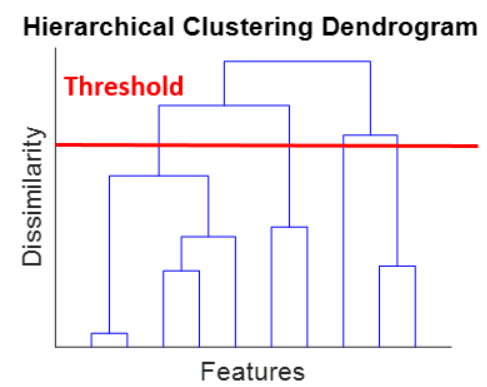
\includegraphics[scale=0.75,width=.4\linewidth]{dend.png}
	\caption{Dendrogram of Hierarchical Clustering}
	\label{fig:dendrogram}
\end{figure}

As similarity decreases or dissimilarity increases, the number of features left will decrease as several merges have occurred. If a threshold is chosen, the number of clusters left are the amount of blue lines that intersect the red threshold line. In other cases where a certain number is picked, the threshold chosen may be found based on the dendrogram but is not explicitly chosen. 

Similarly to hierarchical clustering and MNF, if the assumption is made that several features are highly correlated, it is worth investigating simply throwing out some of them. To represent this mindset one can review spectral downsampling. 

\begin{figure}[H]
	\centering
		\subfloat[Hyperspectral Cube	\label{fig:hsi}]{{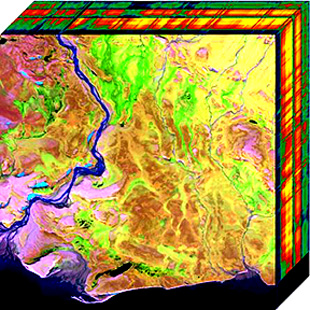
\includegraphics[width=.3\linewidth,height=4cm]{hscube}}}
\qquad
	\subfloat[Unit Porcupine\label{fig:uporc}]{{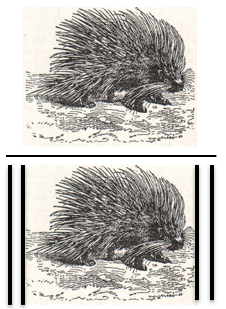
\includegraphics[width=.3\linewidth,height=4cm]{uporc}}}	
\caption{Motivation for Dimensionality Reduction}
\end{figure}
 
 Overall, each of the previously described methods attempts to deal with what can be can be easily visualized as the unit porcupine in figure \ref{fig:uporc}. In the case of our hyperspectral data (figure \ref{fig:hsi}), we have few samples compared to the dimensionality of our features (relatively speaking). As we look at some similarity or distance measure in high dimensions, data points get pushed to the quills and become infinitely far apart. To address this problem, we want to reduce the dimensionality of our dataset. This paper aims to compare the previously mentioned dimensionality reduction techniques in an unbiased way. One issue with bias is the method to quantitatively evaluate our results. To address this we will evaluate all methods using an SVM classifier on a two class problem. The rest of this paper is structured as follows: section II describes the methodology we use to select the final parameters chosen and each of the supplemental experiments we ran to select these parameters and how they were implemented, section III describes our experimental results, section IV describes our observations, lastly section V describes our conclusions. 
%%%%%%%%%%%%%%%%%%%%%%%%%%%%%%%%%%%%%%%%%%%%%%%%%%%%%%
\section{Methodology}

\subsection{Removing Bad Bands}

\begin{figure}[H]
	\centering
	\subfloat[Before bad band removal	\label{fig:PRERemove}]{{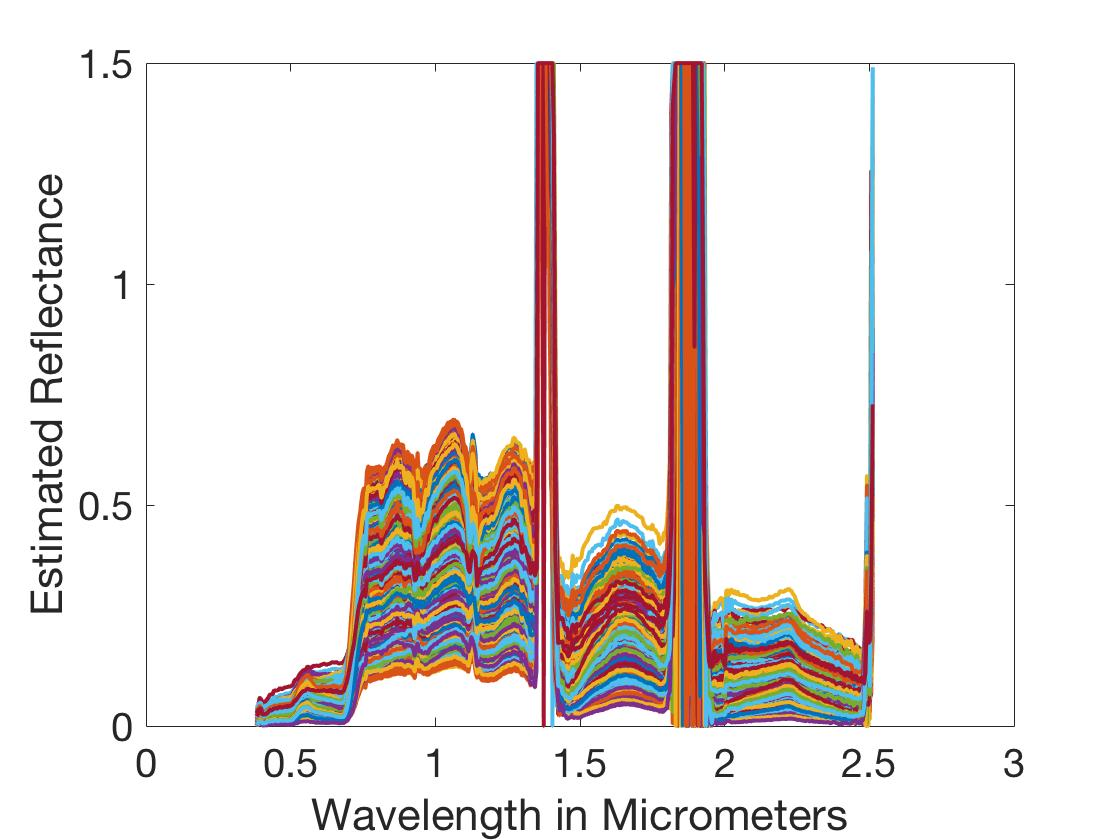
\includegraphics[height=4.25cm, width=.45\linewidth]{pre}}}
	\qquad
	\subfloat[After bad band removal \label{fig:POSTRemove}]{{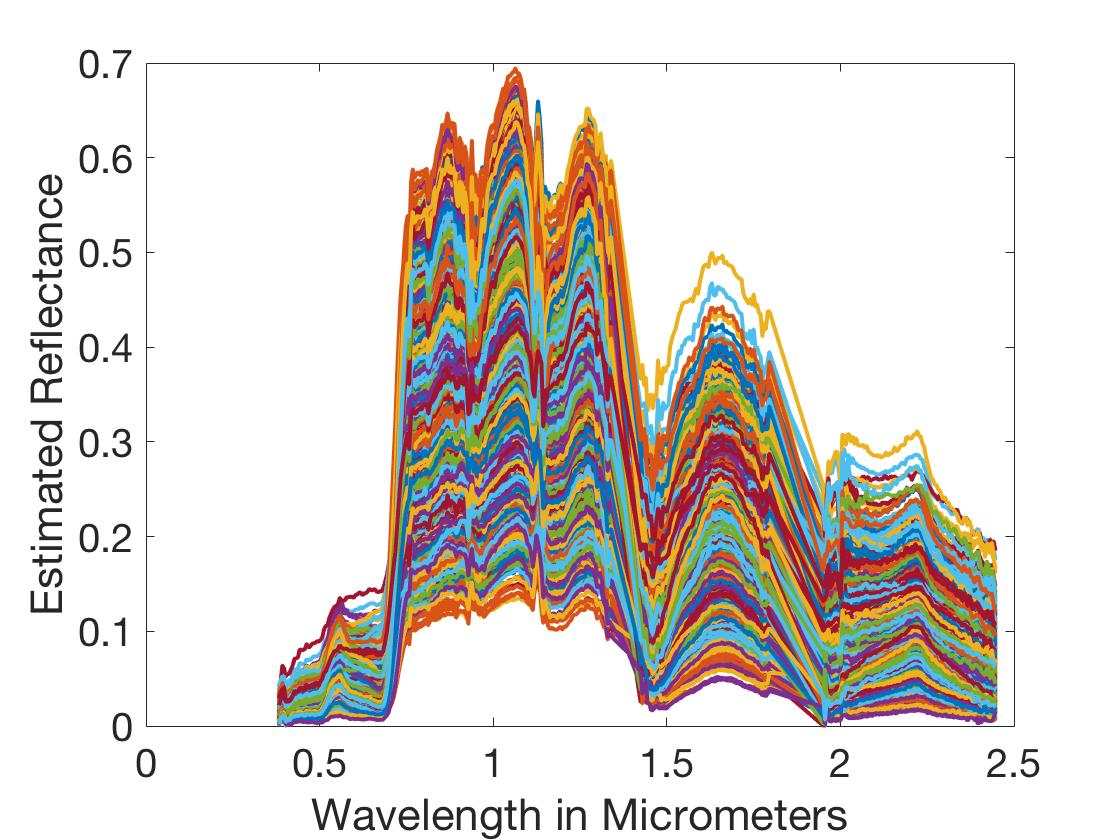
\includegraphics[height=4.25cm,width=.45\linewidth]{post}}}	
	\caption{Before and after bad band removal}
\end{figure}

\subsection{SVM Training}
Given that our objective is comparing dimensionality reduction methods and not optimizing an SVM classifier, we use the built in MATLAB SVM functions and do not modify any of the classification parameters manually. Each method is trained and tested separately and have no influence on the model parameters of any other method. 


\subsection{Principal Component Analysis}
PCA projects the data into a subspace that maximizes variance. Considering the notion of using PCA in dimensionality reduction and evaluation by classification accuracy there are two main quantitative values of importance that influence our parameter selection experiments. Mainly, how well can we classify the data using $D<B$ features or bands? More subtly, how much variance are we keeping by selecting this number of principal components? Is maximizing variance maximizing separability?

For our first experiment of comparing the number of bands, we vary the number of bands to keep $D$ from the maximum number of bands $D_{max}$ to 1 and plot the classification accuracy and variance kept. A supplemental plot of the lowest varying set of eigenvectors is also constructed. Lastly we show a plot of our data in 3 dimensions using the top 3 components and compare to the lowest 3 components that are greater than 0. 

\subsection{Maximum Noise Fraction}
Similarly to PCA, MNF is a linear projection into a subspace. However, in this case that subspace maximizes the SNR. We are interested in estimating the noise correctly. In theory, if we estimate the noise well and the classes are separable and compact, classification rate should be high. Given the parameters for MNF we choose varying amounts of noise to be added to the spectra of the classes for our MNF estimation. We also choose a varying amount of components given that we assume some bands are primarily noise. 

Given that this method relies on two main inputs (noise and number of components), we ran a single experiment that varies the variance of the noise added given 0 mean and the number of components from $D_{max}$ to 1. We aim to view the effects of each parameter individually and their possible influence on each other.

\subsection{Hierarchical Dimensionality Reduction}
Unlike the previous methods, HDR is not a linear projection. HDR merges similar bands and therefore we must only consider modifying the number of bands desired and how we compute similarity. In the code we were given, our HDR is performed by merging the two most similar bands by their Jensen-Shannon Divergence (JSD) \cite{JSD}. Given that the author of this paper has yet to publish his methods on comparing high-dimensional distributions, we decided to modify HDR with JSD by using a parzen window estimator \cite{parzen}.

For this method we will run experiments with varying numbers of bands and compare the performance of the JSD with and without parzen window estimation.

\subsection{Spectral Downsampling}
Given that this method is simply throwing out bands and averaging them we conduct an experiment with varying number of bands for averaging a group of bands and compute the classification accuracy.

\section{Results}
We first looked at each method over the training data.

\begin{figure}[H]
	\centering
	\subfloat[Full Image Training	\label{fig:FIT}]{{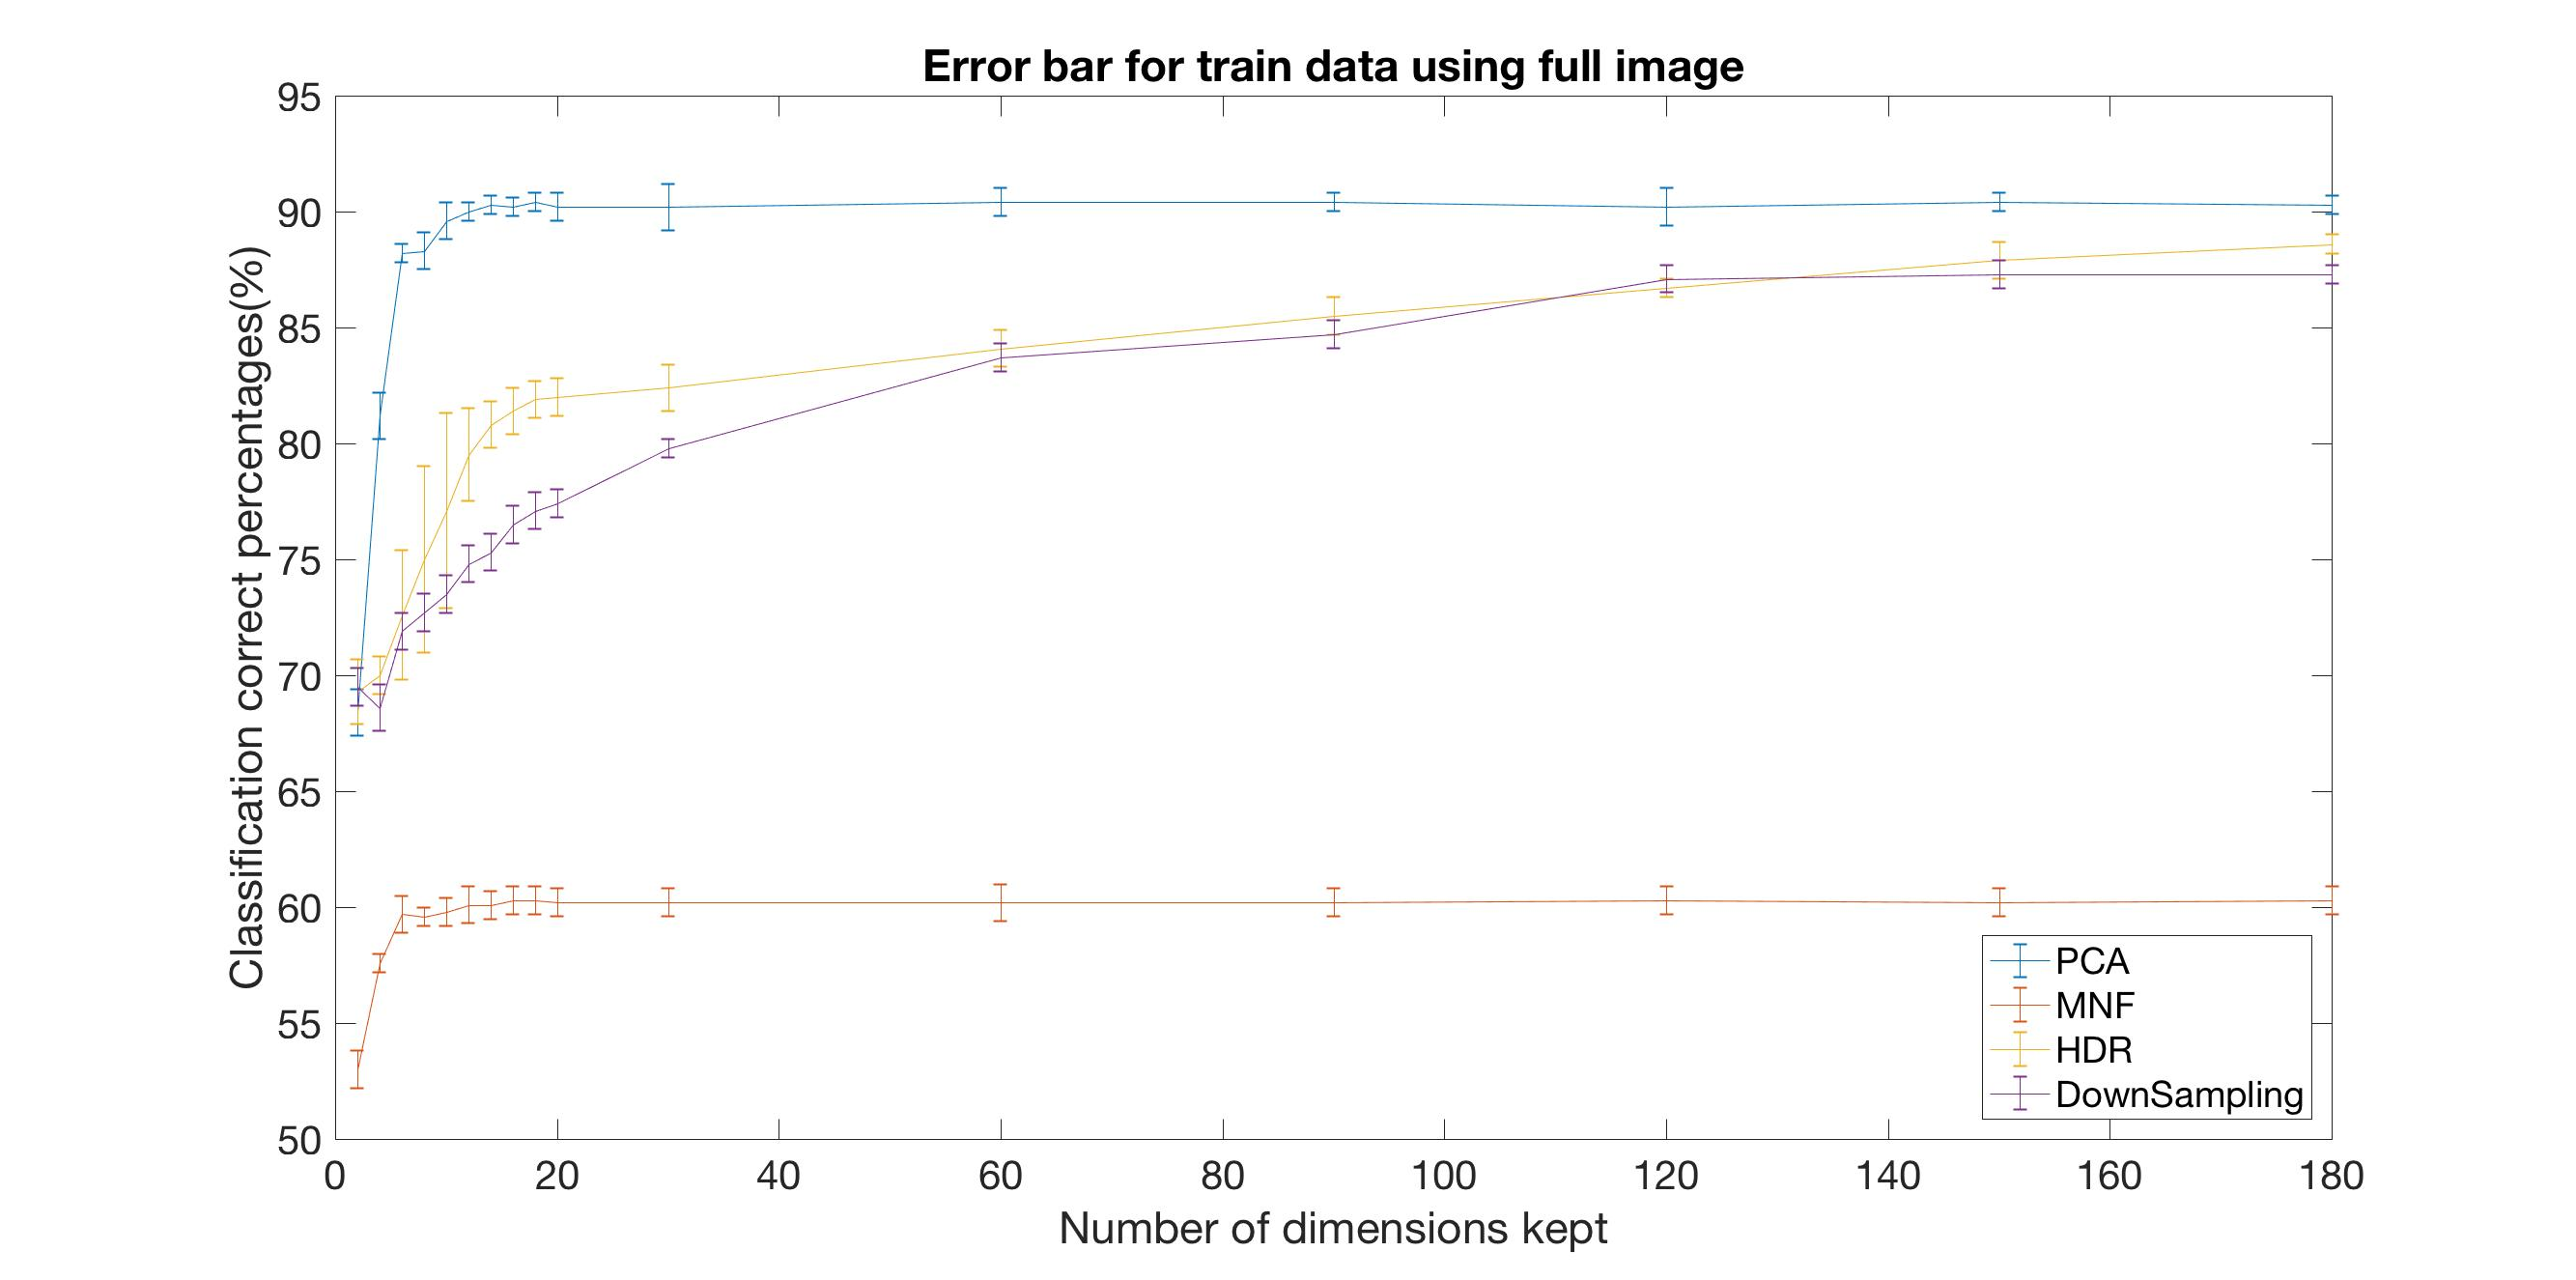
\includegraphics[width=.45\linewidth]{fullTrain}}}
	\qquad
	\subfloat[Class Specific Training\label{fig:CST}]{{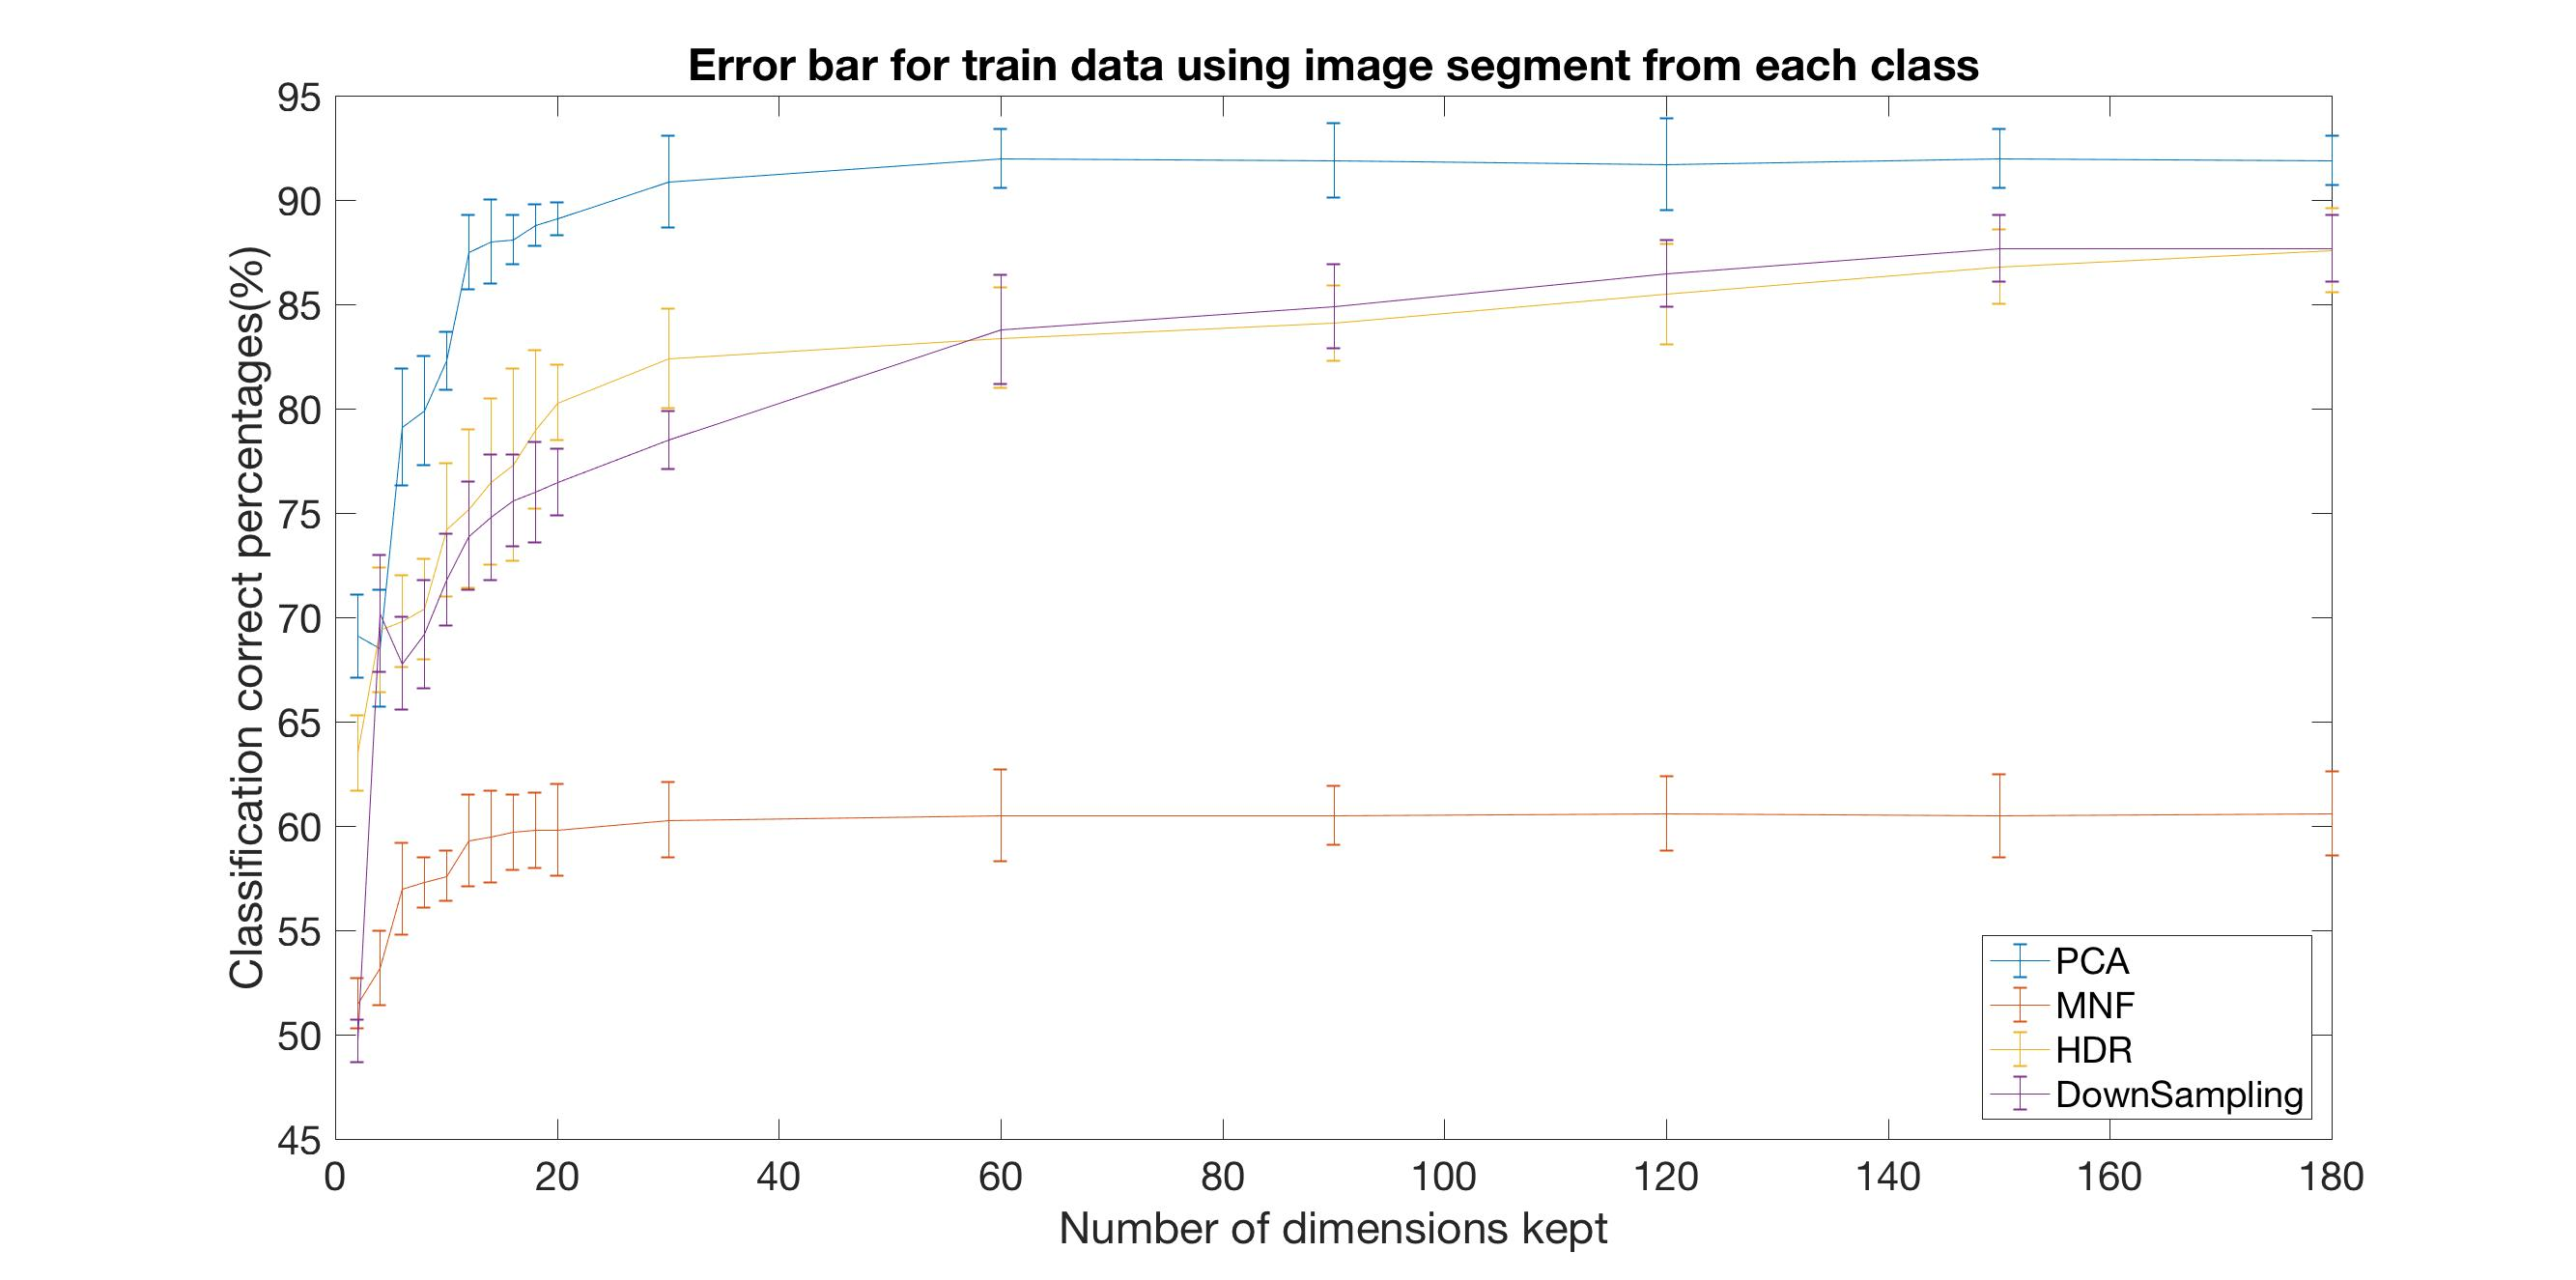
\includegraphics[width=.45\linewidth]{classTrain}}}	
	\caption{10 fold cross-validation means and 2 standard deviation error bars}
\end{figure}



\subsection{Principal Component Analysis}

Our first PCA experiment compares PCA given a specific number of bands. In order to understand how much variance we are keeping we look at the variance from samples of the full image in relation to the number of kept principal components.

\begin{figure}[H]
	\centering
	\subfloat[PCA Training	\label{fig:PCAEXPCval}]{{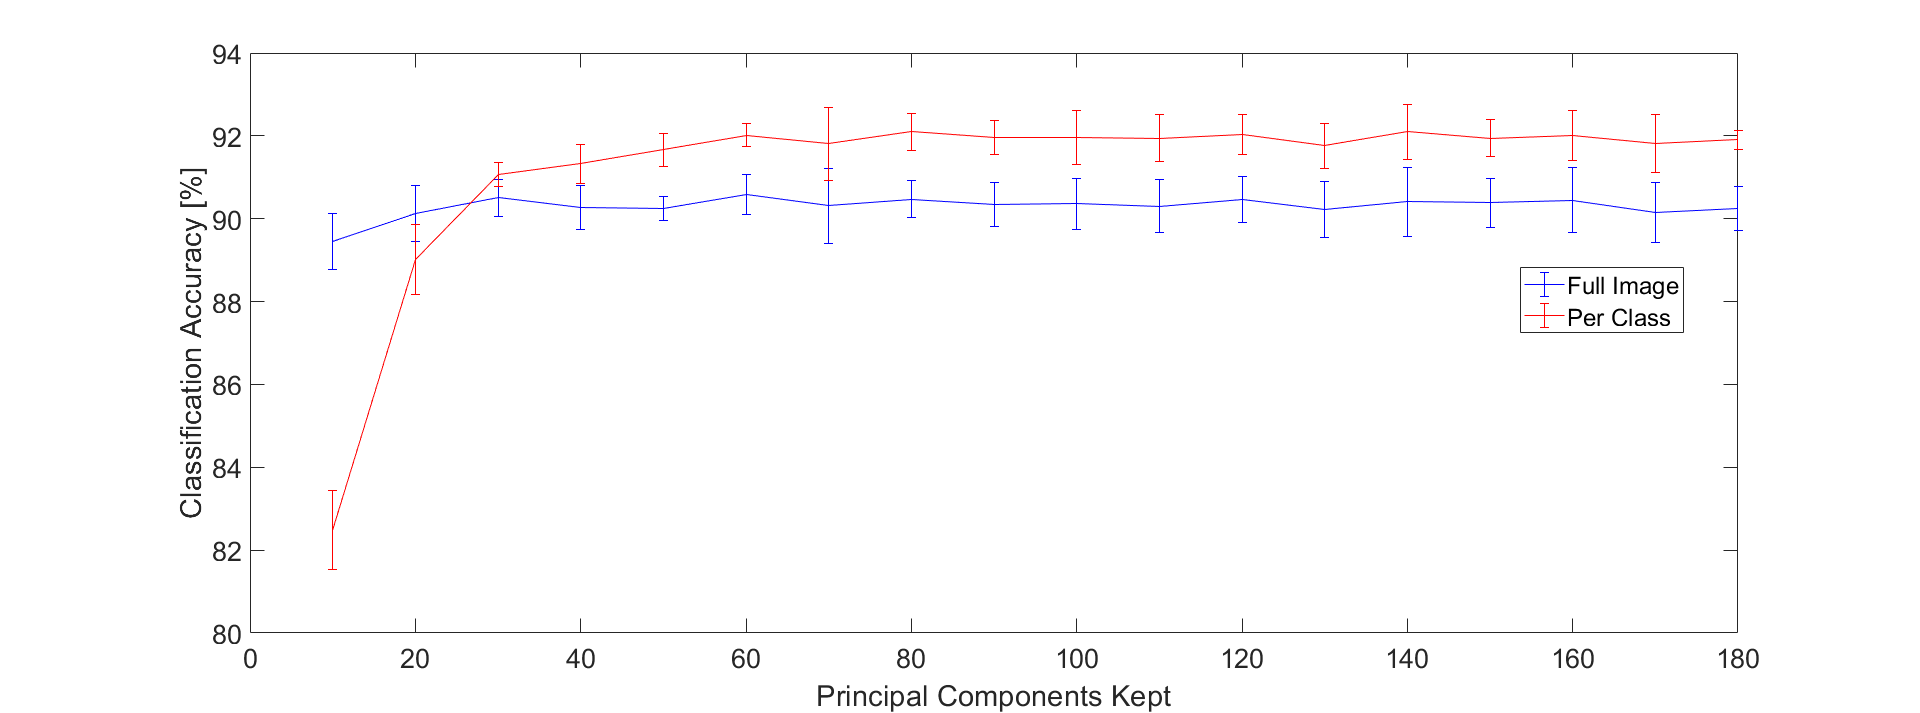
\includegraphics[width=.45\linewidth]{classaccpca}}}
	\qquad
	\subfloat[Variance over 1 run \label{fig:PCAEXPVar}]{{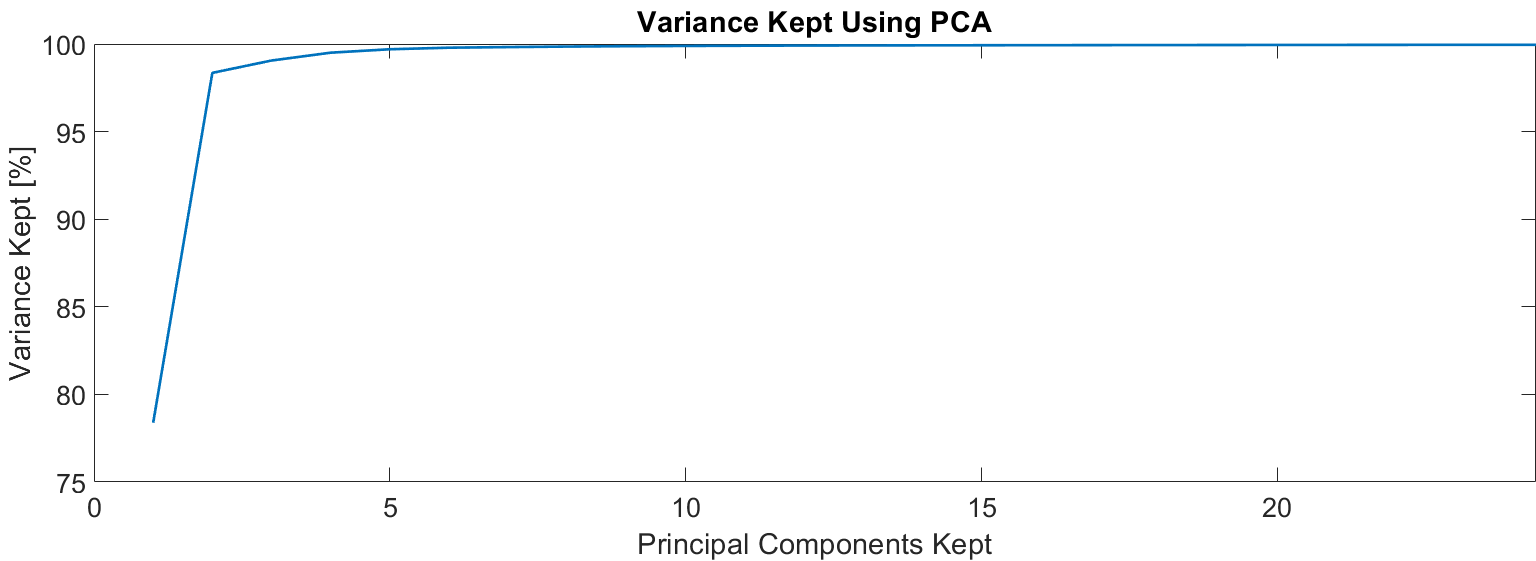
\includegraphics[width=.45\linewidth]{varkept}}}	
	\caption{10 fold cross-validation means and 2 standard deviation error bars for training and $\%$ variance kept for one run}
\end{figure}

We also look at the projection of the data in 3 dimensions.
\begin{figure}[H]
	\centering
	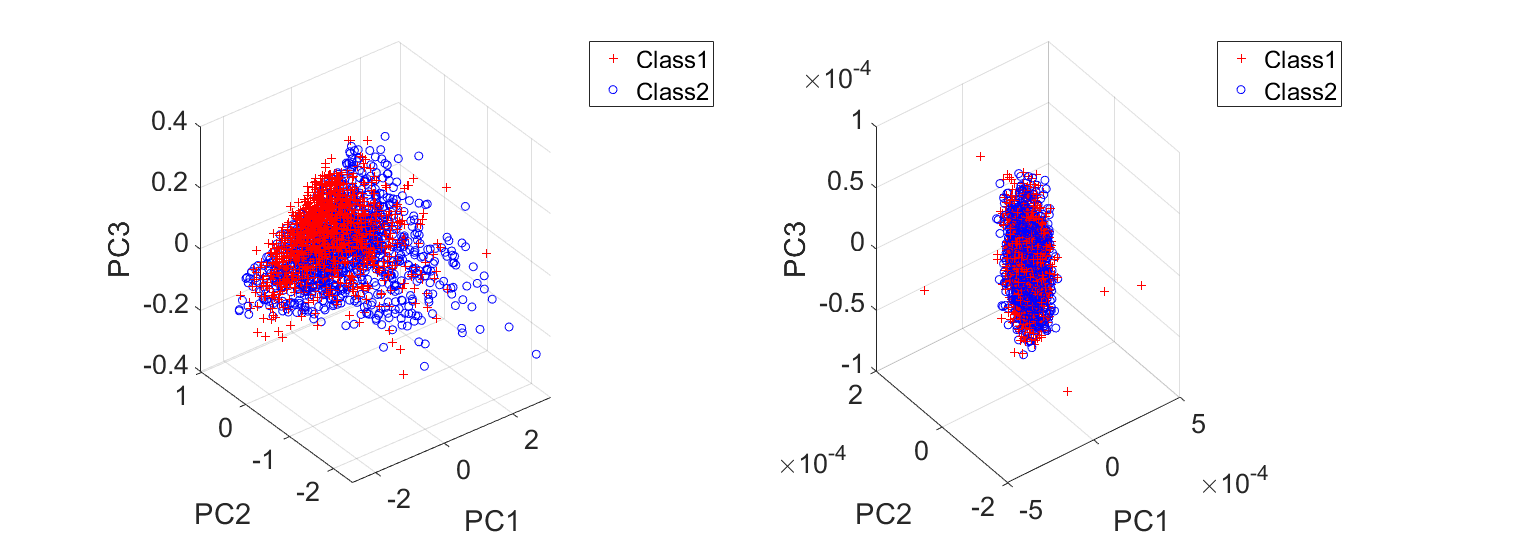
\includegraphics[height=4cm,width=\linewidth]{top3bot3}
	\caption{L:R Top 3 and bottom 3 PCA components}
	\label{PCAEXP3D}
\end{figure}

\subsection{Maximum Noise Fraction}
%%%%%%% include stuff here
Similar to PCA we looked at the first and last 3 components of MNF to view possible separation.

\begin{figure}[H]
	\centering
	\subfloat[Top 3 MNF Components	\label{fig:MNFTOP3}]{{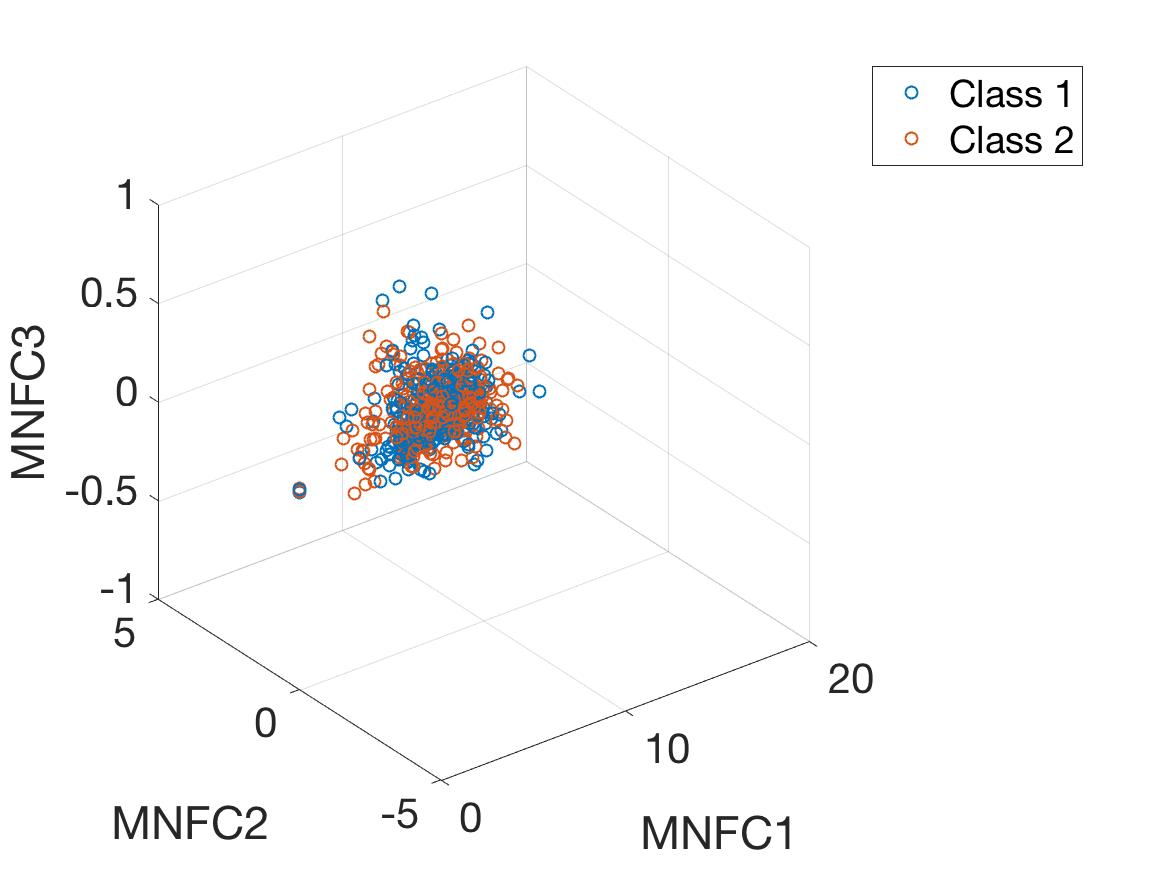
\includegraphics[height=4cm,width=.45\linewidth]{first3MNFtrain}}}
	\qquad
	\subfloat[Last 3 MNF Components \label{fig:MNFBOT3}]{{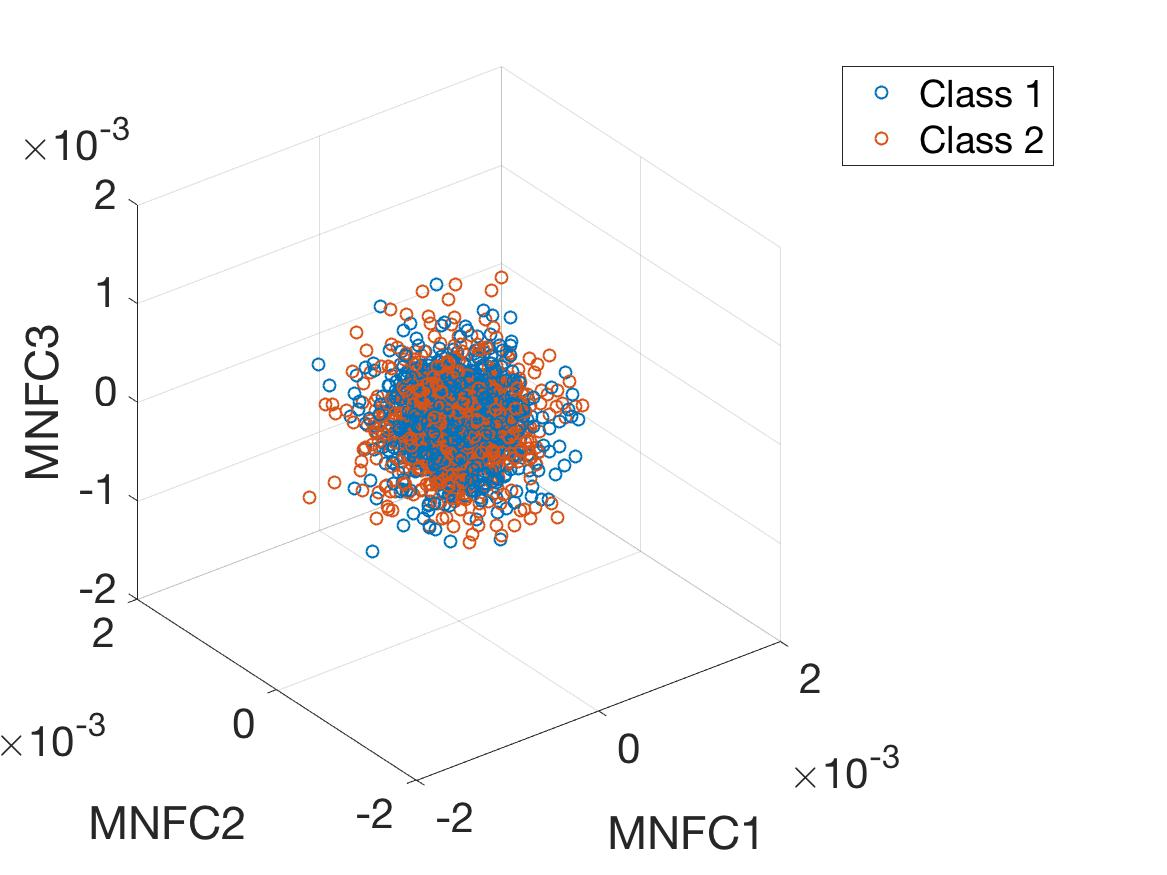
\includegraphics[height=4cm,width=.45\linewidth]{last3MNFtrain}}}	
	\caption{Top 3 and bottom 3 MNF components}
\end{figure}

If we add noise with different covariances or different diagonal loading numbers, the results are shown below:
\begin{figure}[H]
	\centering
	\subfloat[Different performances with different covariance matrix of the noise added \label{fig:MNFTOP3}]{{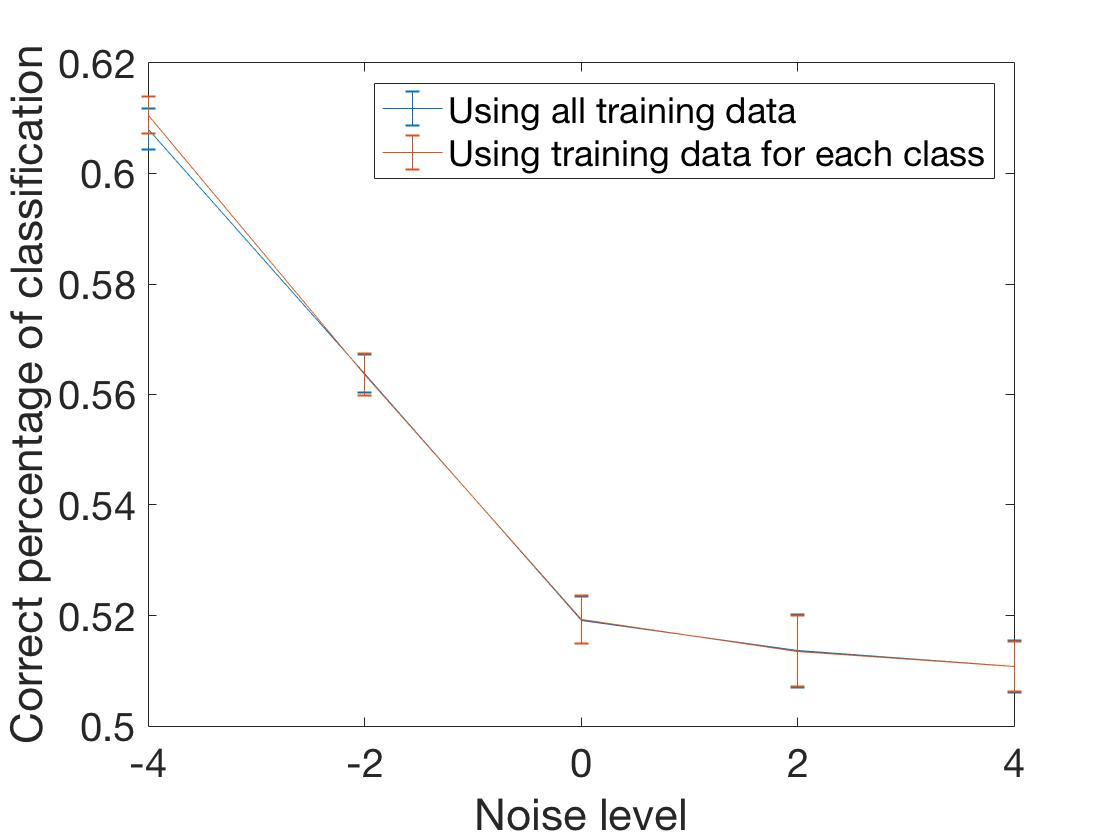
\includegraphics[width=.45\linewidth]{MNFcovariancelevel}}}
	\qquad
	\subfloat[Different performances with different diagonal loading factor \label{fig:MNFBOT3}]{{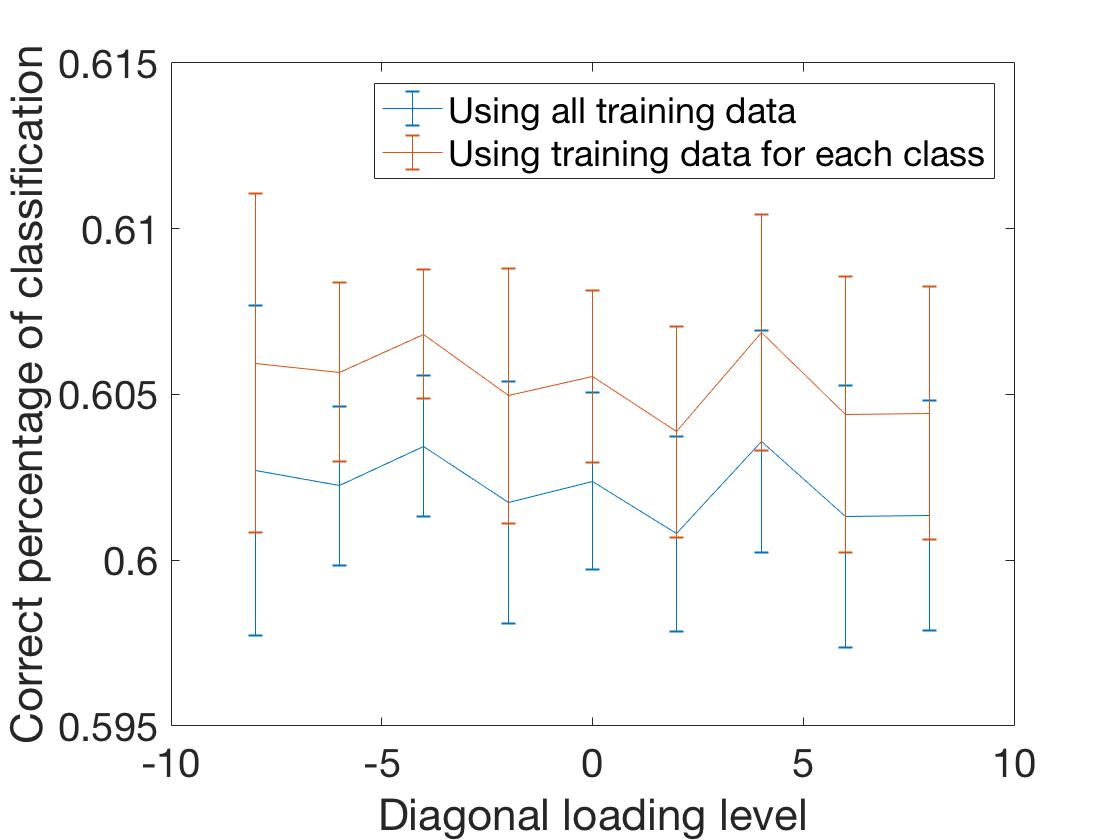
\includegraphics[width=.45\linewidth]{MNFdiaglevel}}}	
	\caption{The effect of different covariance matrices or diagonal loading factors. }
\end{figure}


\subsection{Hierarchical Clustering}
For Hierarchical Clustering we ran experiments with and without a parzen window estimator with window size 4.
\begin{figure}[H]
	\centering
	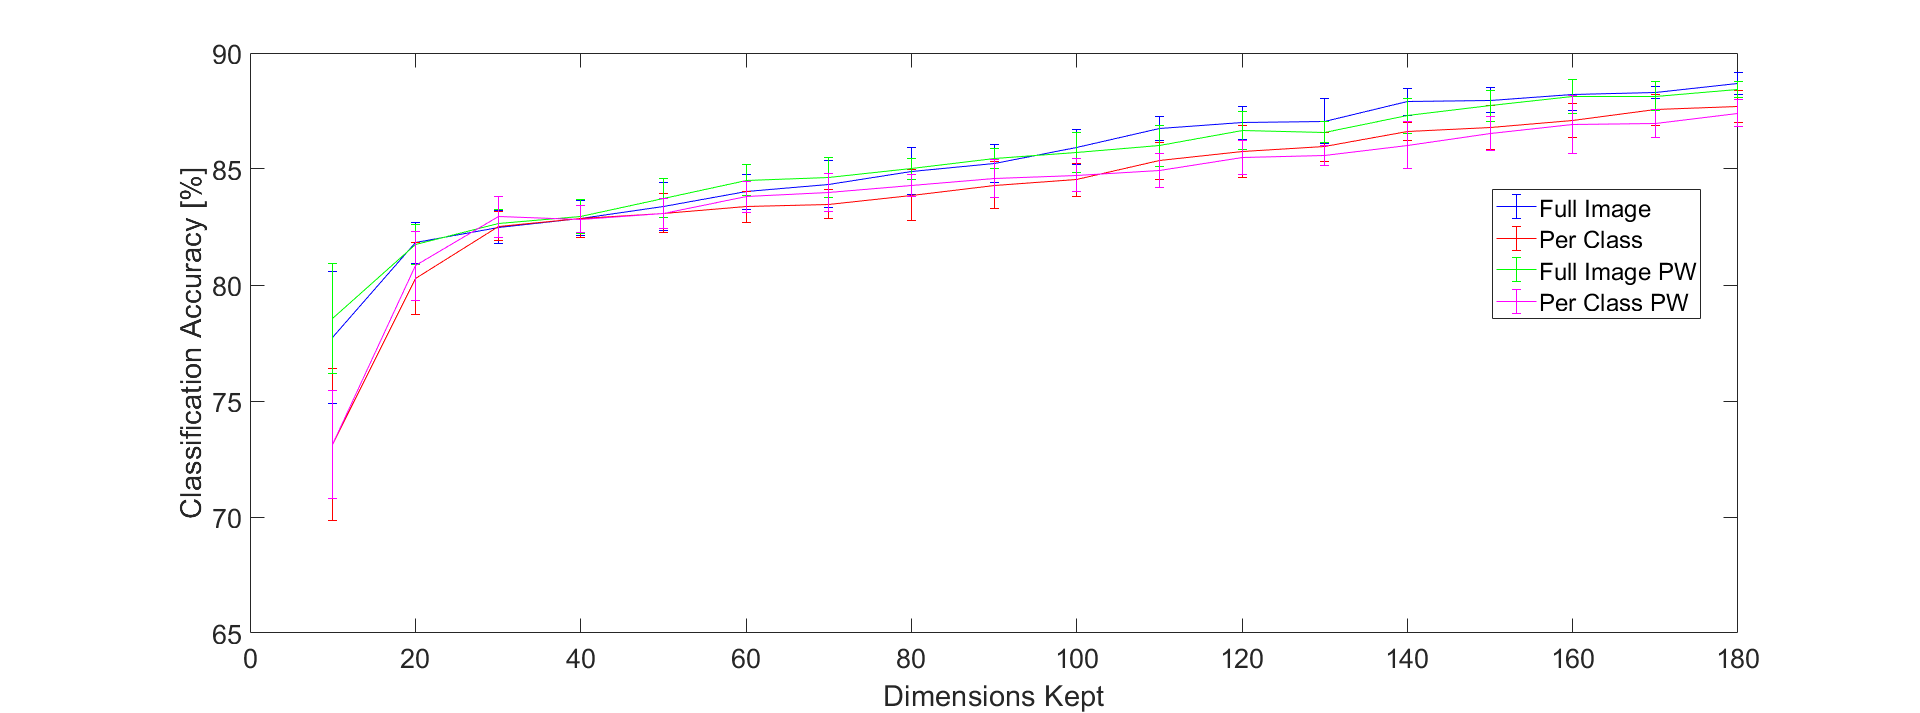
\includegraphics[scale=0.2]{hdrclassacc}
	\caption{10 fold cross-validation with means and 2 standard deviation in error bars}
	\label{HDREXP}
\end{figure}

We also wanted to look at which bands have the smallest KL-divergence to ensure that the method is picking similar bands.

\begin{figure}[H]
	\centering
	\subfloat[Similarity between bands using parzen windowed smoothed pdf and KL-Divergence	\label{fig:HDRSimMat}]{{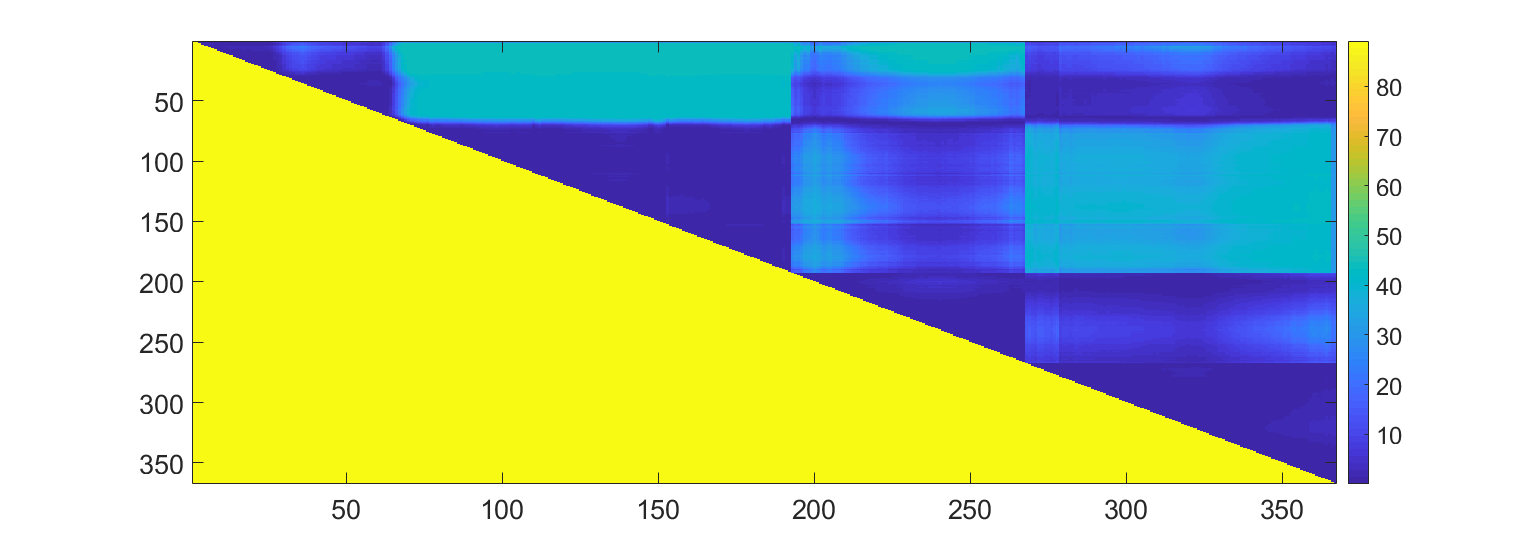
\includegraphics[height=3.5cm,width=.45\linewidth]{hdrsimmat}}}
	\qquad
	\subfloat[Most similar bands using parzen windowed smoothed pdf and KL-Divergence \label{fig:HDRMostSim}]{{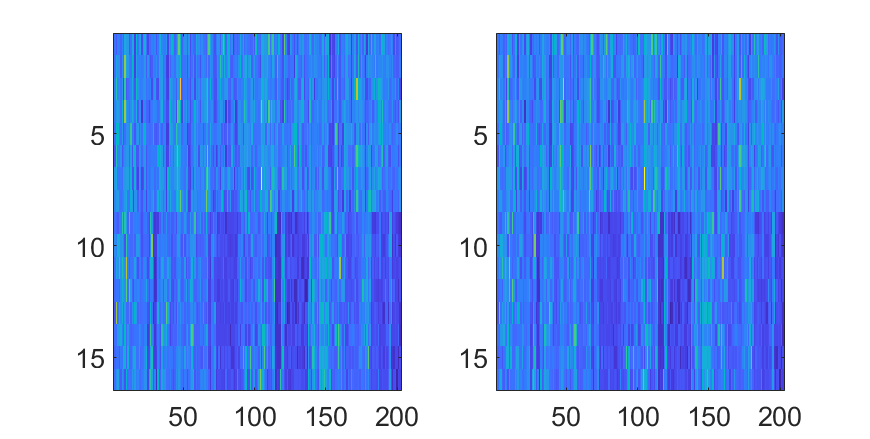
\includegraphics[height=3.5cm,width=.45\linewidth]{hdrwv21wv22}}}	
	\caption{Verifying parzen window and KL-divergence}
\end{figure}

Classification results for the full image and per class are shown in tables I and II and tables III and IV respectively.
\begin{table*}[!htb]
	\begin{minipage}{.4\linewidth}
		\centering
		\begin{tabular}{lcccc}
			\hline
			No. experiment & PCA & MNF & HDR & Down sampling\\
			\hline
			1 &  90 &  60 & 81 & 78 \\
			2 &  90 &  60 & 83 & 77 \\
			3 &  90 &  60 & 82 & 77 \\
			4 &  90 &  60 & 82 & 77 \\
			5 &  90 &  60 & 82 & 78 \\
			6 &  90 &  60 & 82 & 77 \\
			7 &  90 &  60 & 81 & 77 \\
			8 &  90 &  60 & 82 & 78 \\
			9 &  90 &  60 & 82 & 78 \\
			10 &  90 &  93 & 86 & 87 \\
			\hline
			mean & 90.2 & 60.2 & 82.0 & 77.4 \\
			std.dev & 0.3 & 0.3 & 0.4 & 0.3\\
			\hline
		\end{tabular}
		\caption{Table of training correct percentages when using whole data set to reduce dimensionality}
	\end{minipage}
	\qquad
	\qquad
	\qquad
	\qquad
	\begin{minipage}{.4\linewidth}
		\begin{tabular}{lcccc}
			\hline
			No. experiment & PCA & MNF & HDR & Down sampling\\
			\hline
			1 &  91 &  61 & 82 & 76 \\
			2 &  90 &  60 & 82 & 77 \\
			3 &  90 &  60 & 81 & 77 \\
			4 &  90 &  59 & 82 & 77 \\
			5 &  90 &  61 & 81 & 77 \\
			6 &  89 &  60 & 81 & 77 \\
			7 &  91 &  59 & 83 & 78 \\
			8 &  90 &  61 & 83 & 76 \\
			9 &  90 &  58 & 81 & 77 \\
			10 &  90 & 61 & 82 & 77 \\
			\hline
			mean & 90.1 & 60.1 & 81.7 & 77.0 \\
			std.dev & 0.1 & 1.1 & 0.6 & 0.7\\
			\hline
		\end{tabular}
		\caption{Table of test correct percentages when using whole data set to reduce dimensionality}
	\end{minipage}
	\label{tab: t1}
\end{table*}
\begin{table*}[!htb]
	\begin{minipage}{.4\linewidth}
		\centering
		\begin{tabular}{lcccc}
			\hline
			No. experiment & PCA & MNF & HDR & Down sampling\\
			\hline
			1 &  89 &  59 & 80 & 77 \\
			2 &  89 &  60 & 81 & 76 \\
			3 &  89 &  60 & 81 & 76 \\
			4 &  89 &  60 & 81 & 77 \\
			5 &  89 &  60 & 80 & 77 \\
			6 &  90 &  60 & 81 & 76 \\
			7 &  89 &  60 & 78 & 76 \\
			8 &  89 &  60 & 79 & 77 \\
			9 &  89 &  60 & 80 & 77 \\
			10 &  89 &  59 & 81 & 77 \\
			\hline
			mean & 89.1 & 59.8 & 80.3 & 76.5 \\
			std.dev & 0.3 & 0.3 & 1.2 & 0.4\\
			\hline
		\end{tabular}
		\caption{Table of training correct percentages when reduce dimensionality for each class}
	\end{minipage}
	\qquad
	\qquad
	\qquad
	\qquad
	\begin{minipage}{.4\linewidth}
		\centering
		\begin{tabular}{lcccc}
			\hline
			No. experiment & PCA & MNF & HDR & Down sampling\\
			\hline
			1 &  89 &  61 & 79 & 76 \\
			2 &  89 &  60 & 82 & 76 \\
			3 &  89 &  60 & 80 & 77 \\
			4 &  89 &  59 & 81 & 76 \\
			5 &  89 &  60 & 79 & 76 \\
			6 &  89 &  60 & 81 & 76 \\
			7 &  89 &  59 & 79 & 78 \\
			8 &  90 &  60 & 79 & 75 \\
			9 &  89 &  57 & 79 & 76 \\
			10 &  88 & 61 & 81 & 76 \\
			\hline
			mean & 89.0 & 59.6 & 80.0 & 76.3 \\
			std.dev & 0.4 & 1.1 & 0.9 & 0.8\\
			\hline
		\end{tabular}
		\caption{Table of test correct percentages when reduce dimensionality for each class}
	\end{minipage}
	\label{tab: t2}
\end{table*}

\subsection{Pavia MNF}

For the Pavia data set, two versions of original data set are presented: the Pavia and the squeezed Pavia. The visualization of the mean over all bands for both of the fake images are shown below:
\begin{figure}[H]
	\centering
	\subfloat{{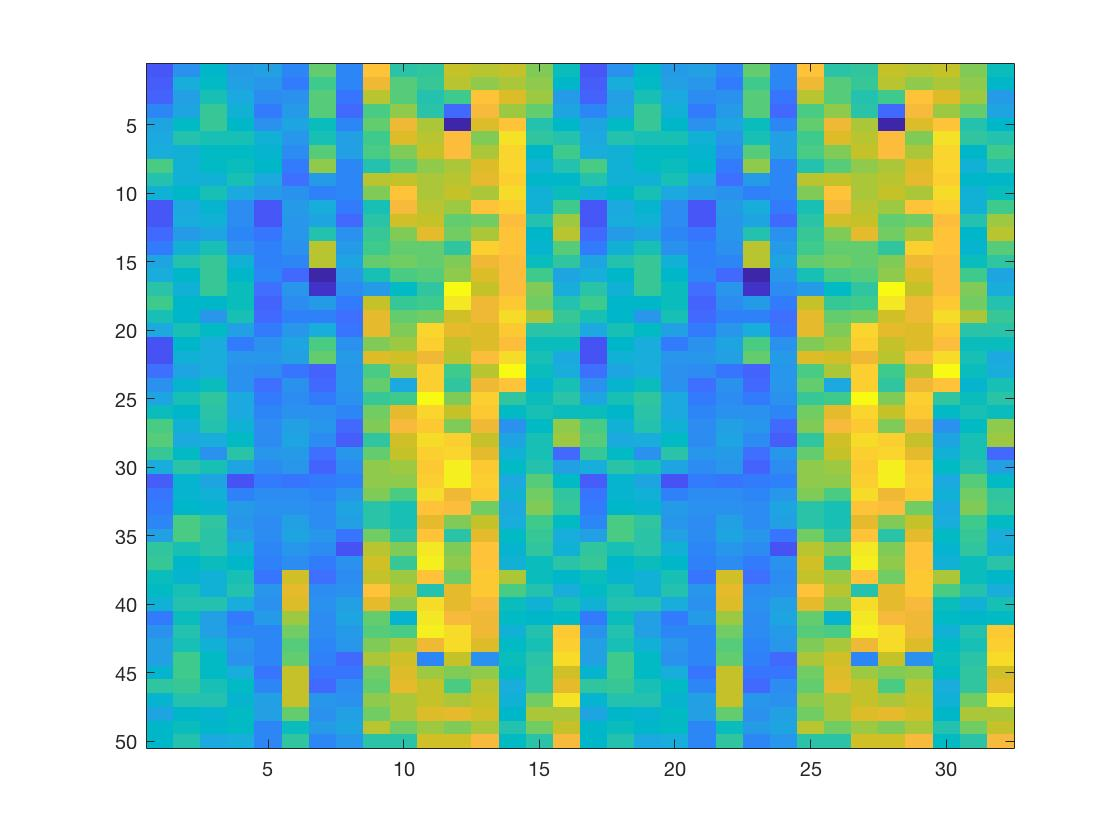
\includegraphics[width=.40\linewidth]{pavia1.jpg}}}
	\qquad
	\subfloat{{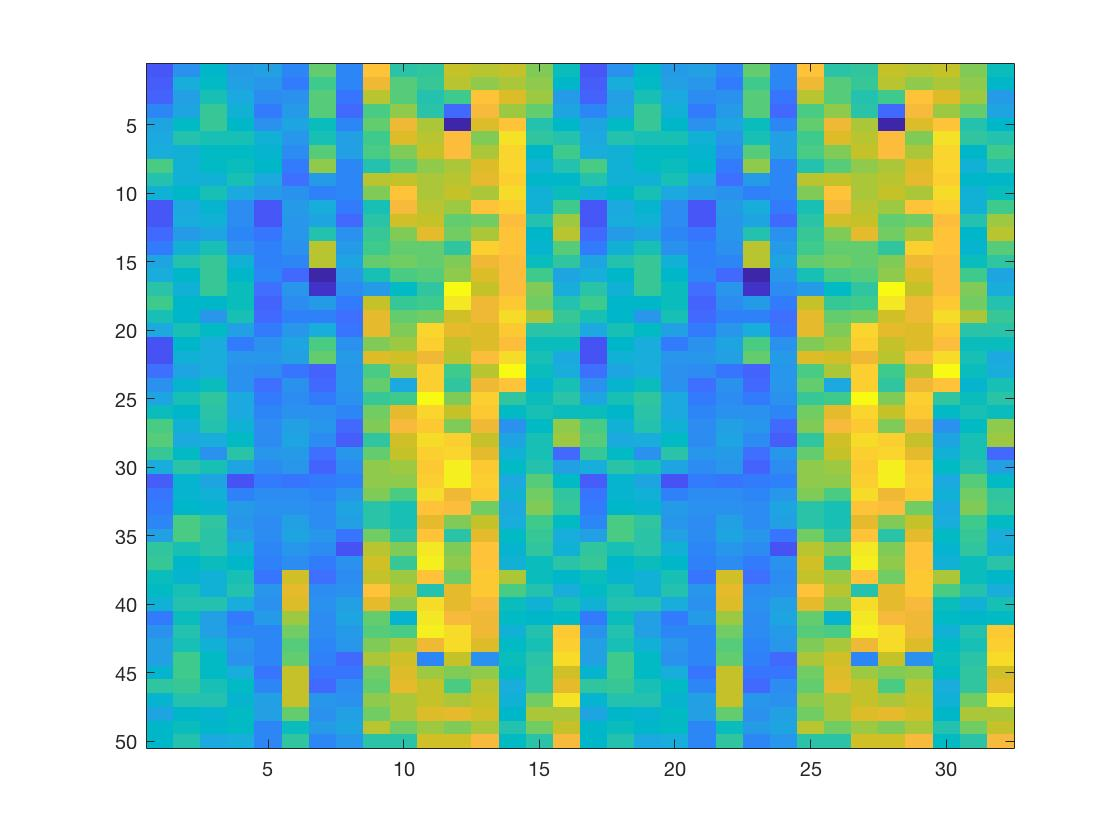
\includegraphics[width=.40\linewidth]{paviaSq1.jpg}}}	
	\caption{Visualization of mean value of the original data set over all bands. Left: fake Pavia image. Right: squeezed fake Pavia image.}
\end{figure}

\begin{figure}[H]
	\centering
	\subfloat{{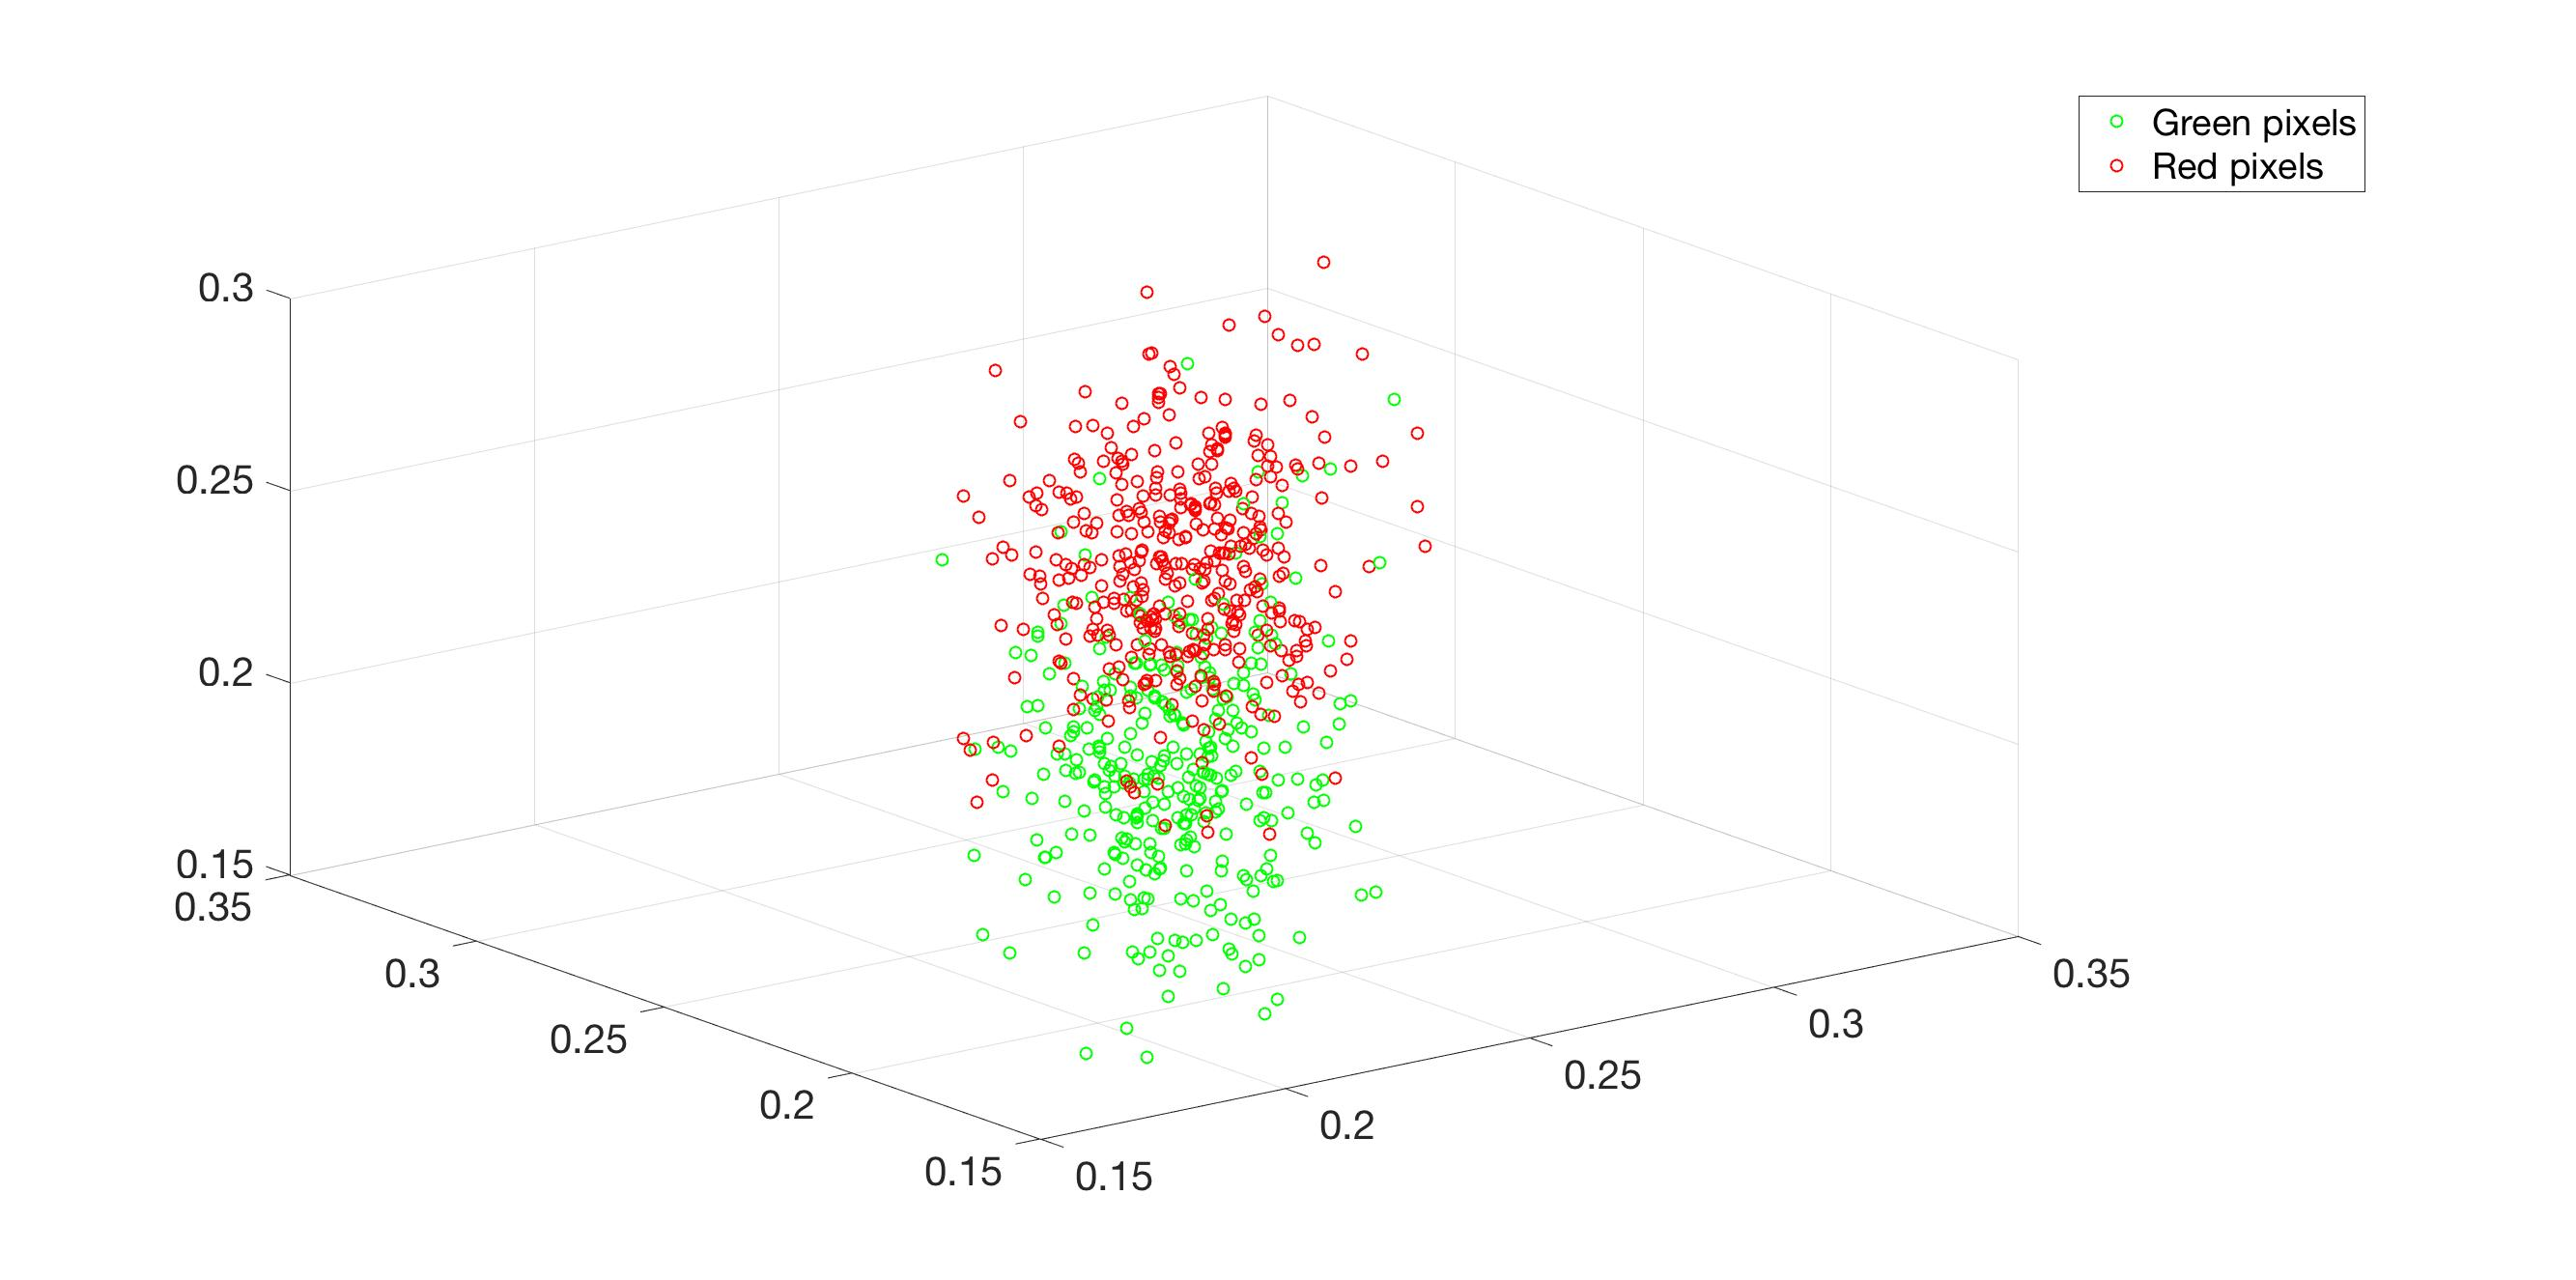
\includegraphics[width=.40\linewidth]{scatterPavia.jpg}}}
	\qquad
	\subfloat{{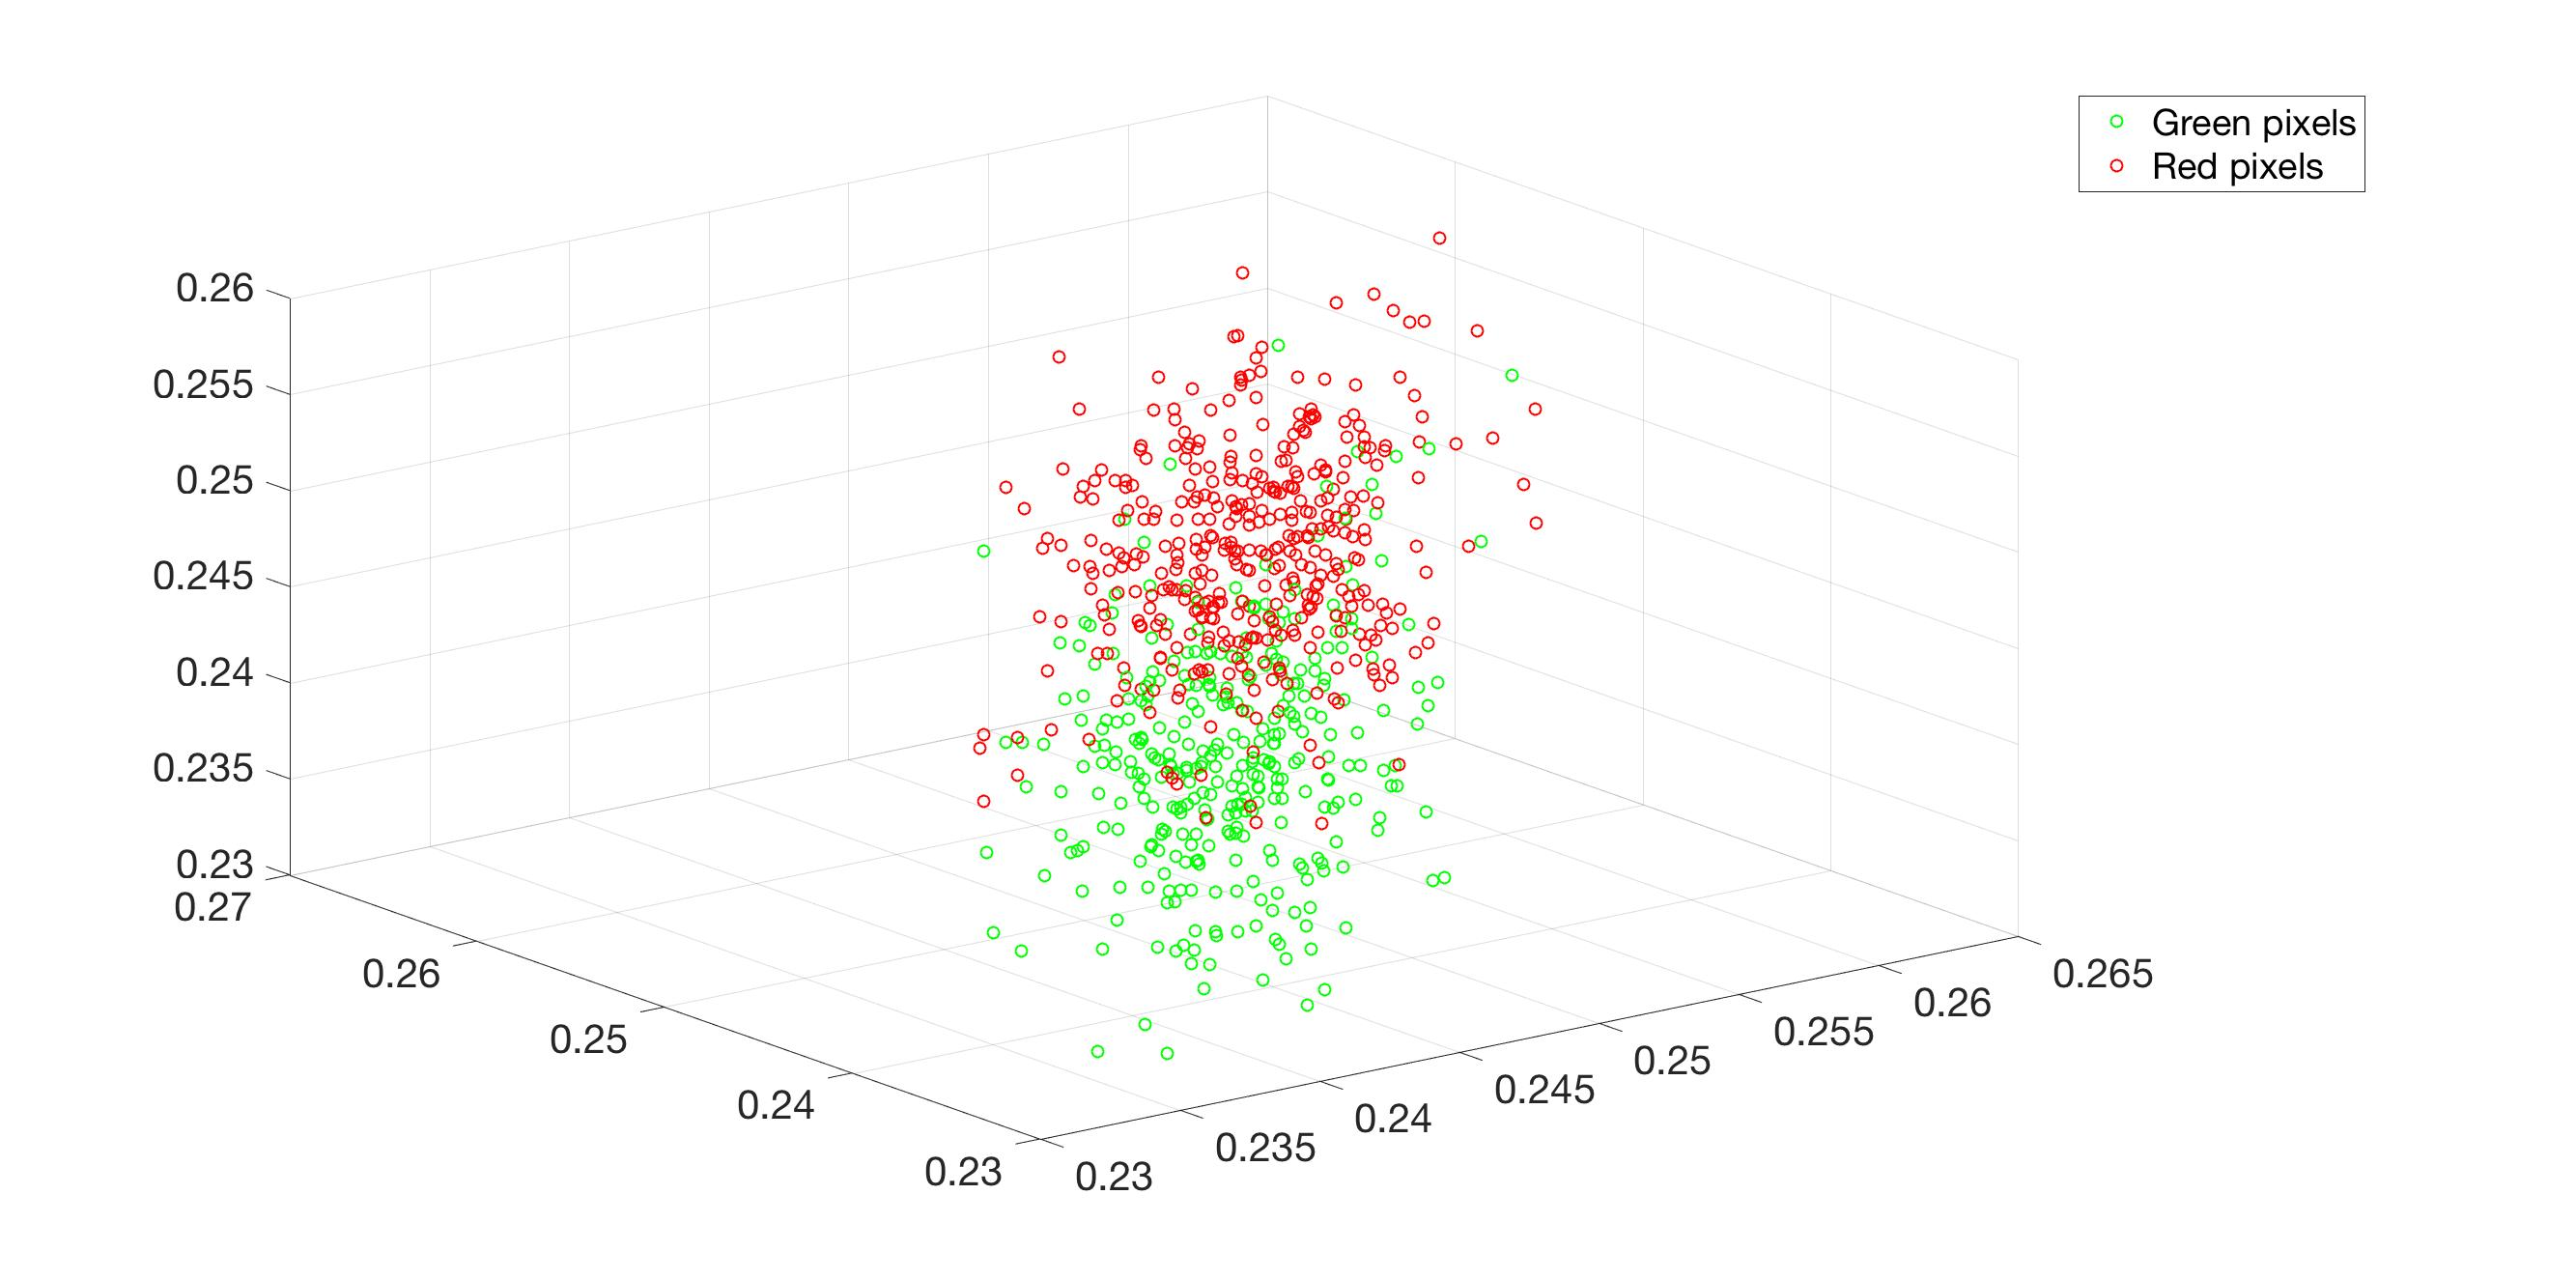
\includegraphics[width=.40\linewidth]{scatterPaviaSqueezed.jpg}}}	
	\caption{Scatter plots of the original data set before dimensionality reduction. Left: fake Pavia image. Right: squeezed fake Pavia image.}
\end{figure}

The noise levels are changed to be $10^{-4}, 10^{-2}, 1, 10^{2}, 10^{4}$, the  mean over all bands with noise added for the fake Pavia image are shown below in figure \ref{Paviamean}; the corresponding mean over all bands with dimensionality reduced results are shown in figure \ref{Paviamnfmean}; and the corresponding scatter plot of first 3 components after dimensionality using MNF are shown in figure \ref{Paviamnfscatter}.
\begin{figure}[H]
	\centering
	\subfloat{{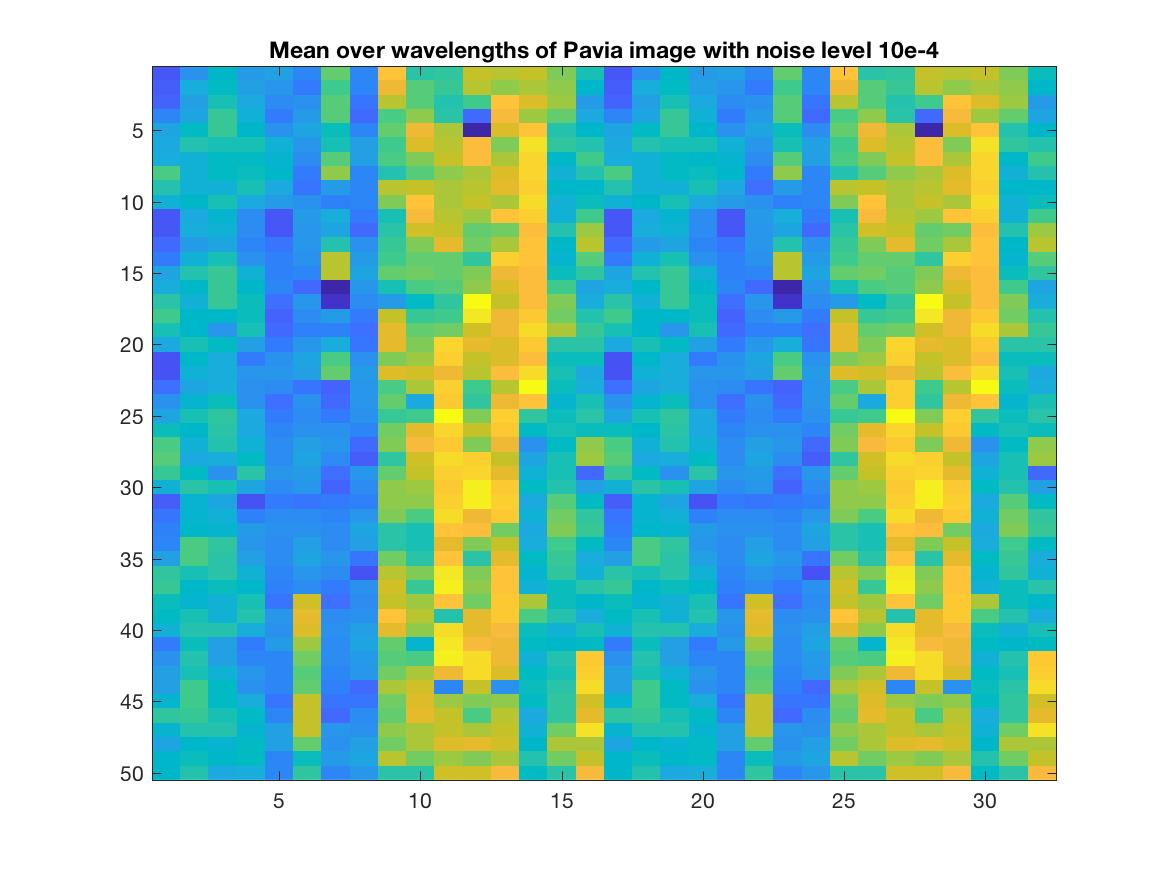
\includegraphics[width=.18\linewidth]{mean-4.jpg}}}
	\subfloat{{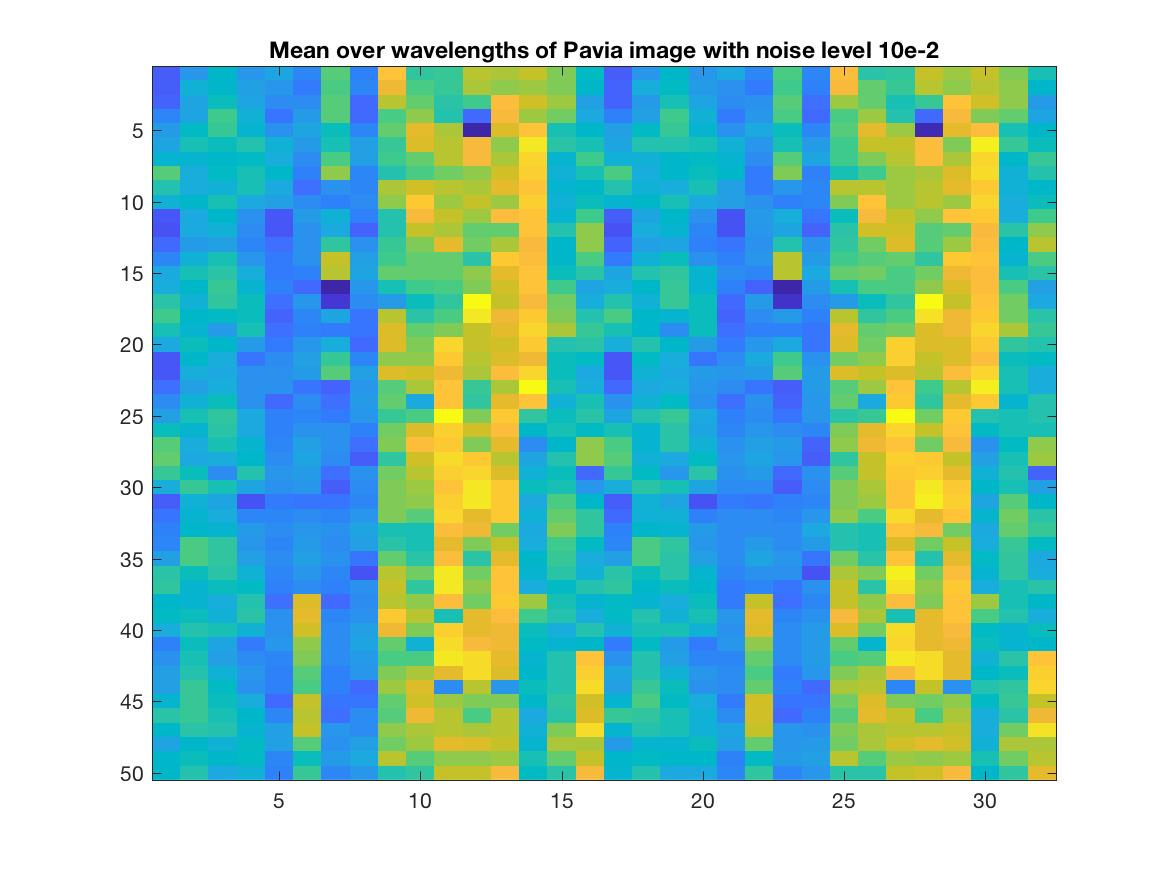
\includegraphics[width=.18\linewidth]{mean-2.jpg}}}	
	\subfloat{{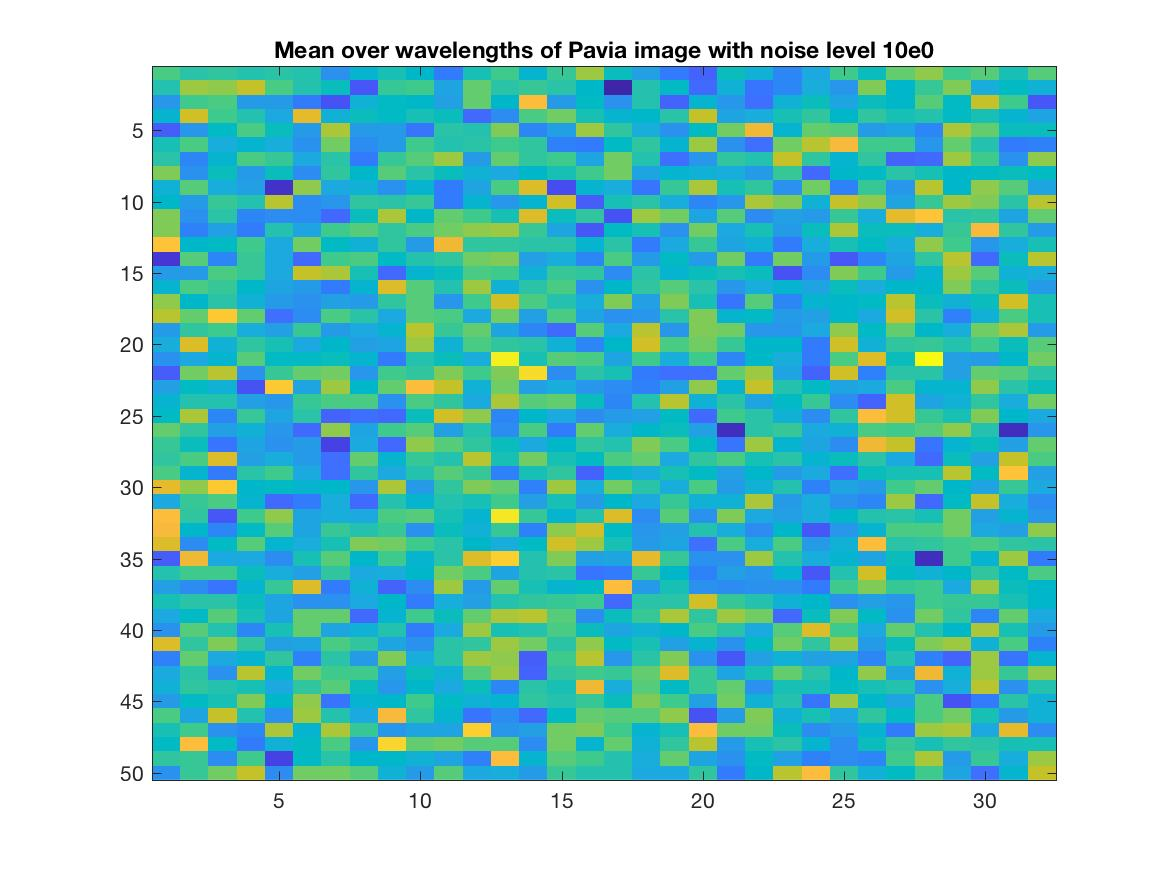
\includegraphics[width=.18\linewidth]{mean0.jpg}}}	
	\subfloat{{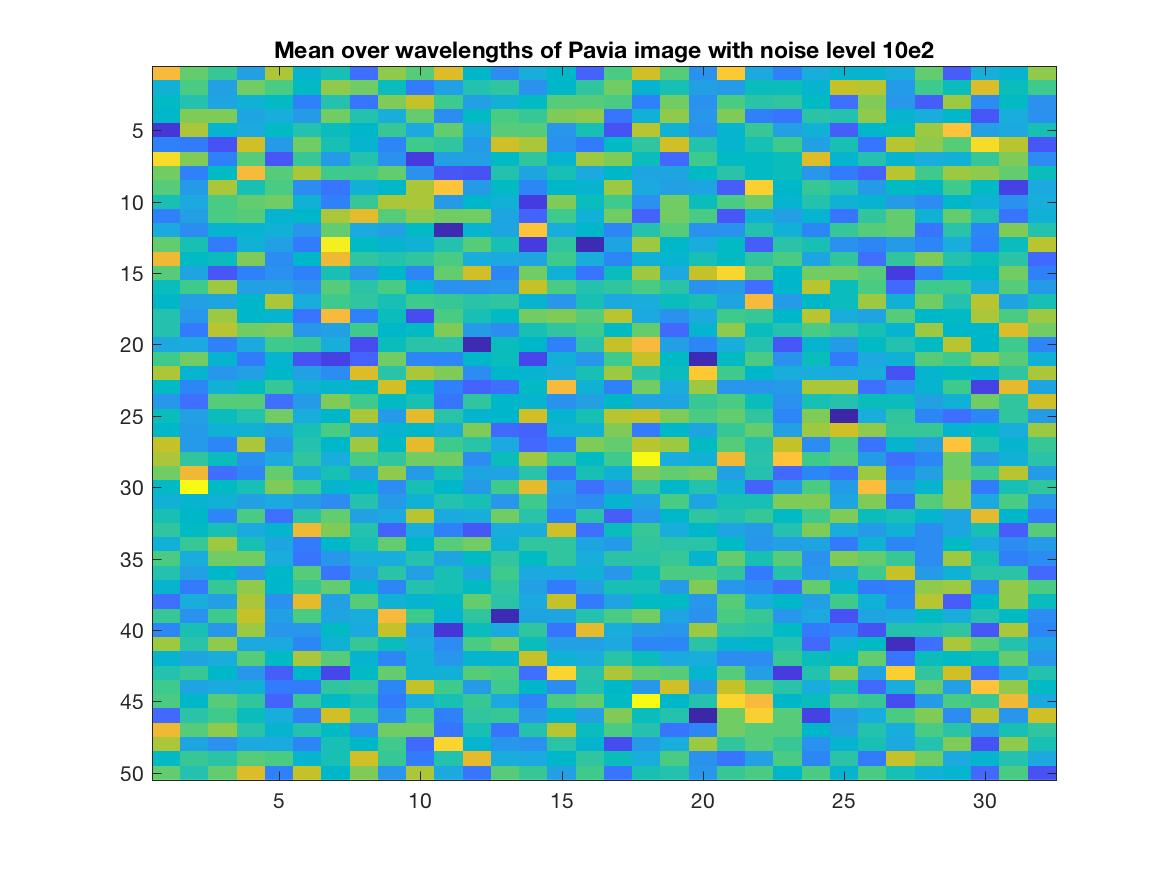
\includegraphics[width=.18\linewidth]{mean2.jpg}}}	
	\subfloat{{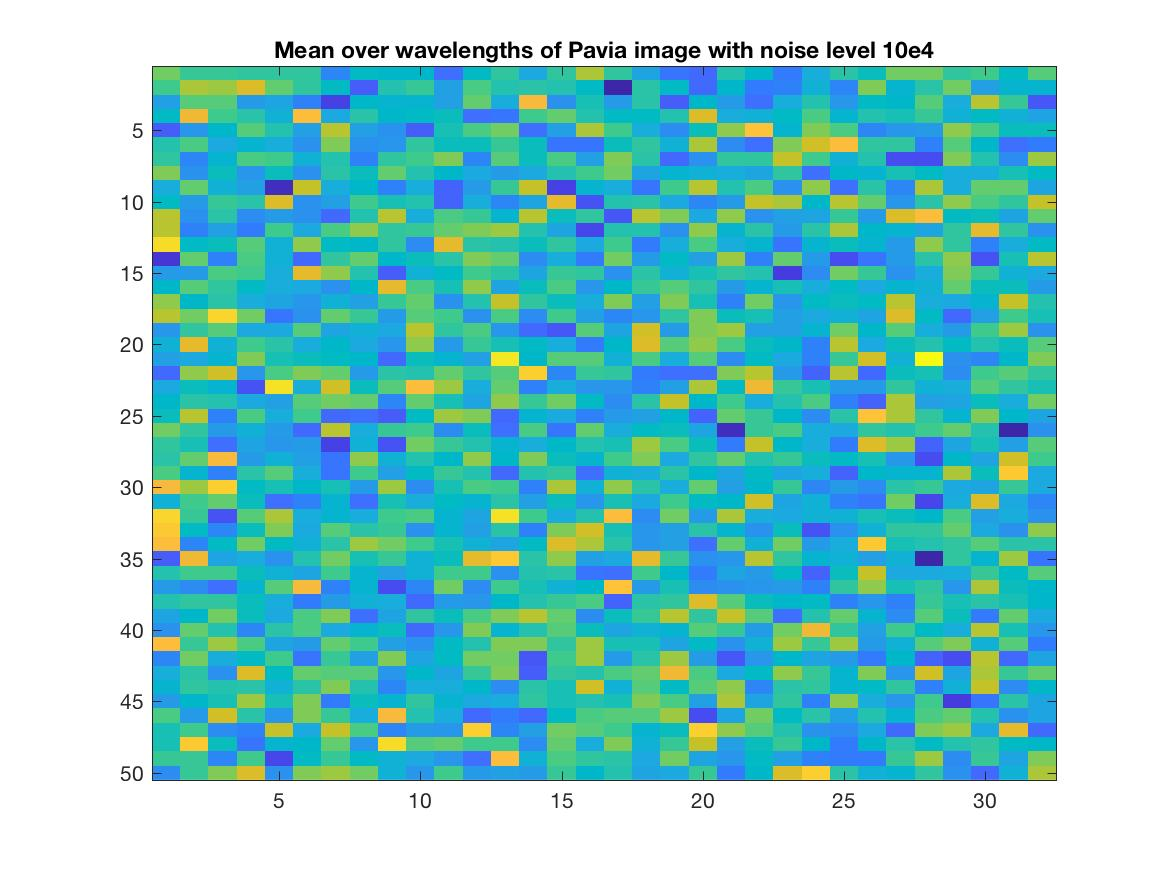
\includegraphics[width=.18\linewidth]{mean4.jpg}}}	
	\caption{Mean over all bands after adding noise for fake Pavia image}
	\label{Paviamean}
\end{figure}

\begin{figure}[H]
	\centering
	\subfloat{{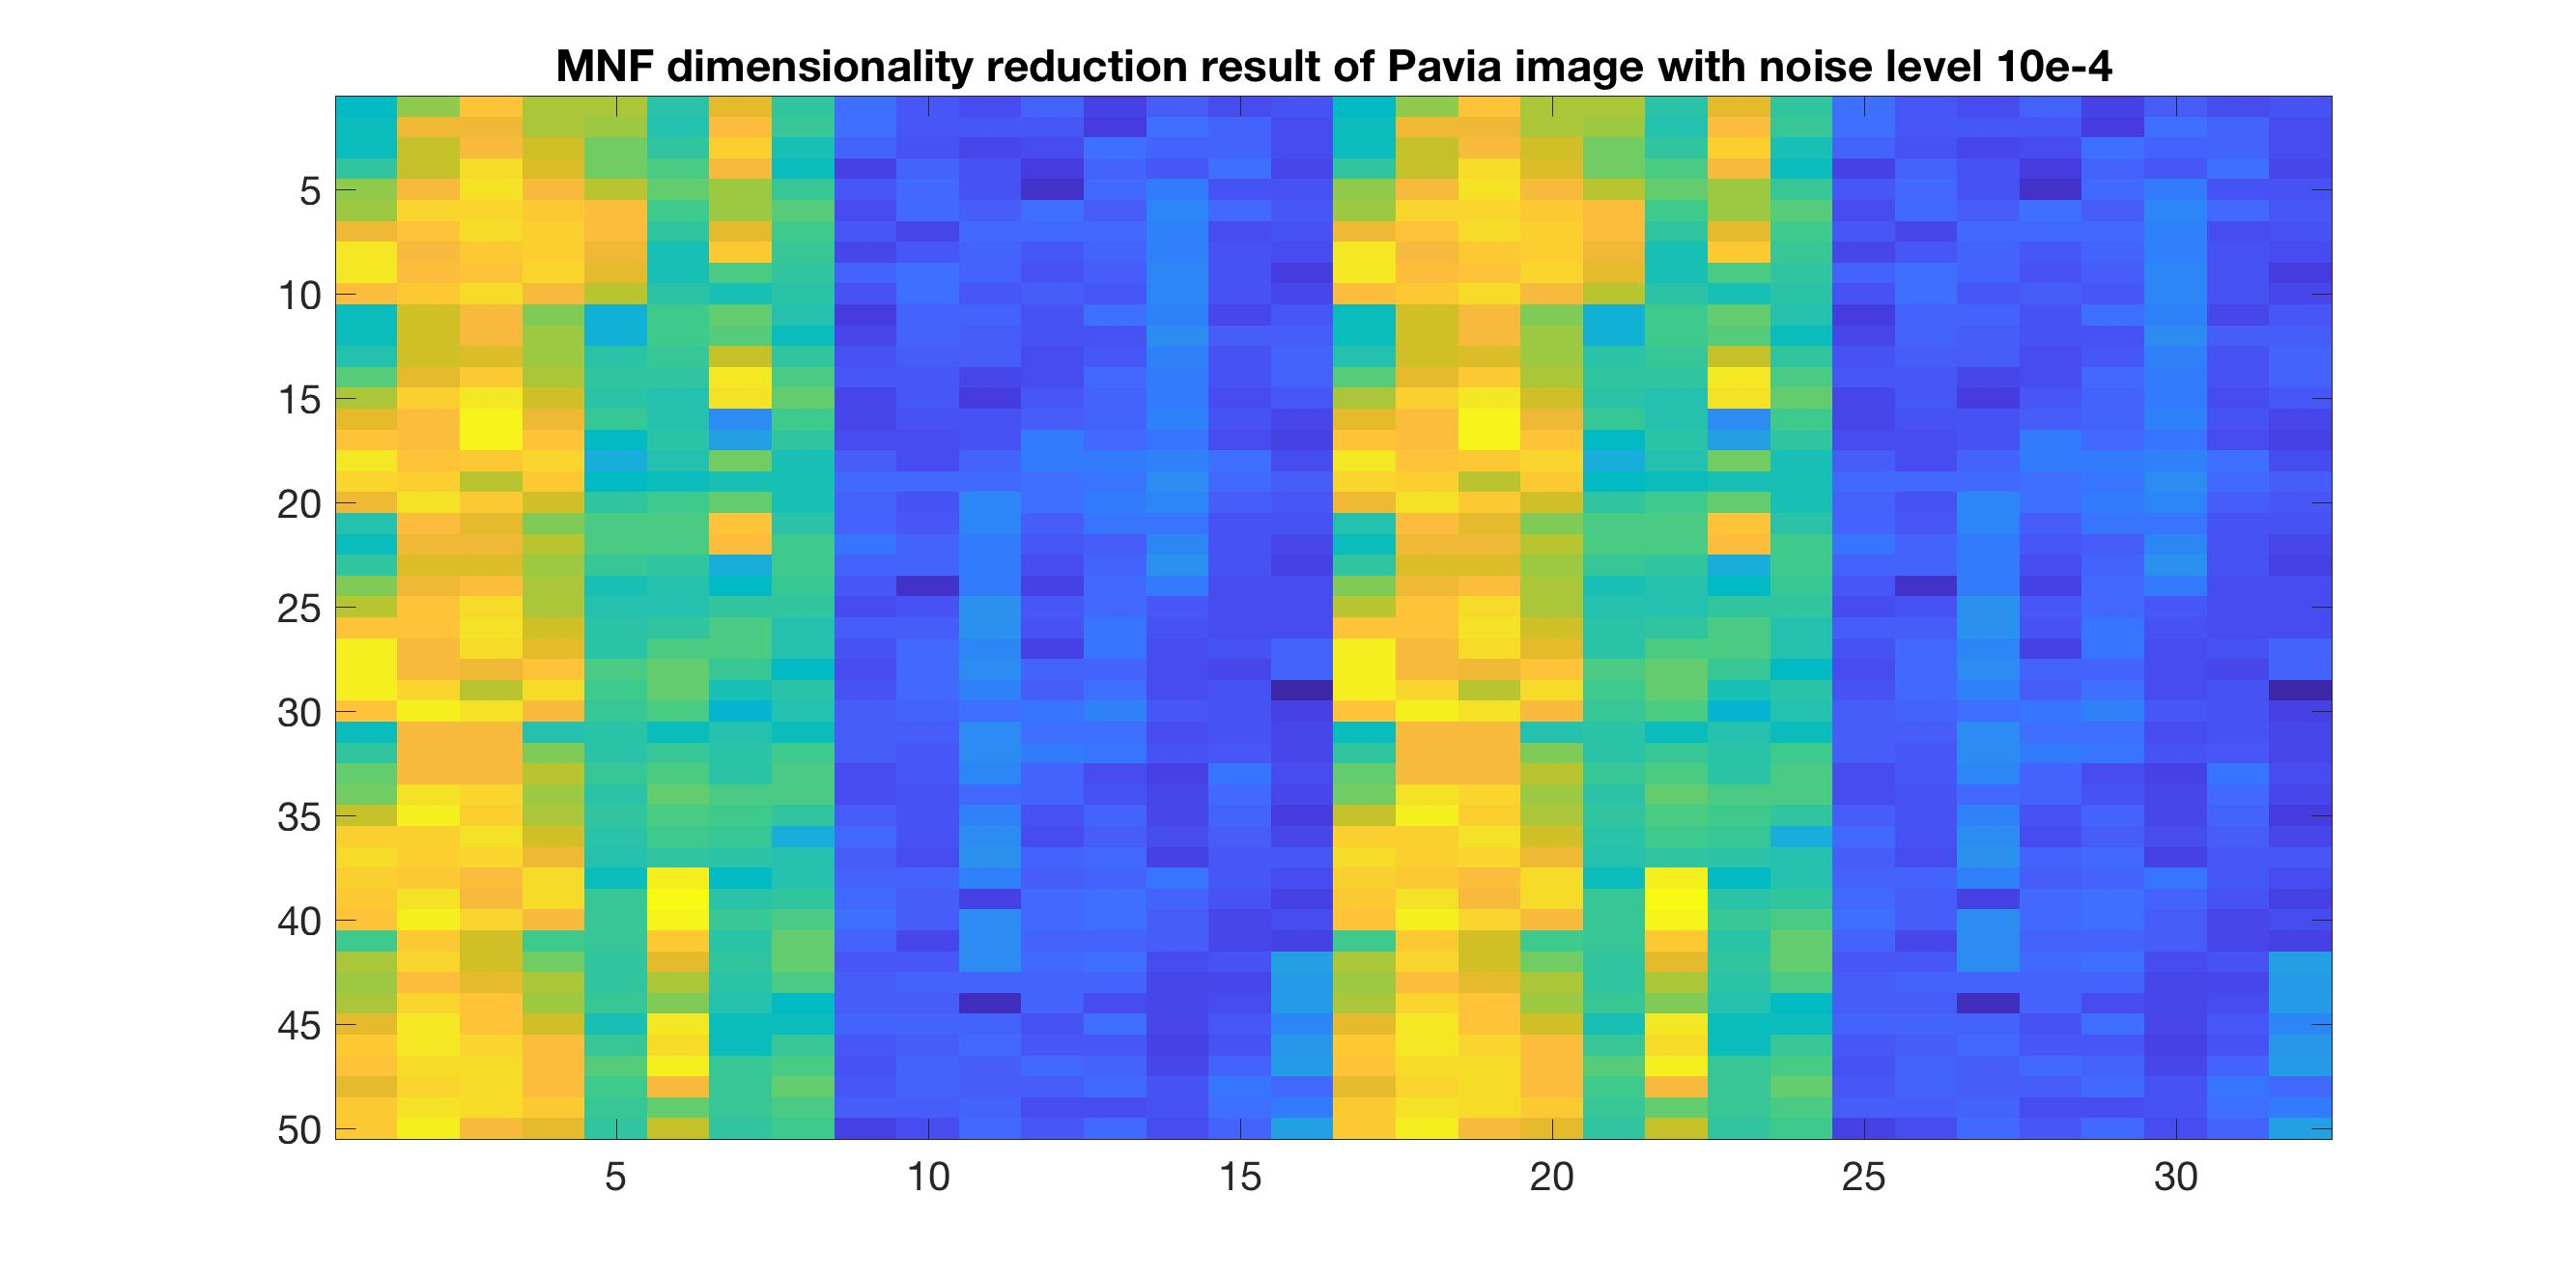
\includegraphics[width=.18\linewidth]{mnf-4.jpg}}}
	\subfloat{{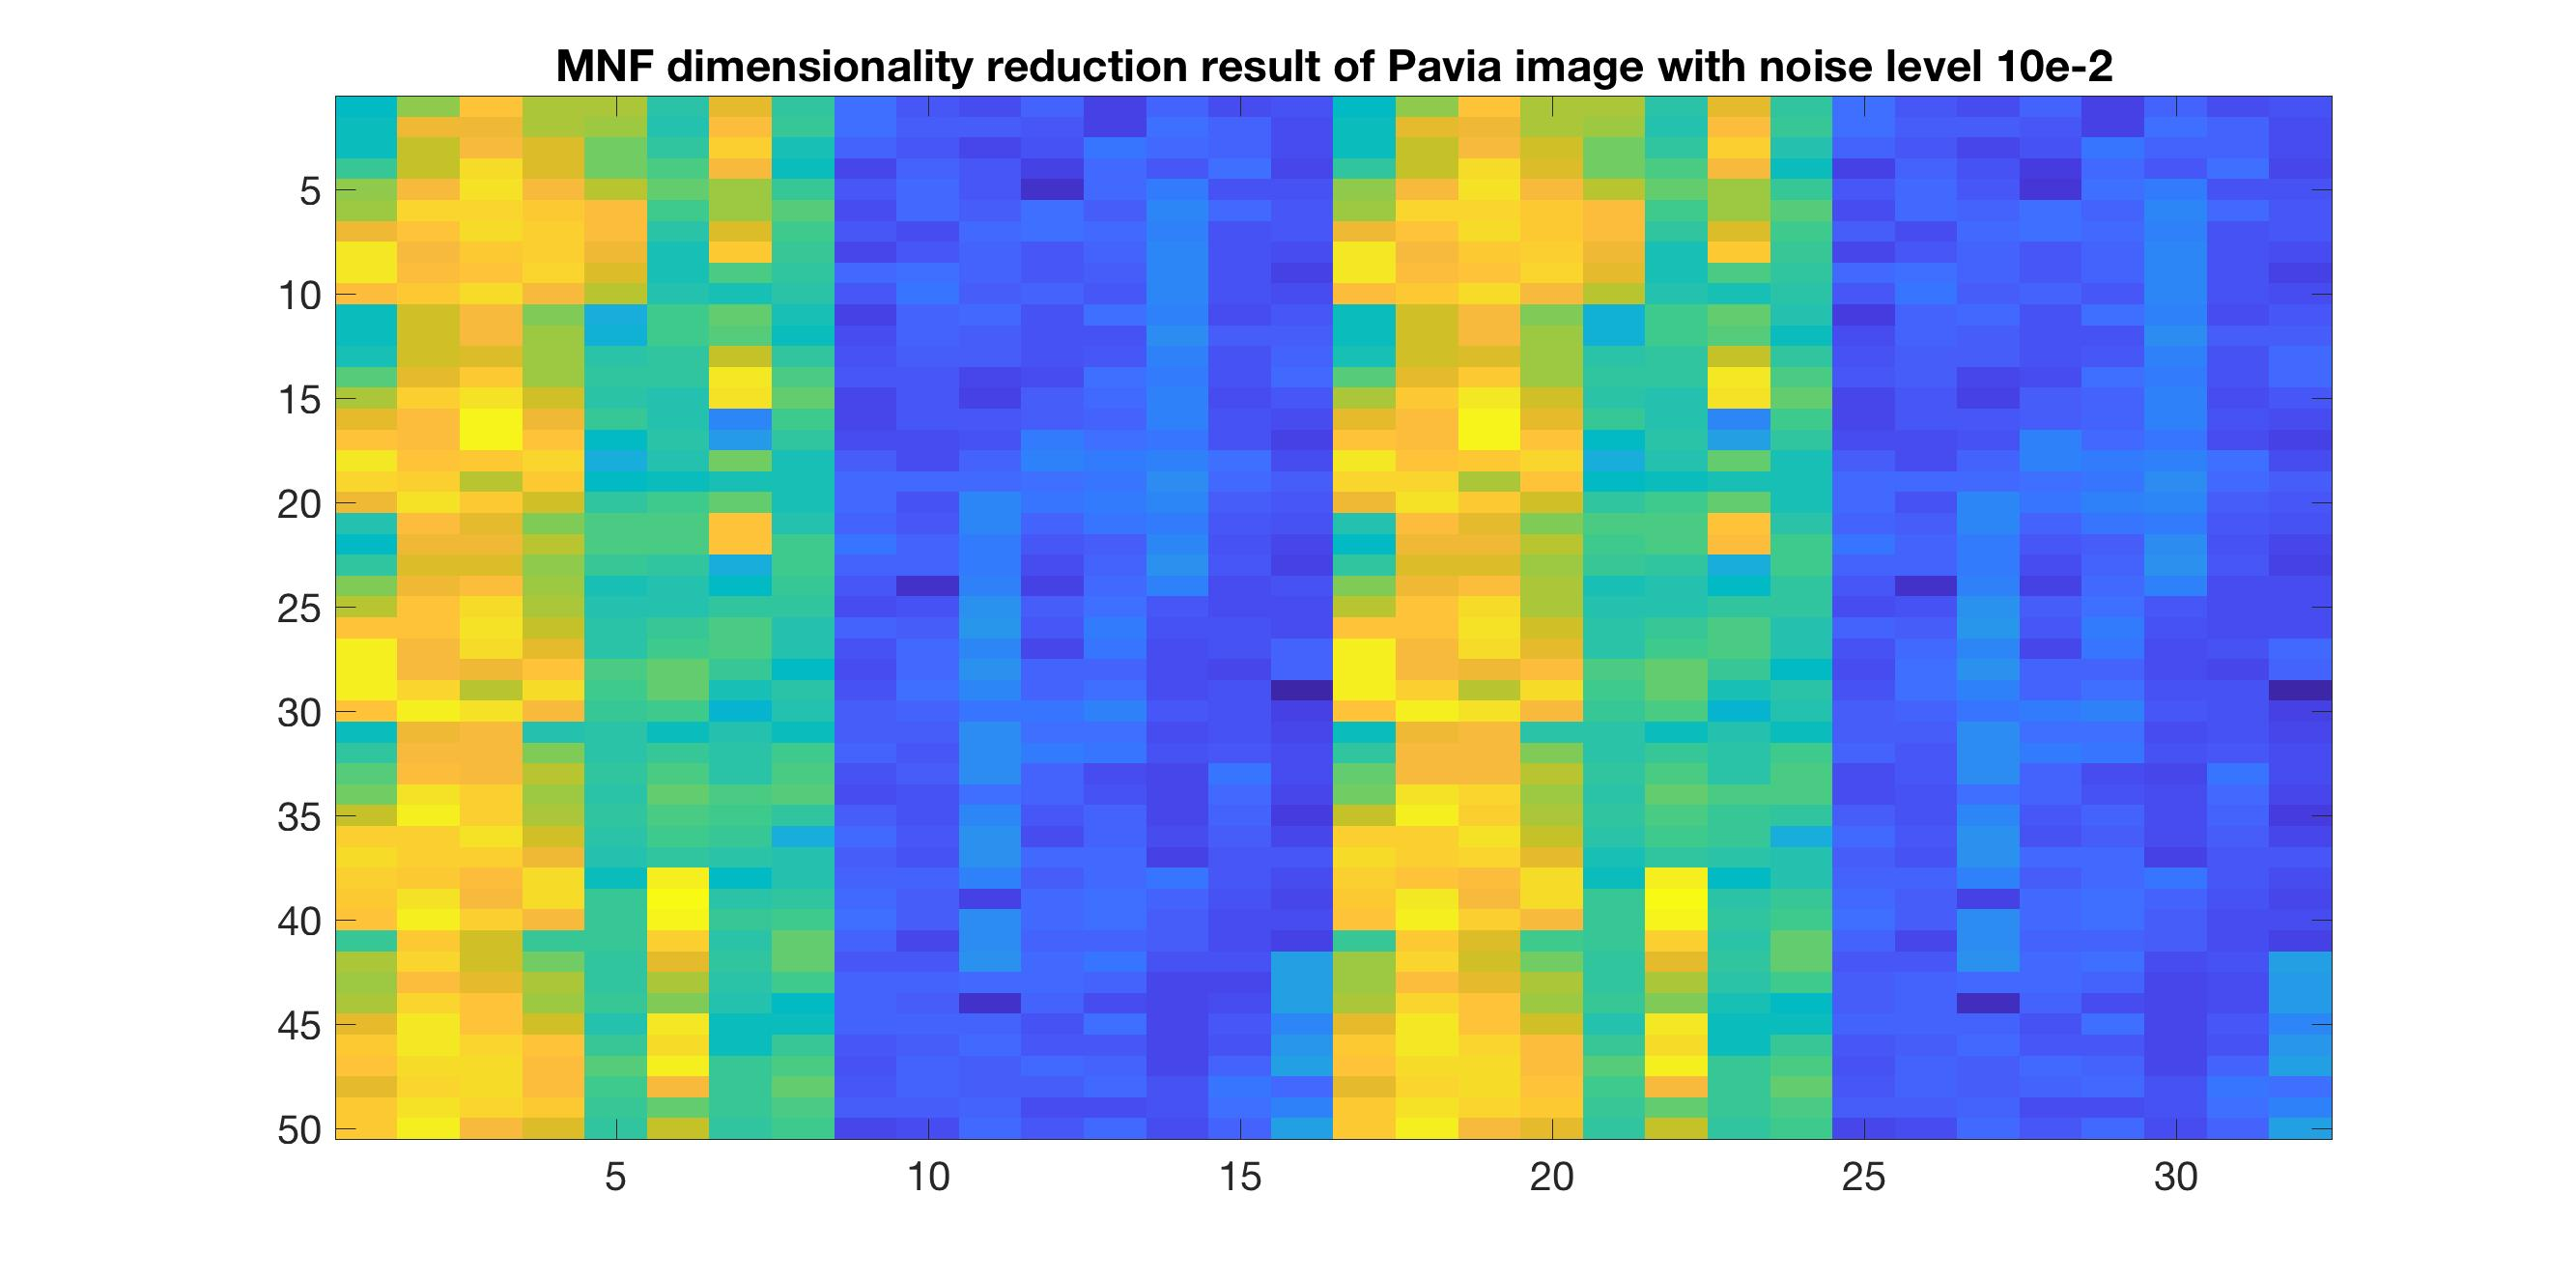
\includegraphics[width=.18\linewidth]{mnf-2.jpg}}}	
	\subfloat{{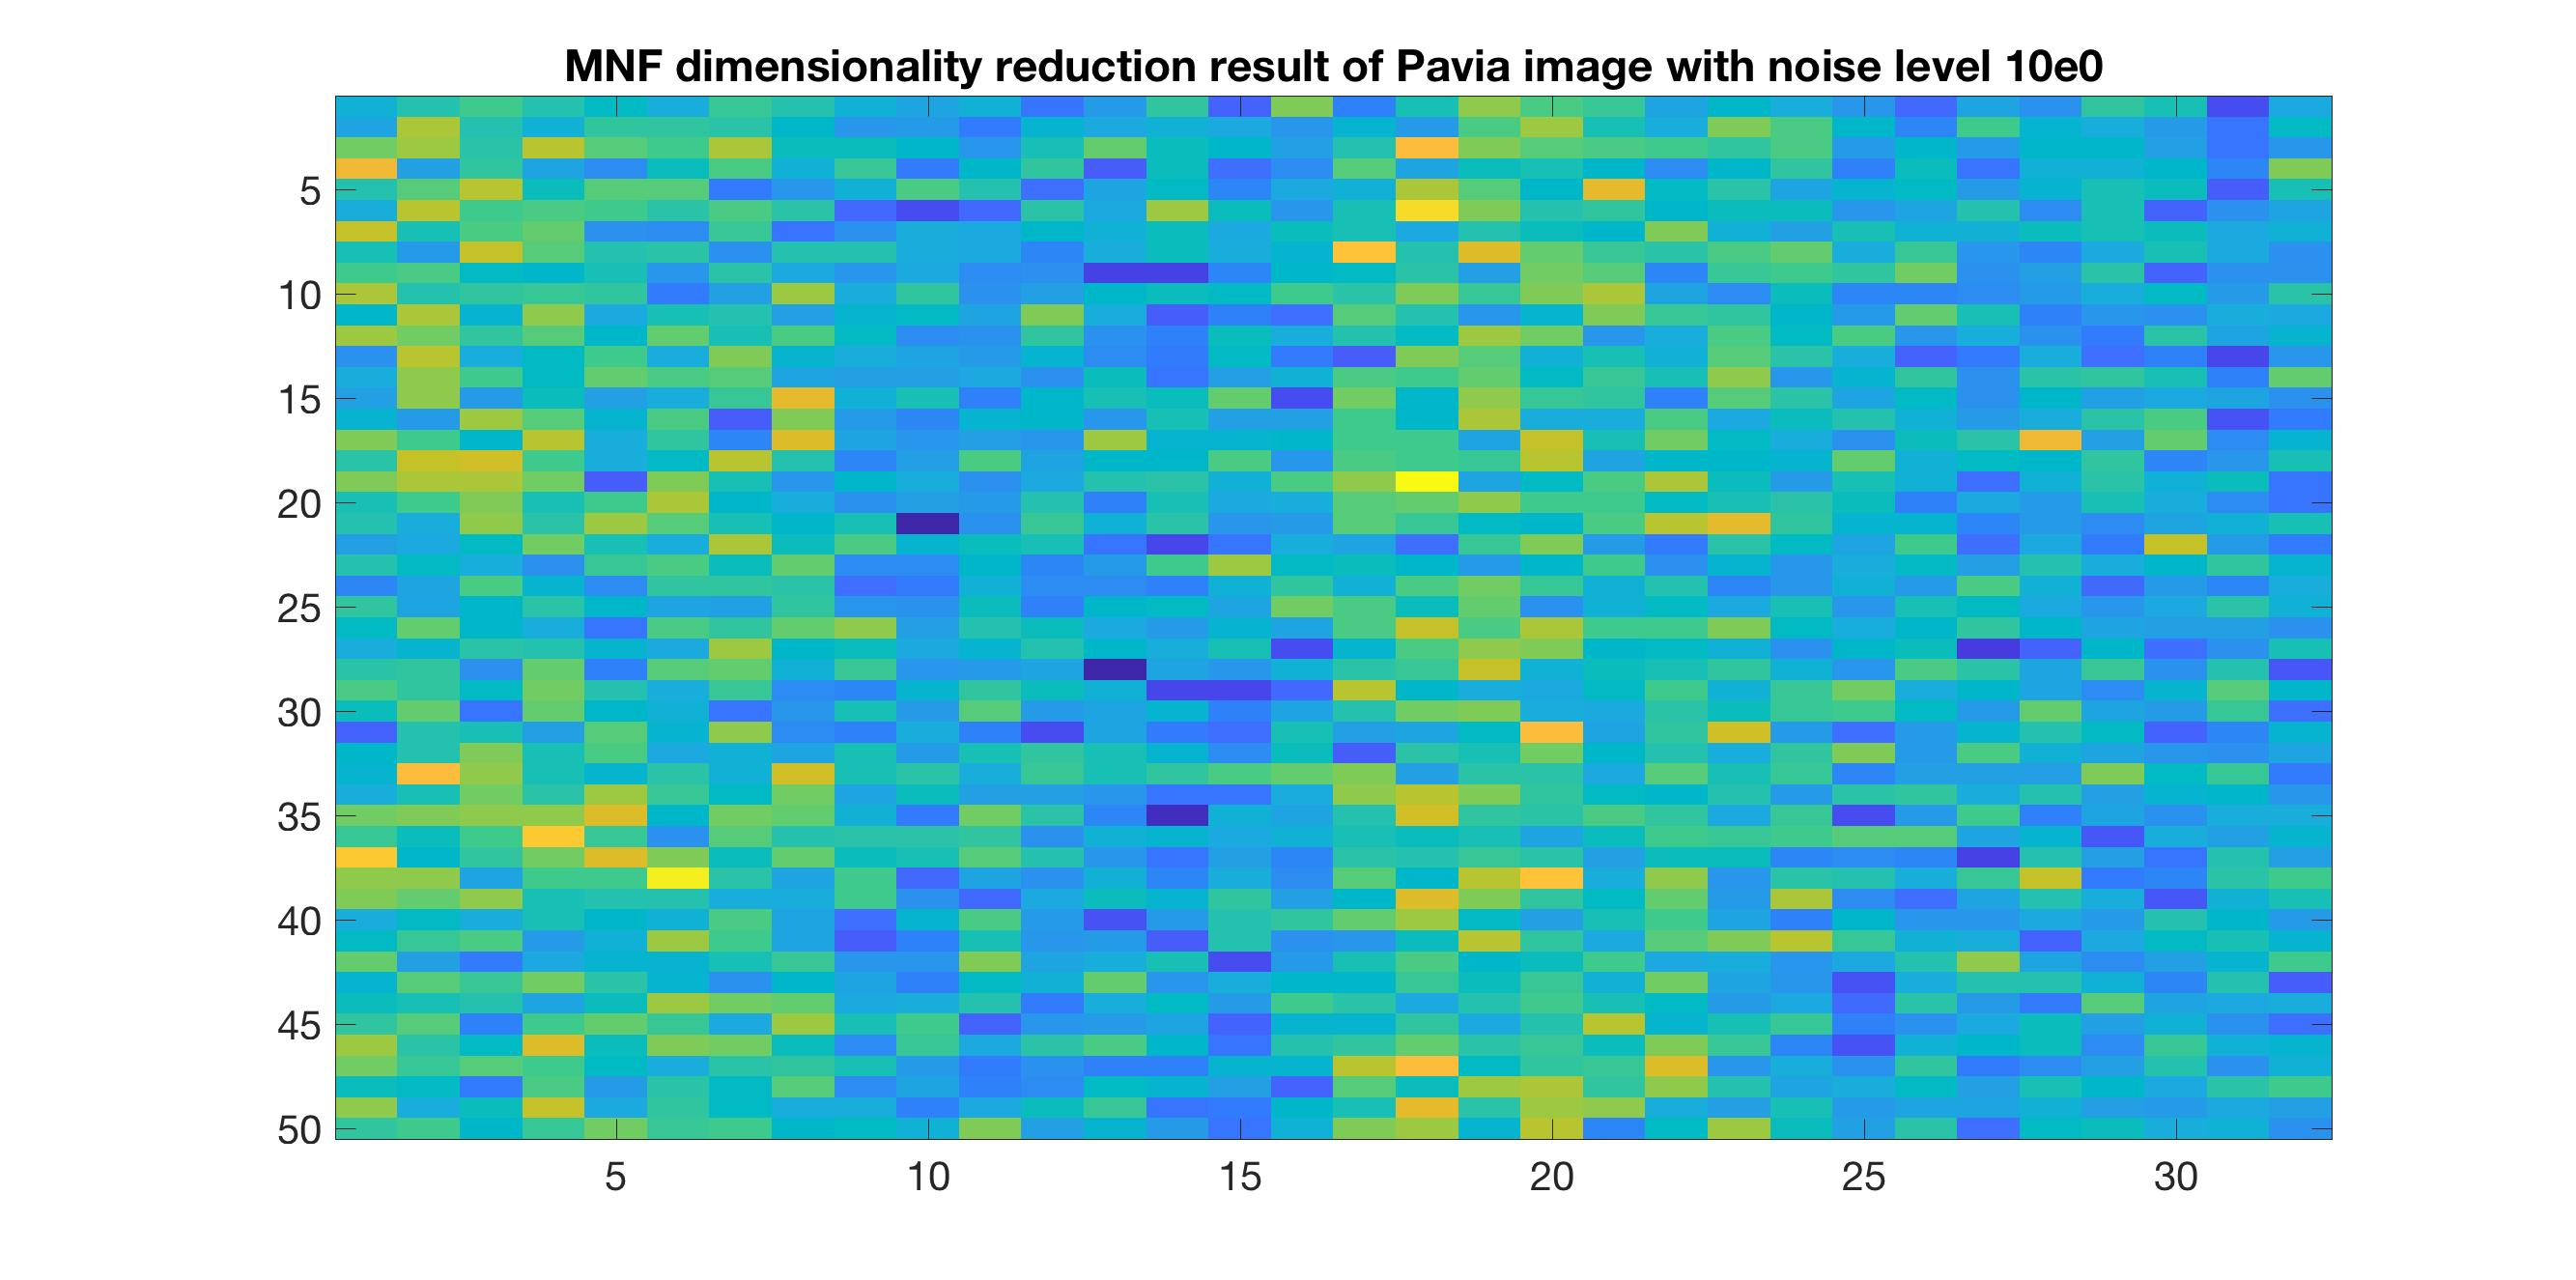
\includegraphics[width=.18\linewidth]{mnf0.jpg}}}	
	\subfloat{{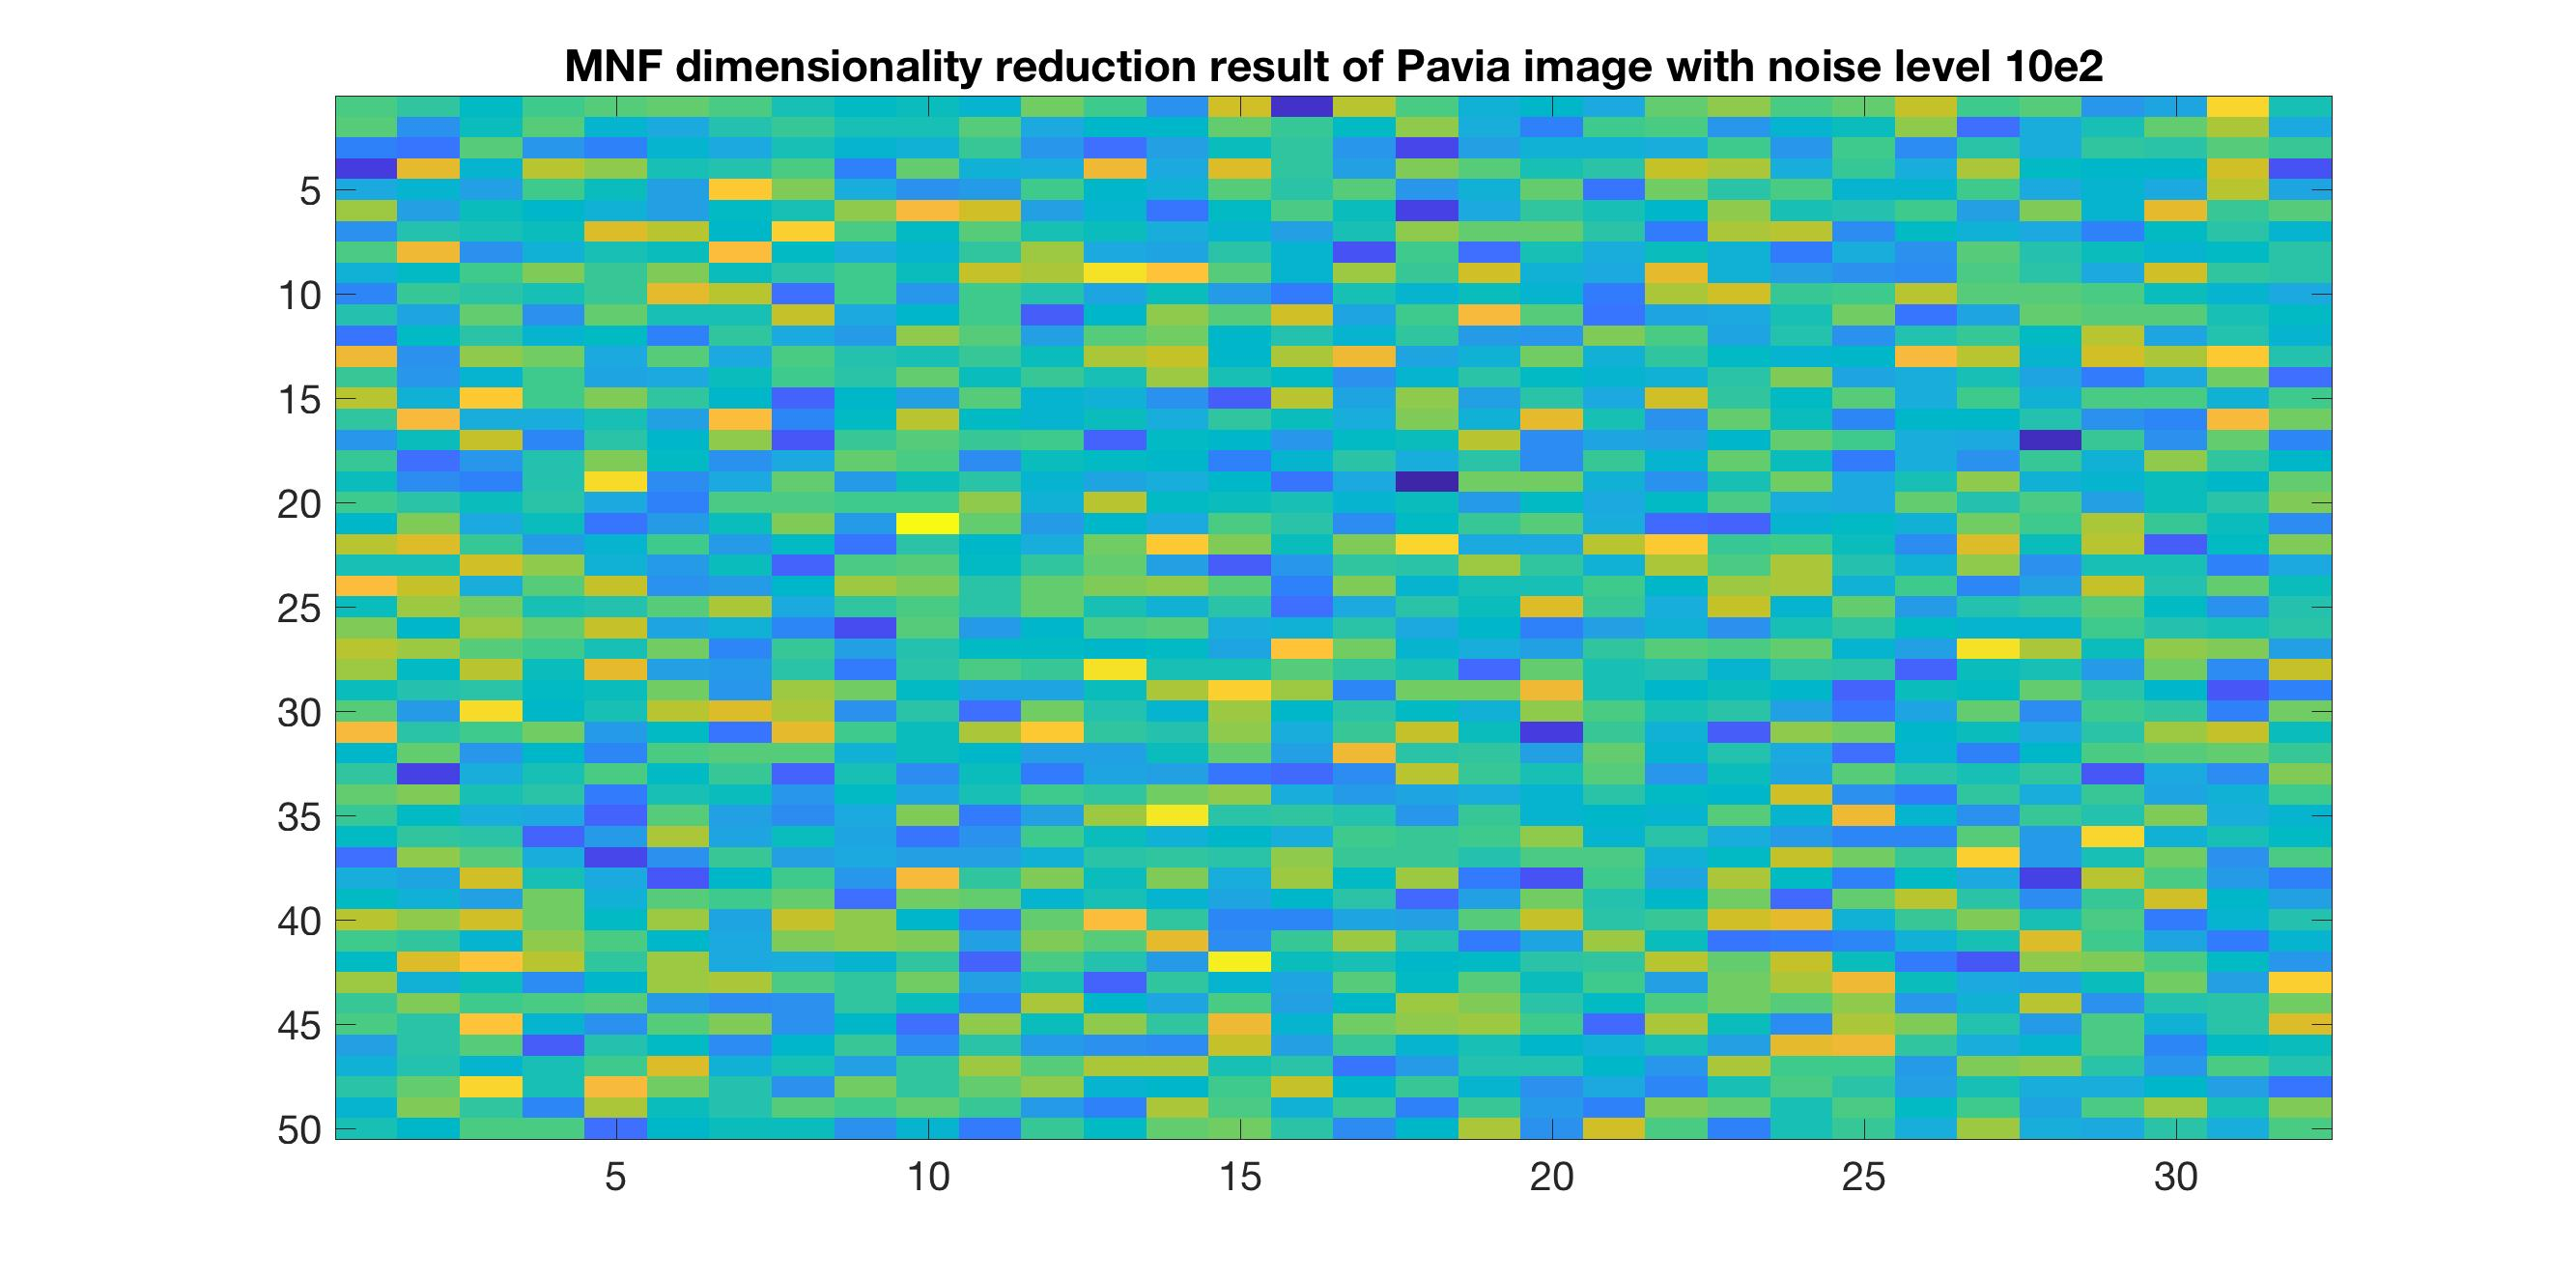
\includegraphics[width=.18\linewidth]{mnf2.jpg}}}	
	\subfloat{{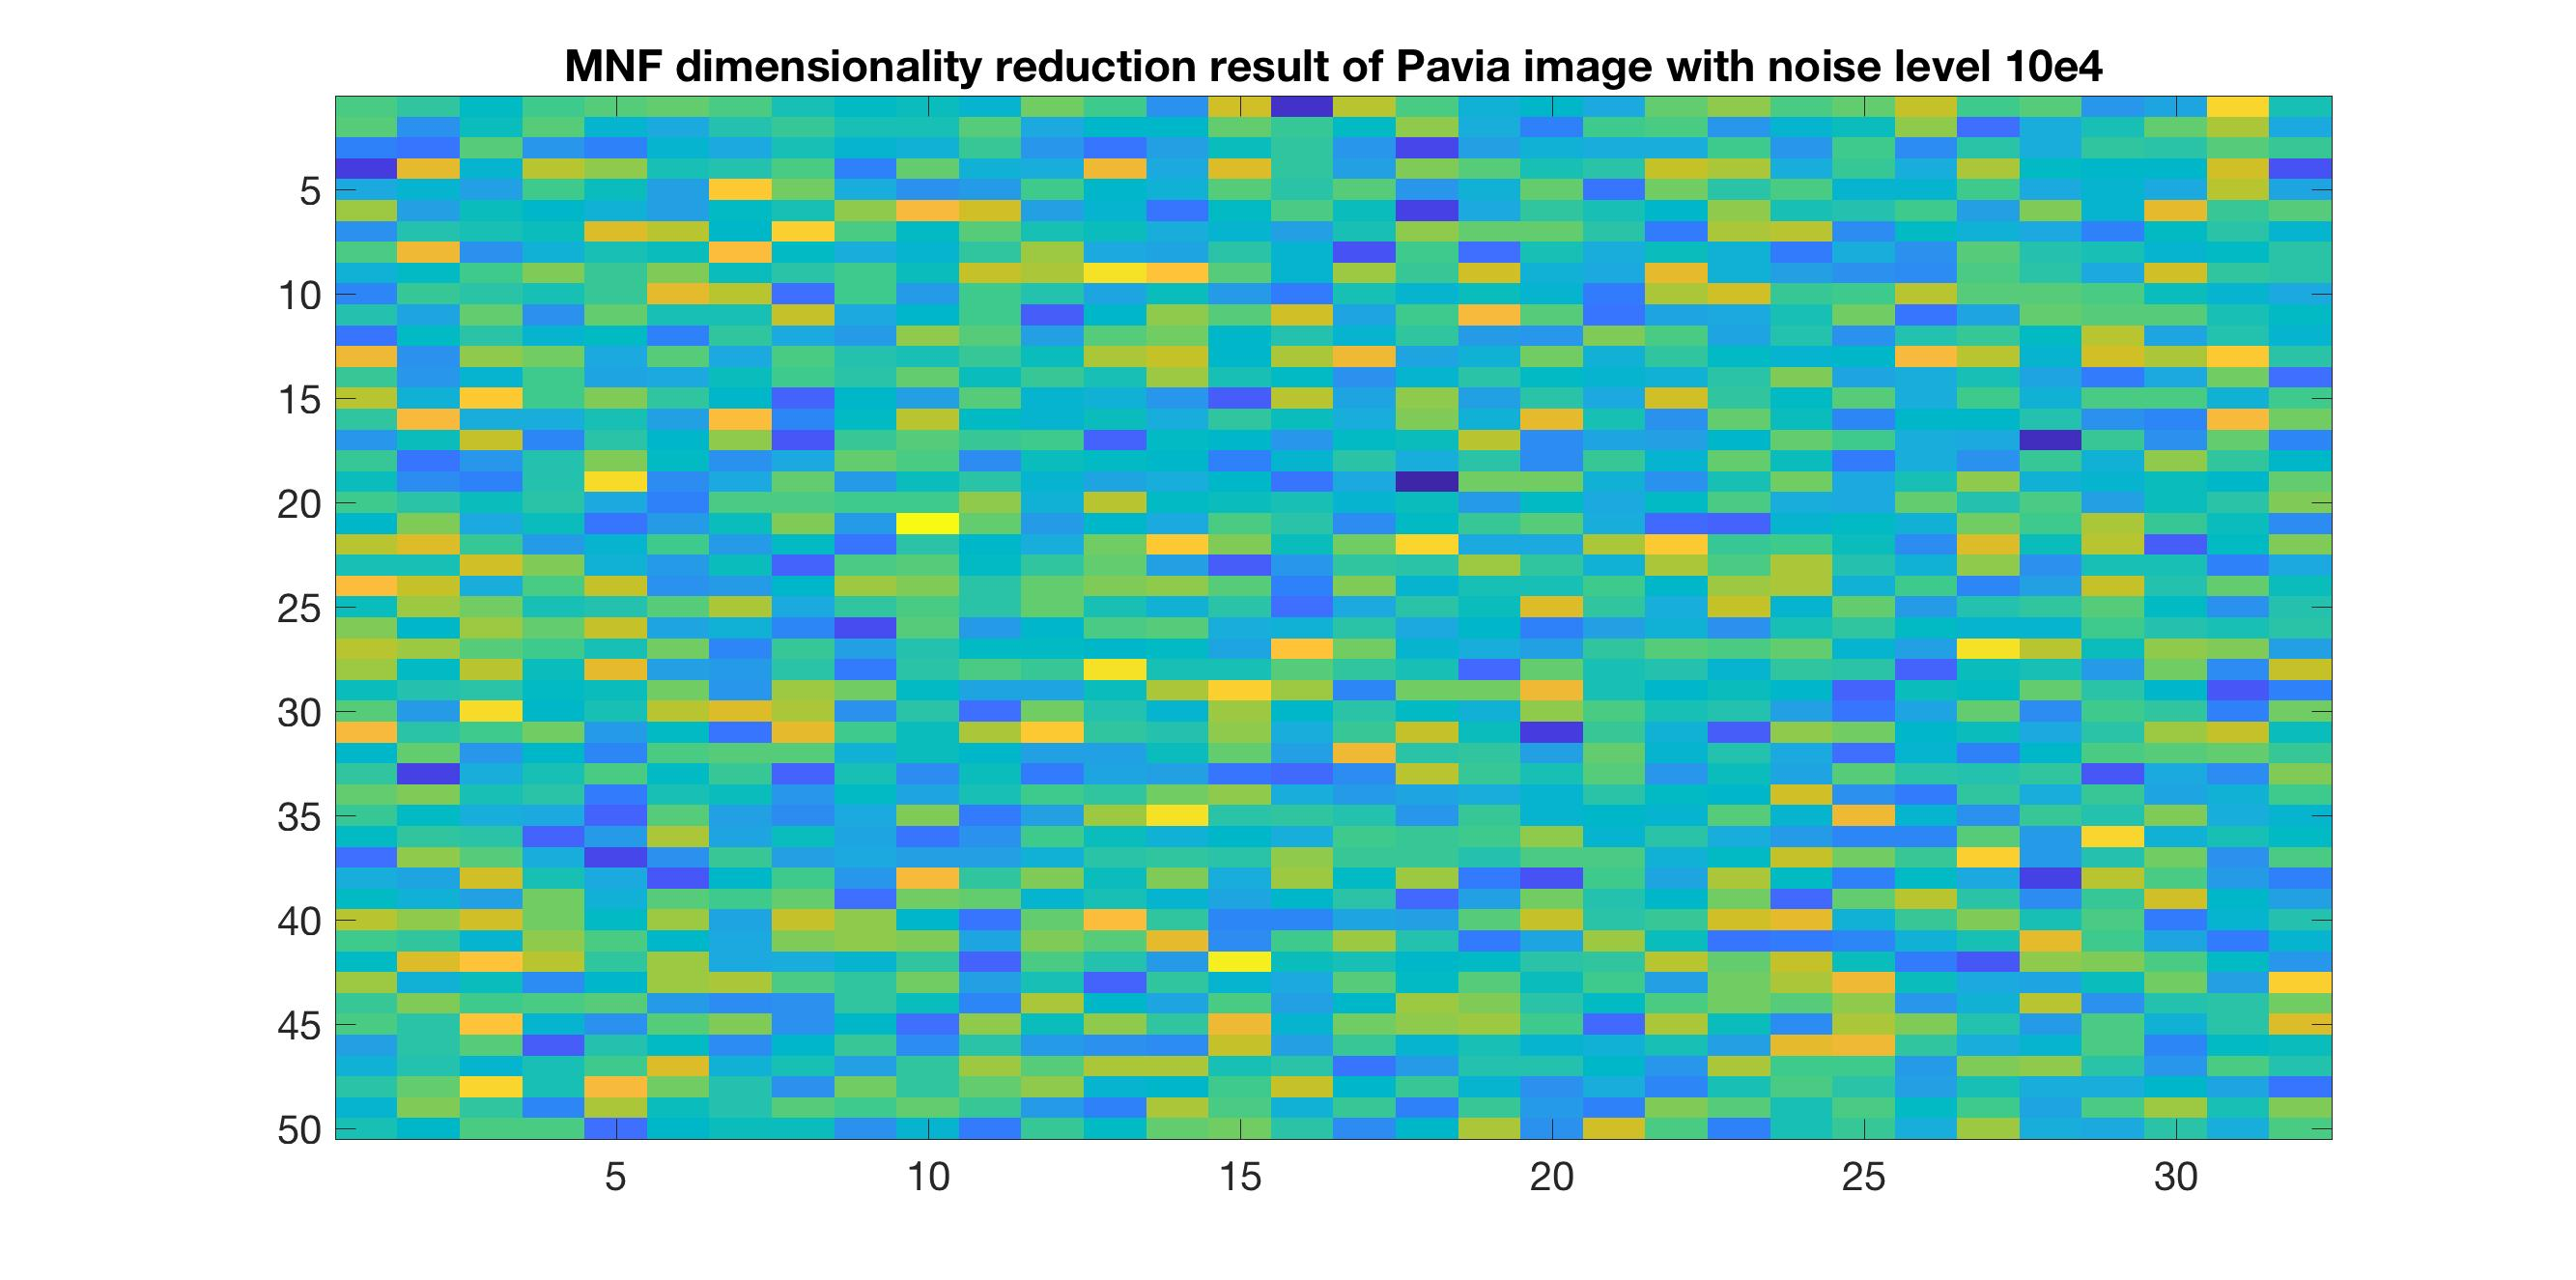
\includegraphics[width=.18\linewidth]{mnf4.jpg}}}	
	\caption{Mean over all bands after MNF dimensionality reduction with noise added  to the fake Pavia image}
	\label{Paviamnfmean}
\end{figure}

\begin{figure}[H]
	\centering
	\subfloat{{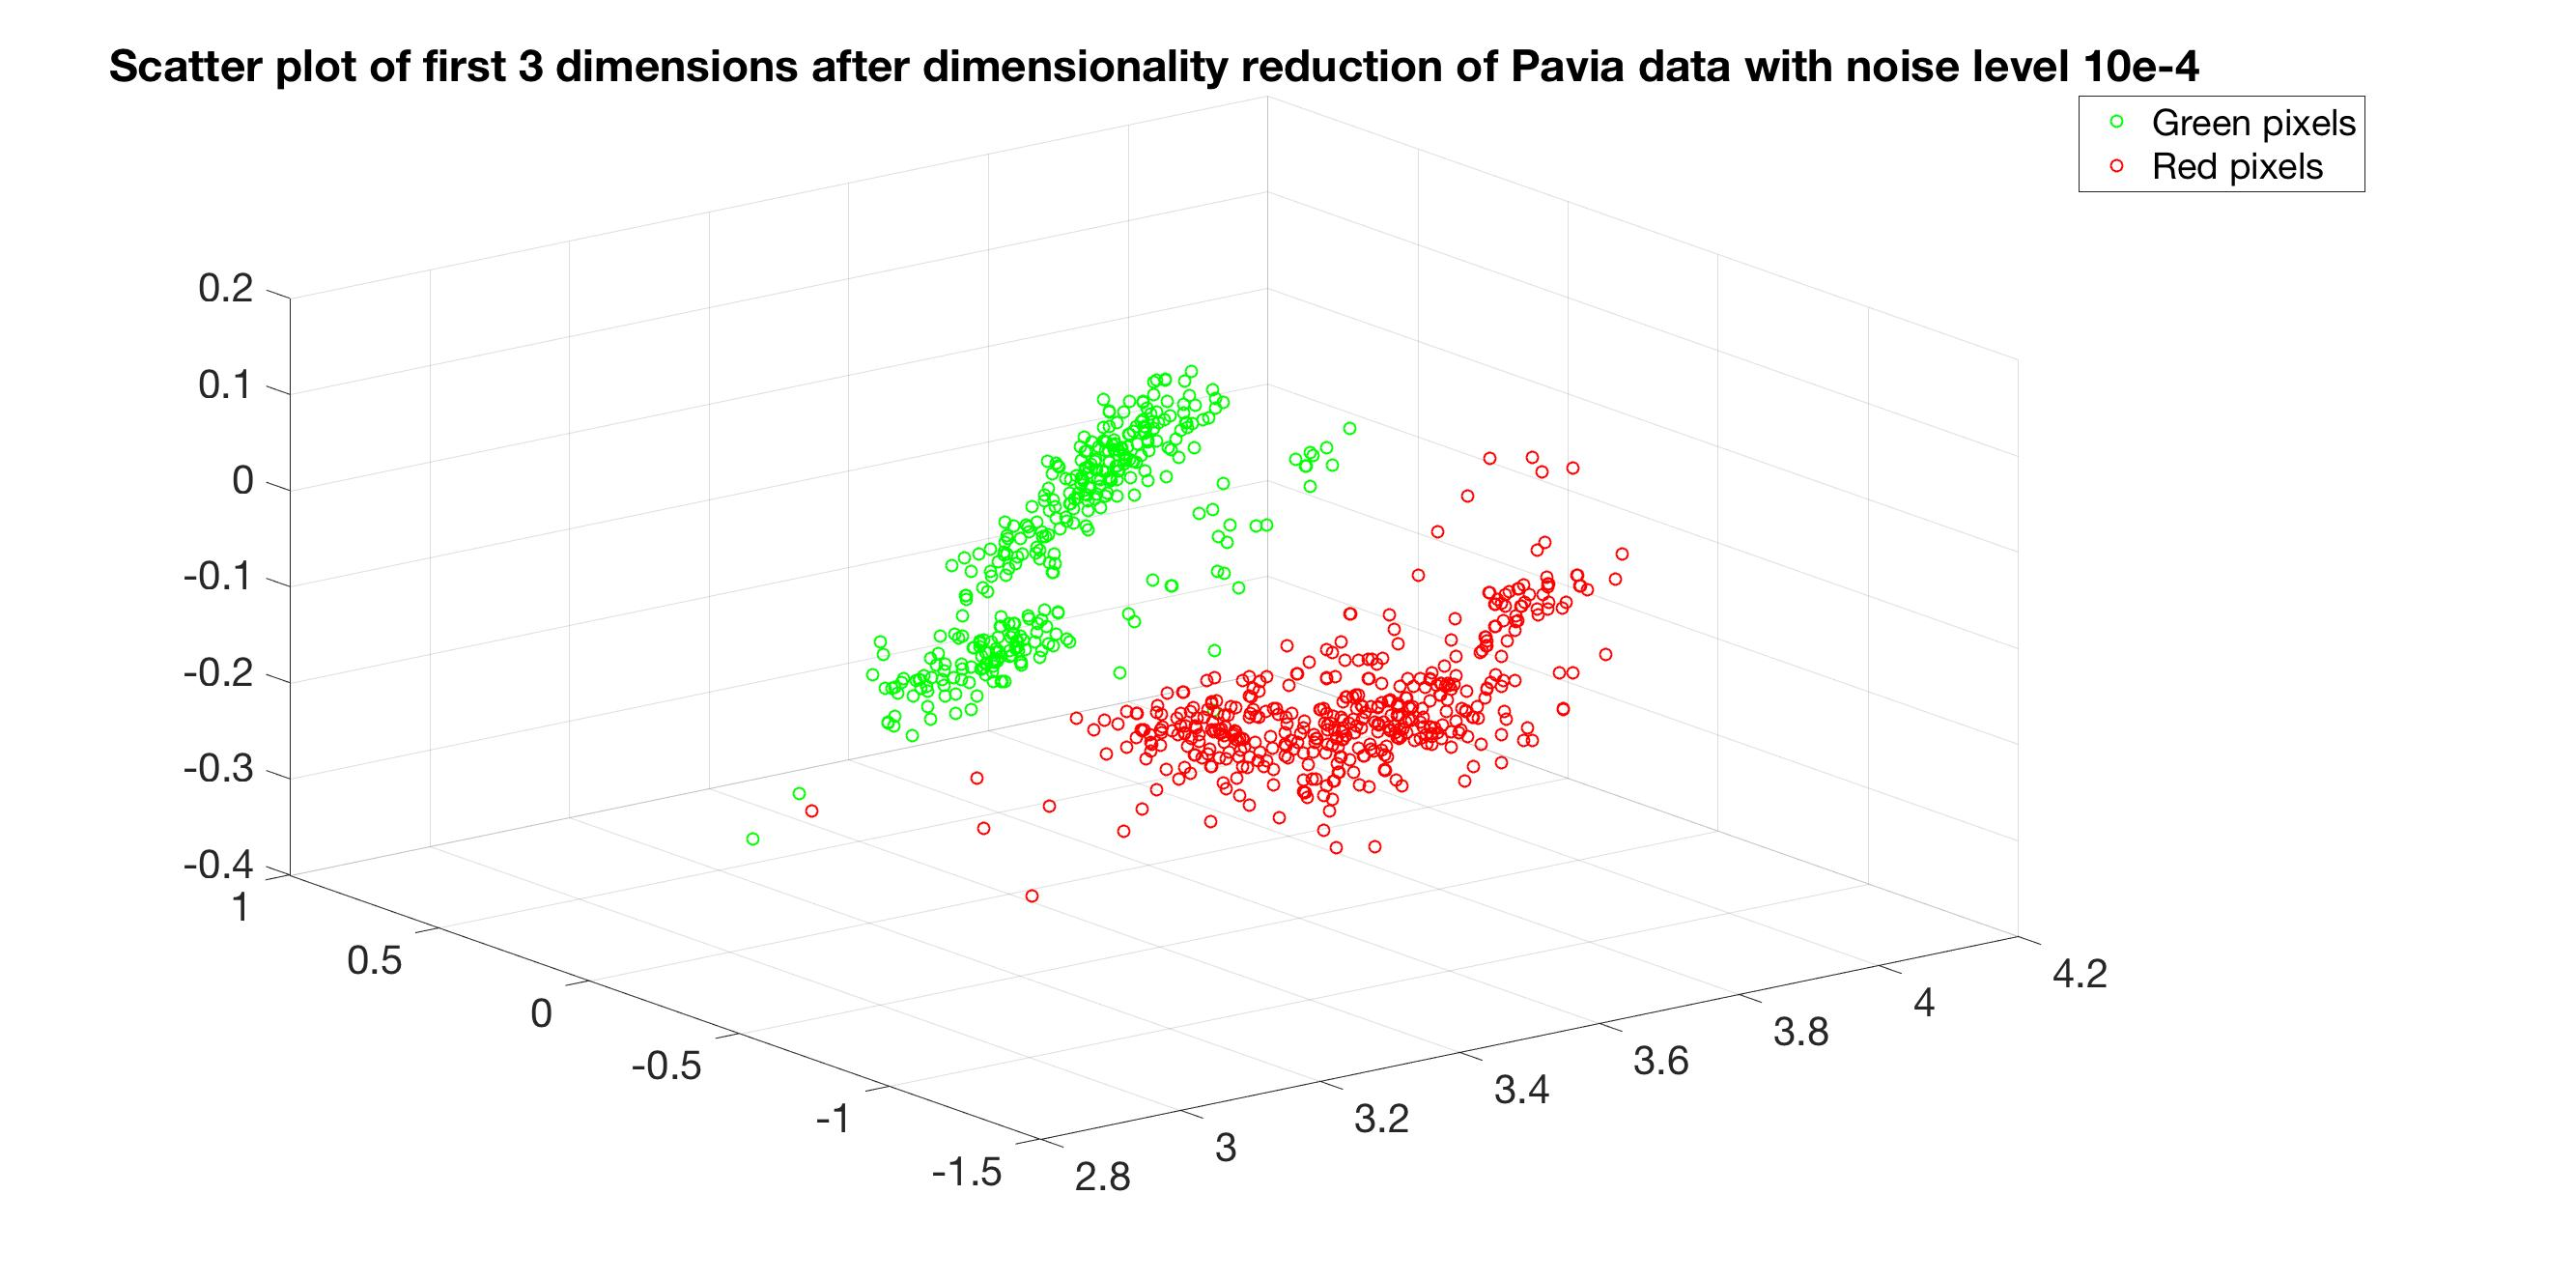
\includegraphics[width=.18\linewidth]{Noisescattermnf-4.jpg}}}
	\subfloat{{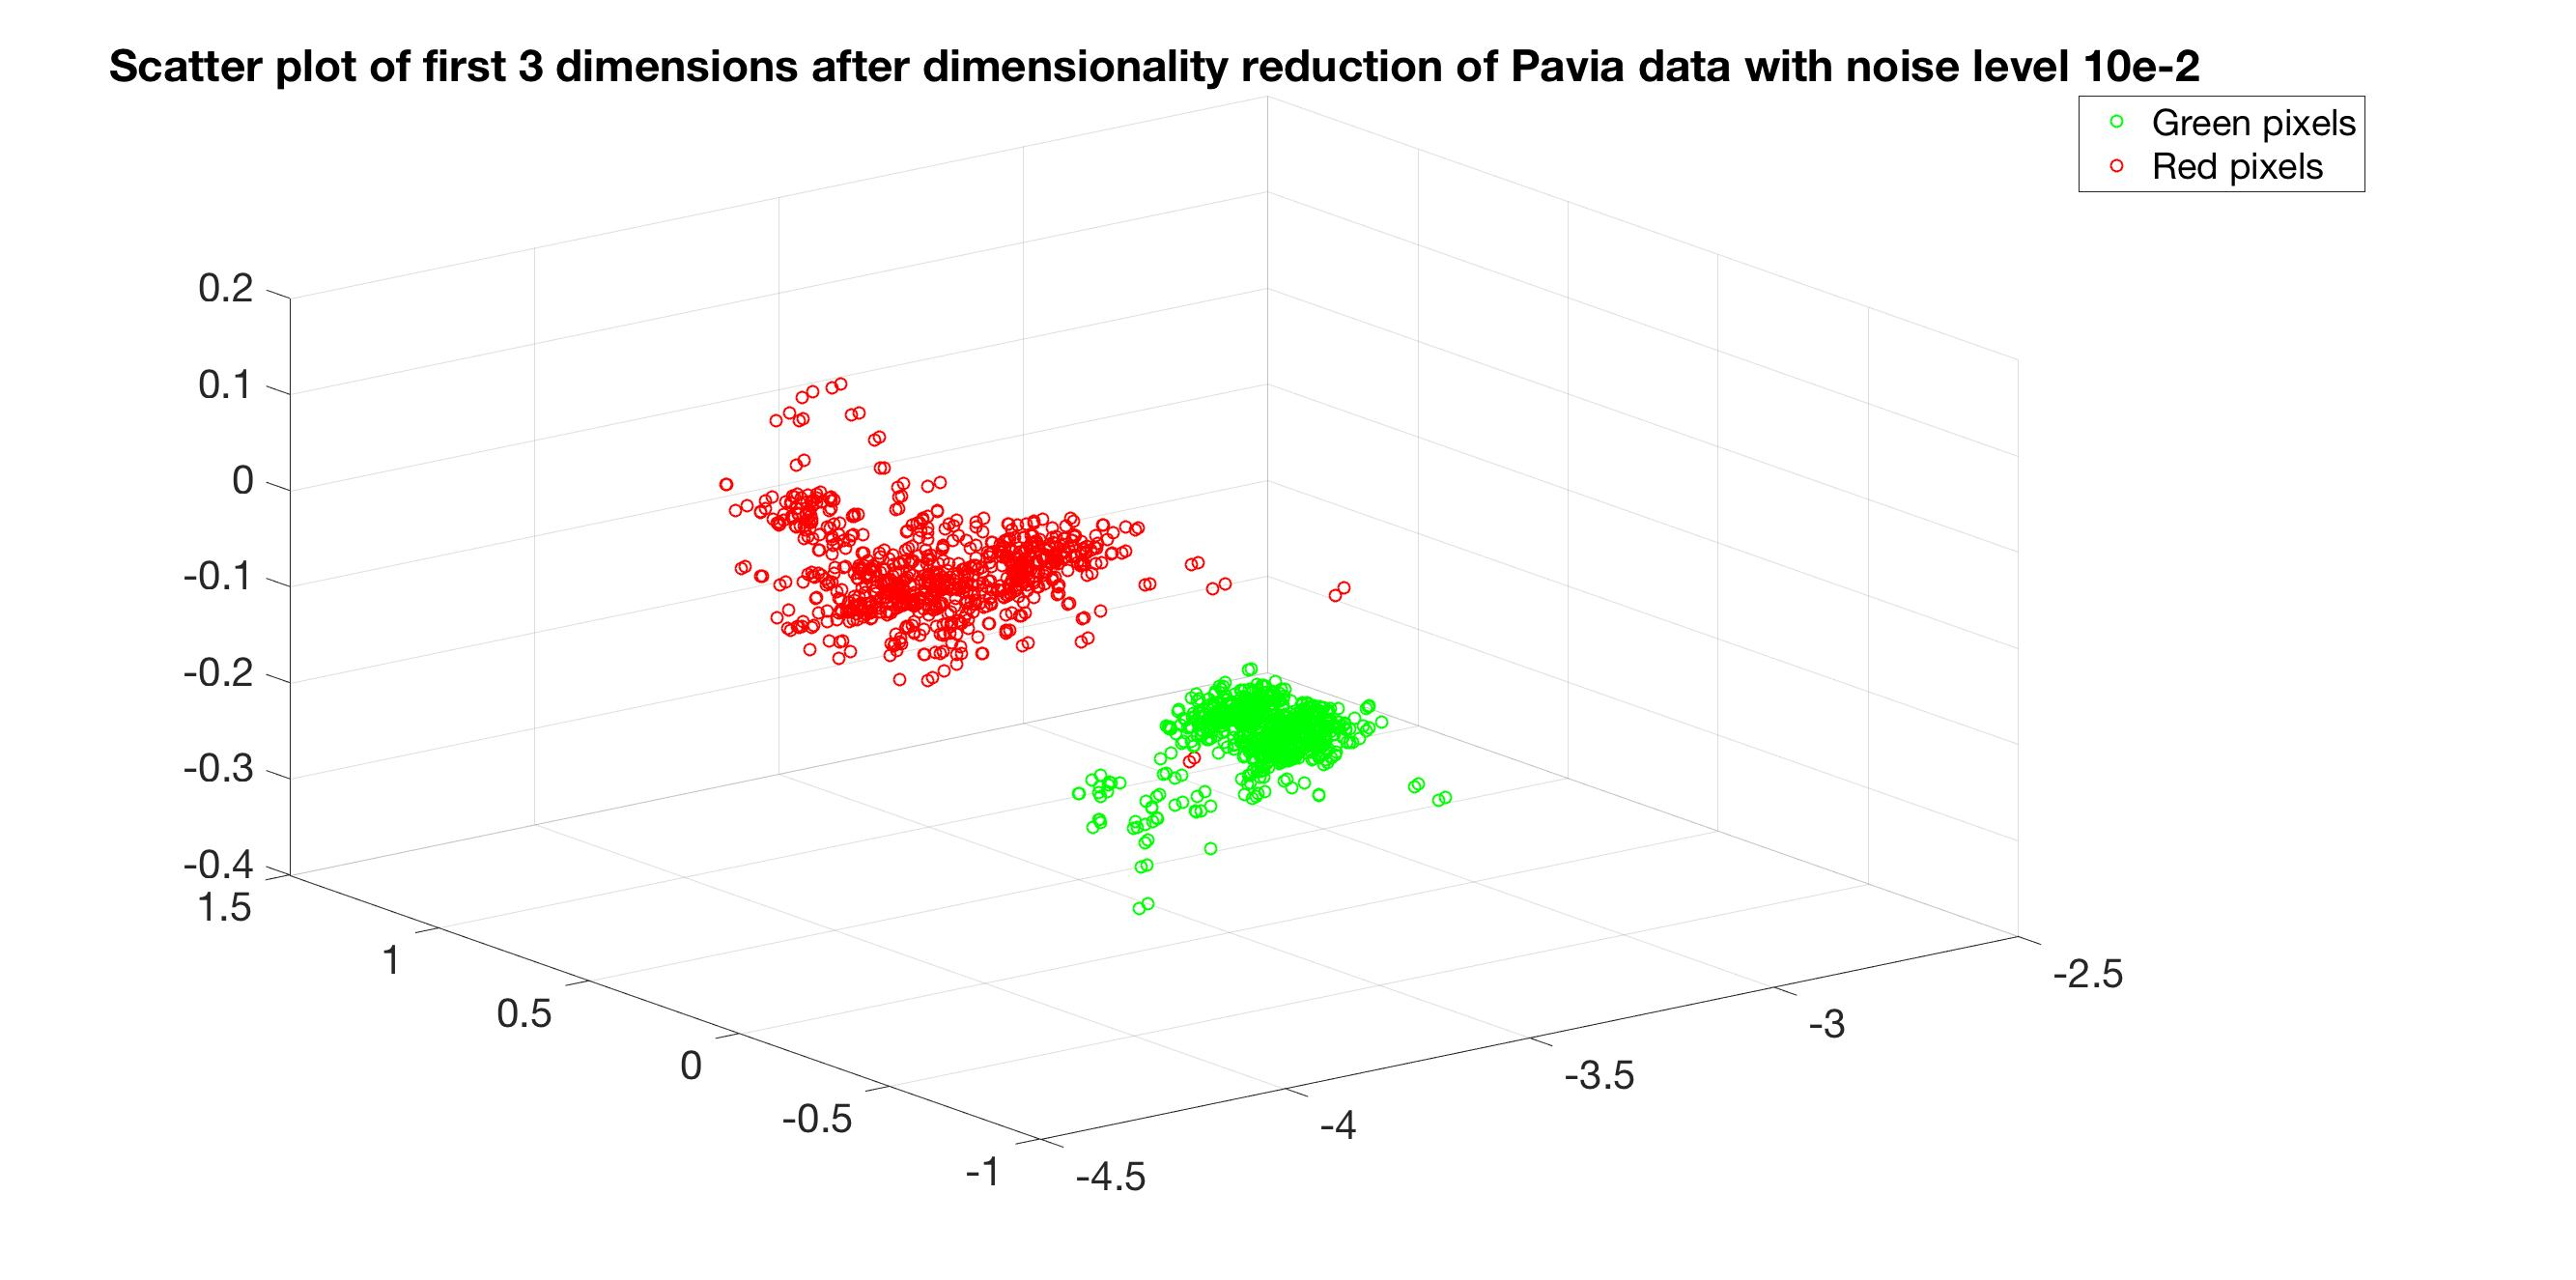
\includegraphics[width=.18\linewidth]{Noisescattermnf-2.jpg}}}	
	\subfloat{{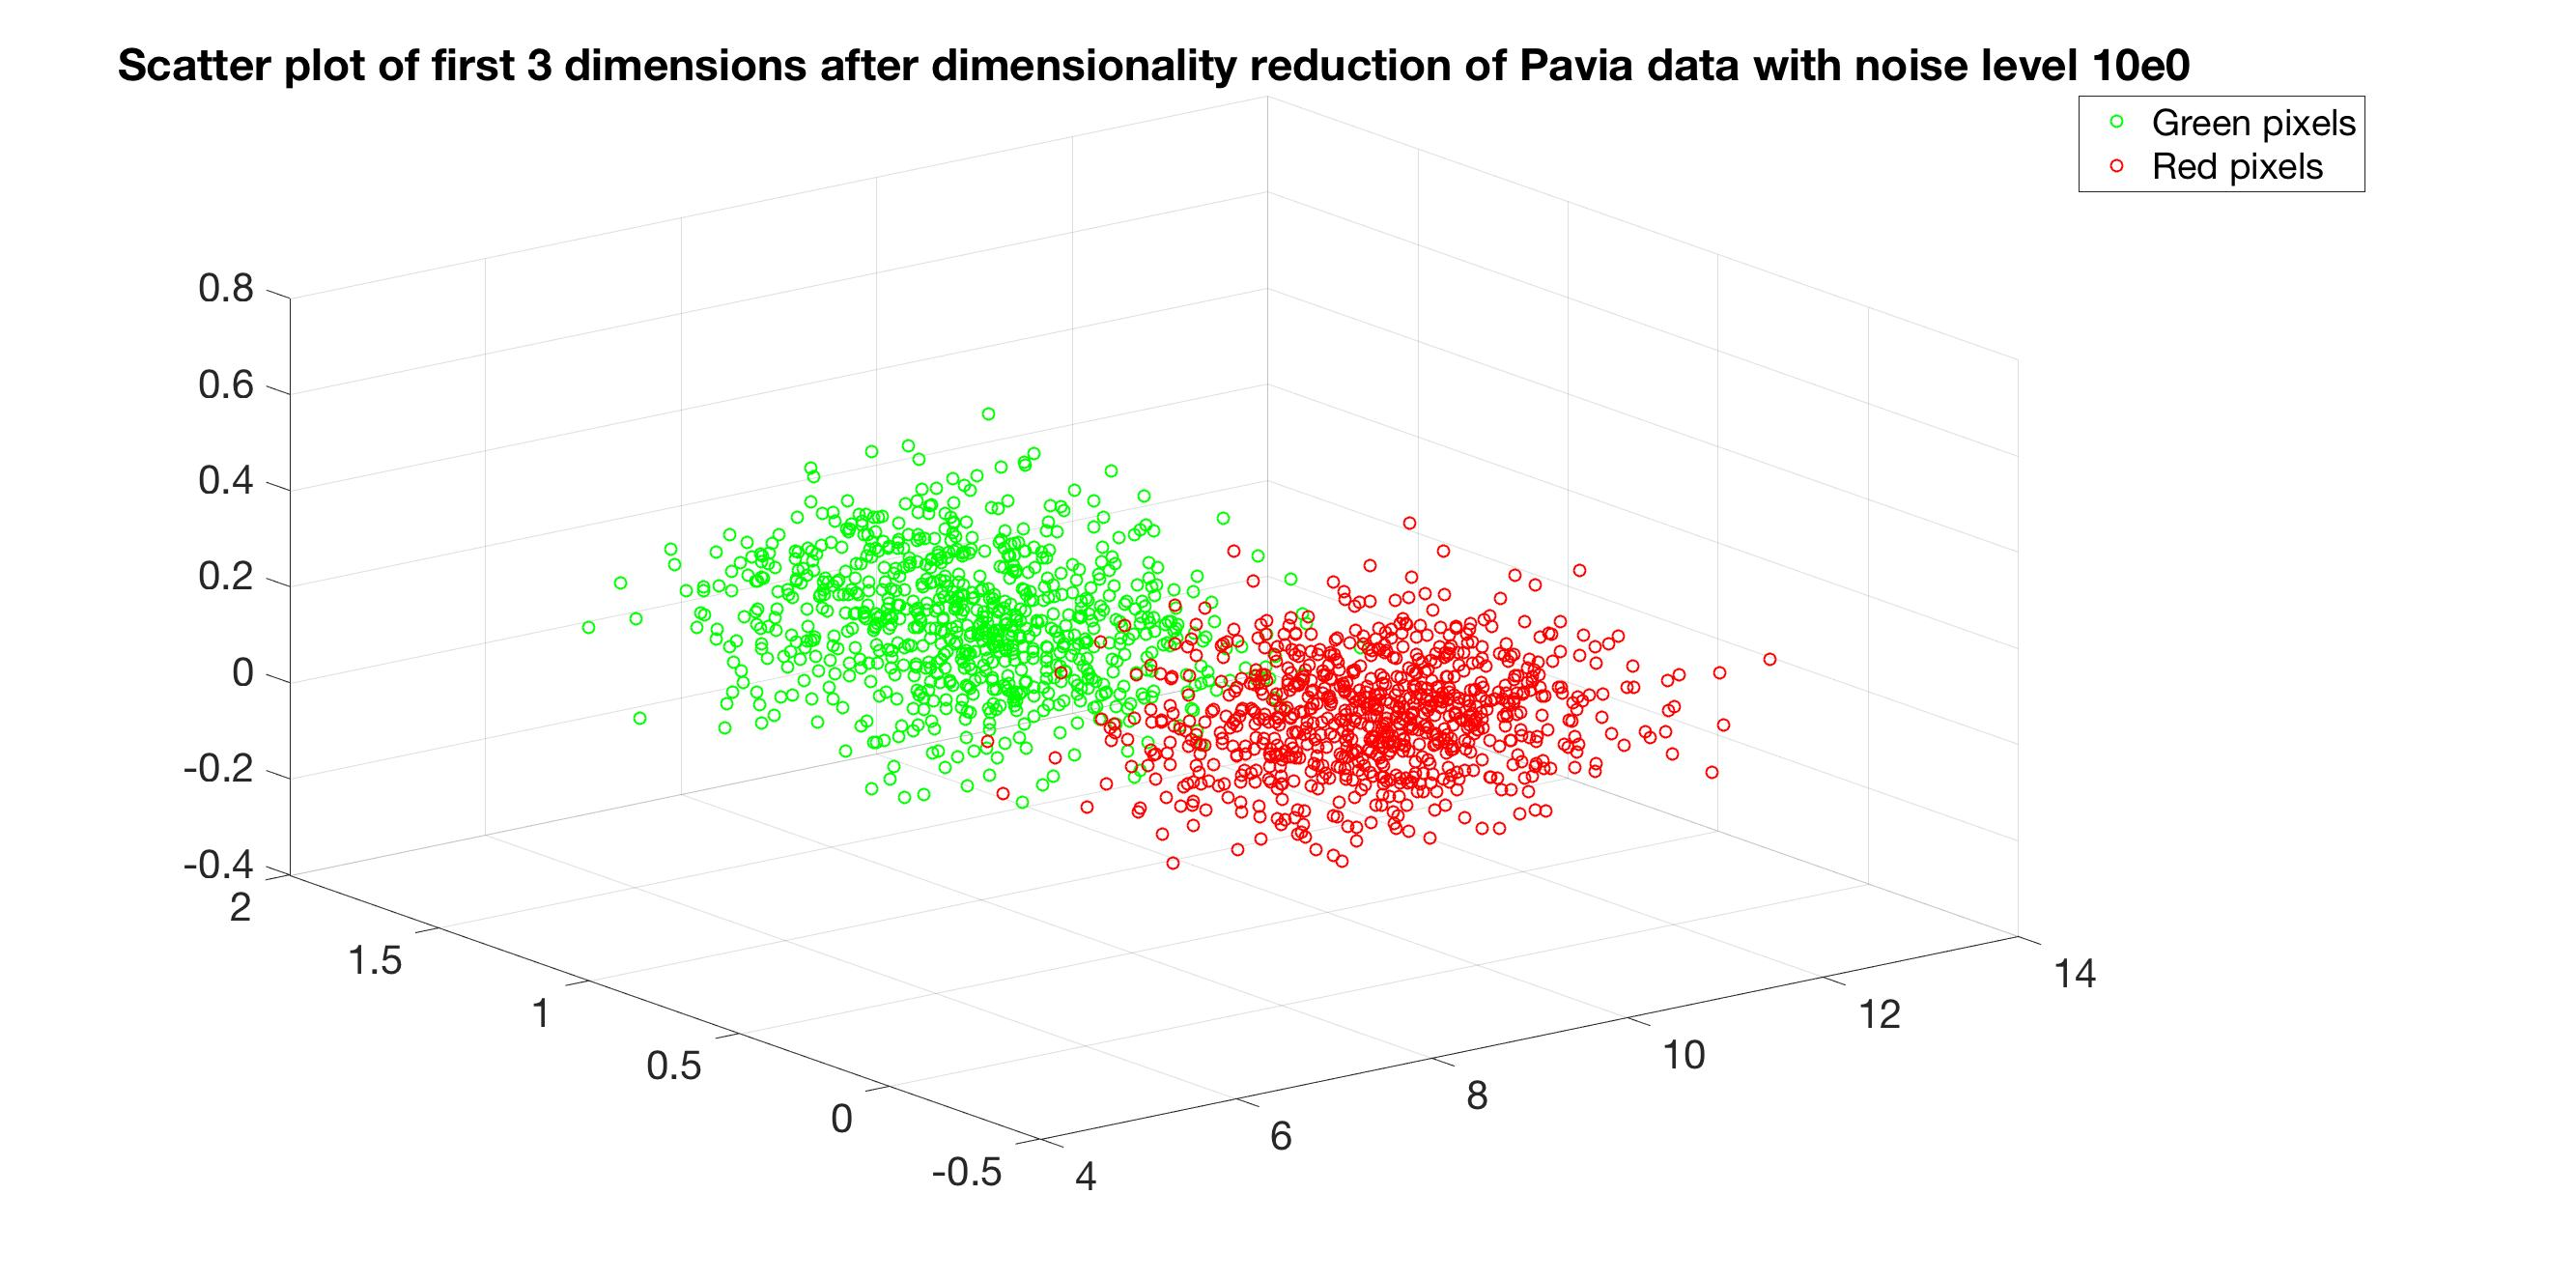
\includegraphics[width=.18\linewidth]{Noisescattermnf0.jpg}}}	
	\subfloat{{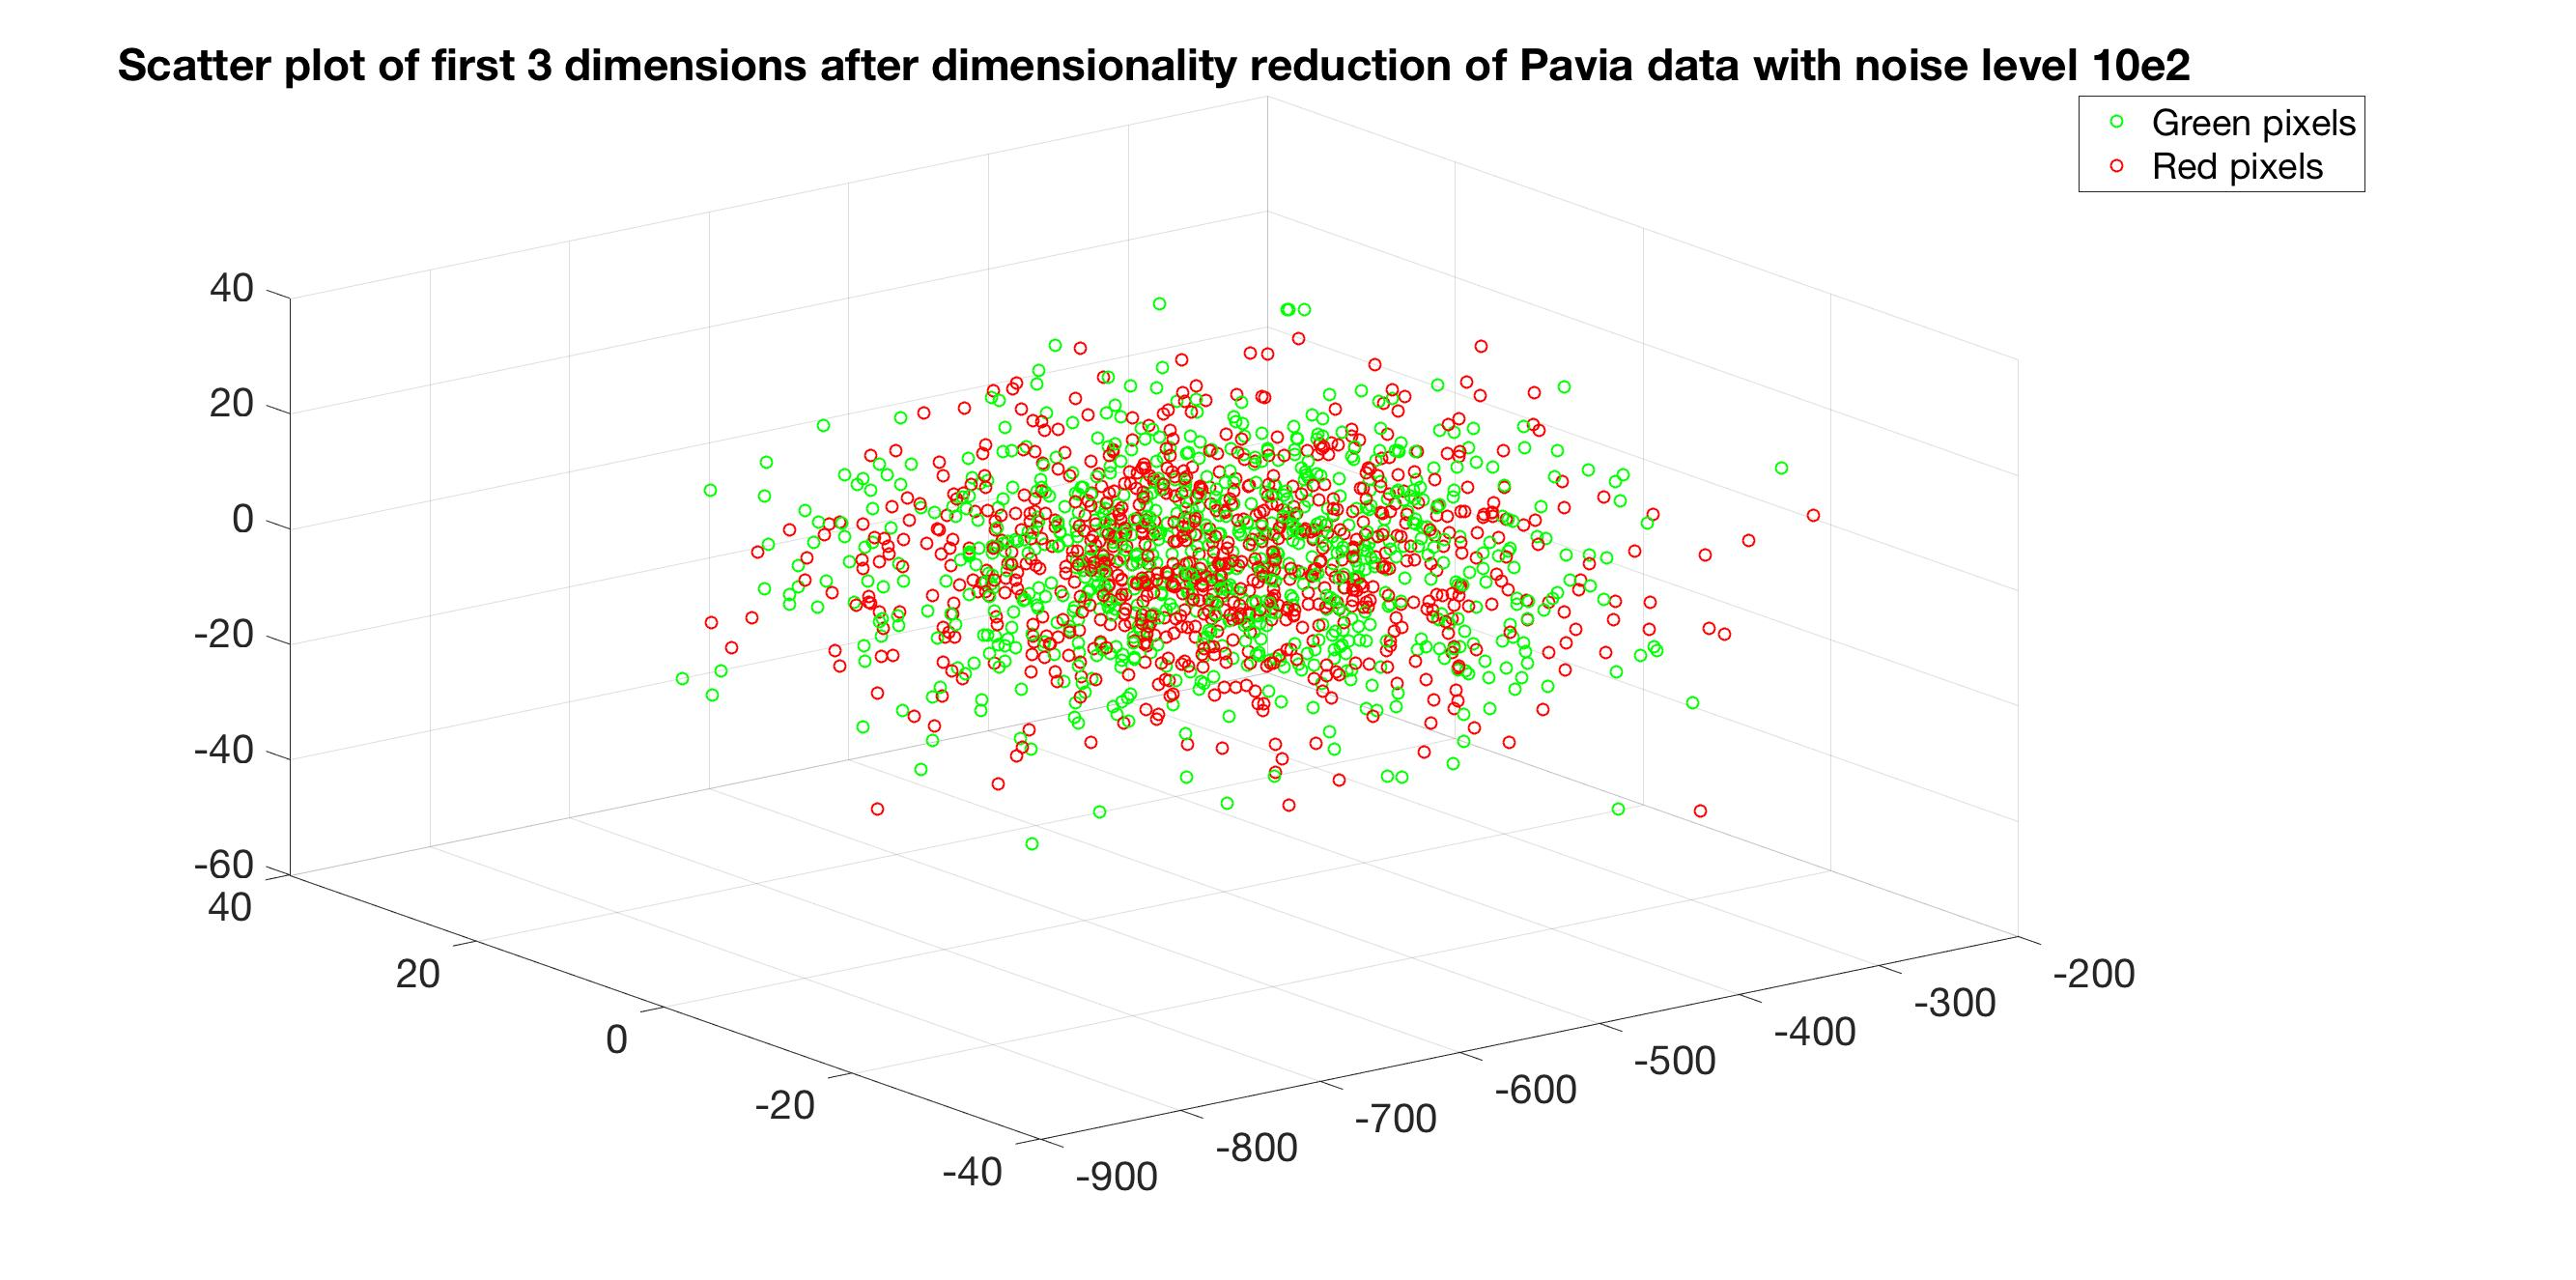
\includegraphics[width=.18\linewidth]{Noisescattermnf2.jpg}}}	
	\subfloat{{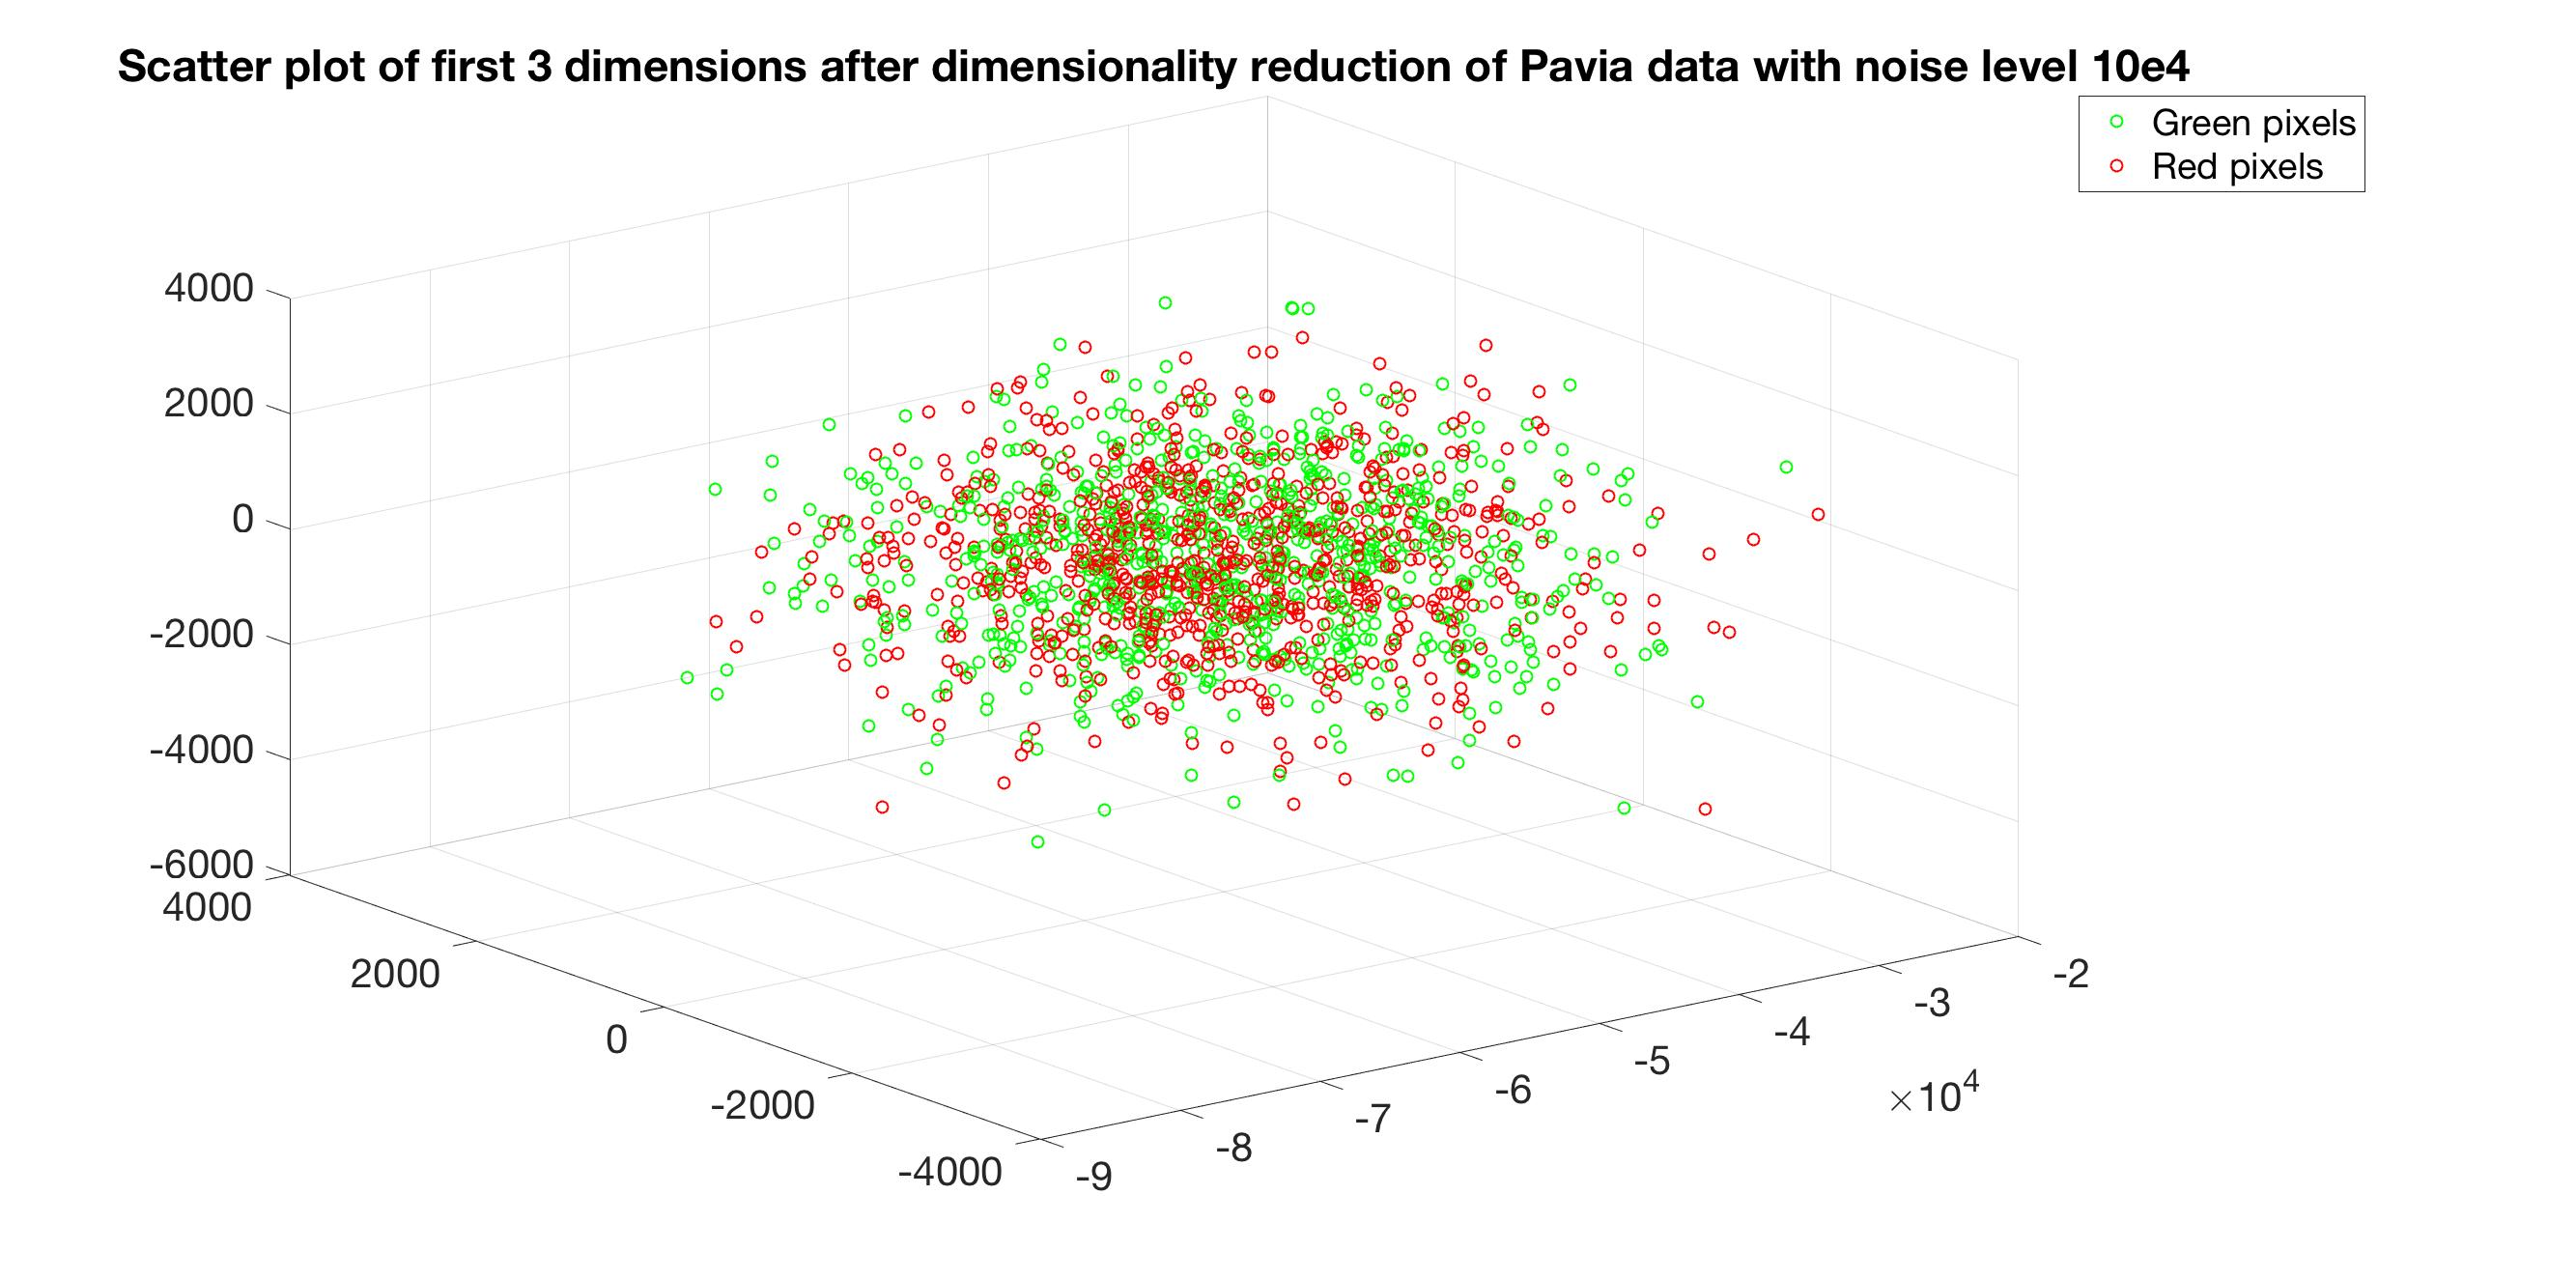
\includegraphics[width=.18\linewidth]{Noisescattermnf4.jpg}}}	
	\caption{Scatter plot of first 3 components after dimensionality using MNF with noise added to the fake Pavia image}
	\label{Paviamnfscatter}
\end{figure}

The  mean over all bands with noise added for the squeezed fake Pavia image are shown below in figure \ref{sqPaviamean}; the corresponding mean over all bands of the corresponding dimensionality reduction results are shown in figure \ref{sqPaviamnfmean}; and the corresponding scatter plot of first 3 components after dimensionality using MNF is shown in figure \ref{sqPaviamnfscatter}.
\begin{figure}[H]
	\centering
	\subfloat{{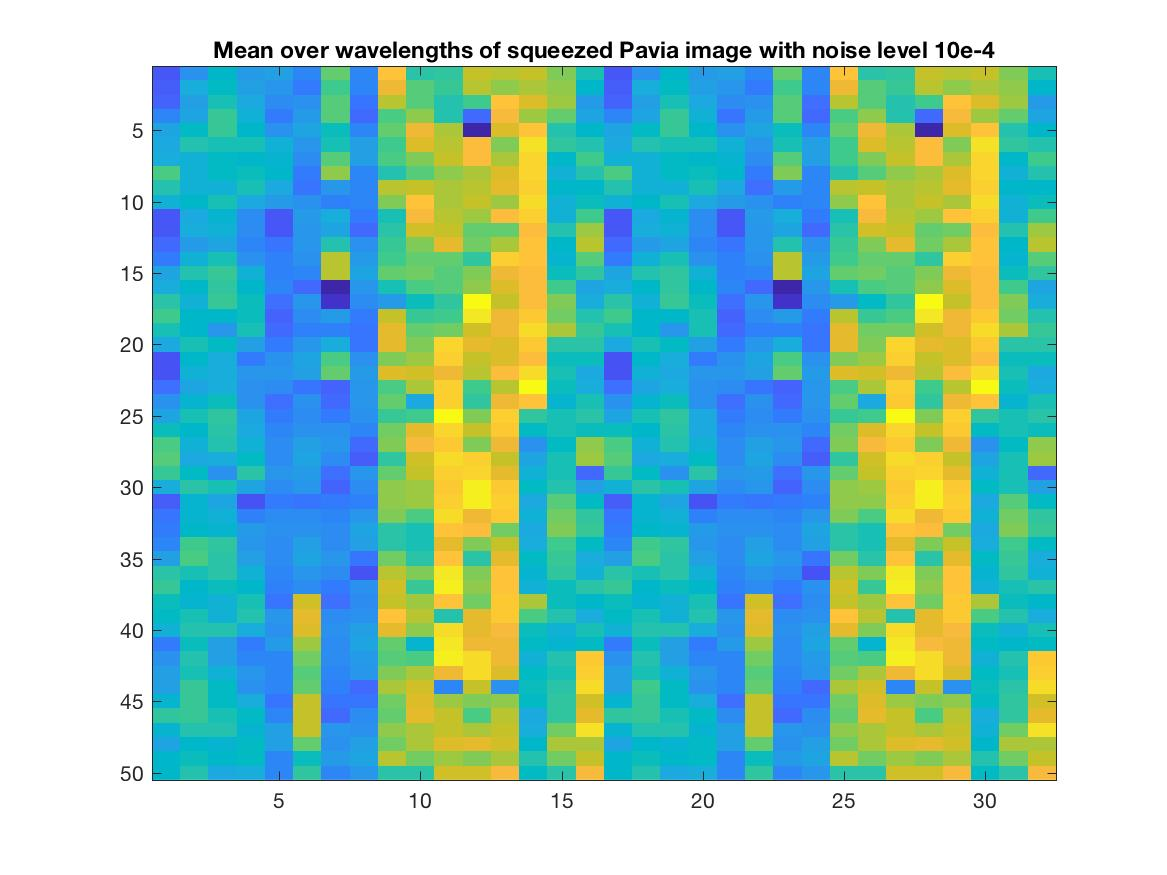
\includegraphics[width=.18\linewidth]{meansqueezed-4.jpg}}}
	\subfloat{{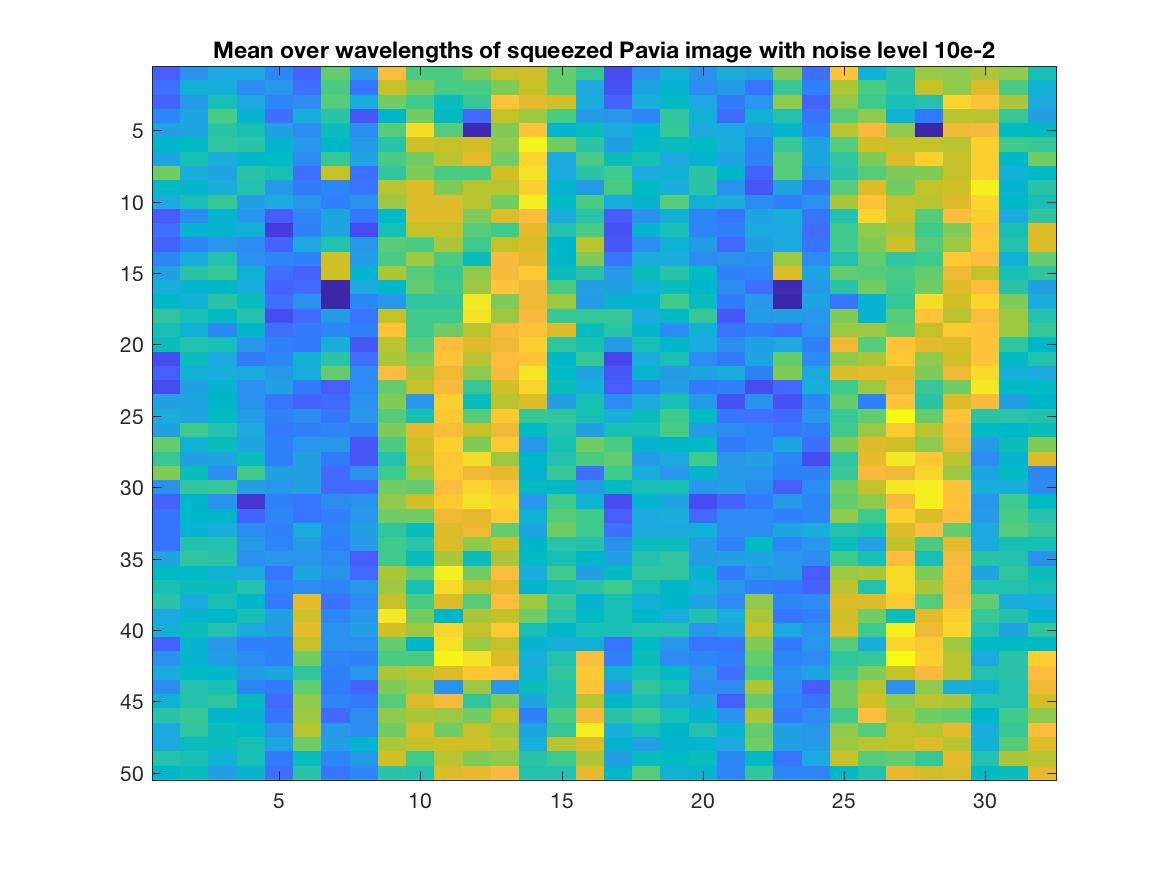
\includegraphics[width=.18\linewidth]{meansqueezed-2.jpg}}}	
	\subfloat{{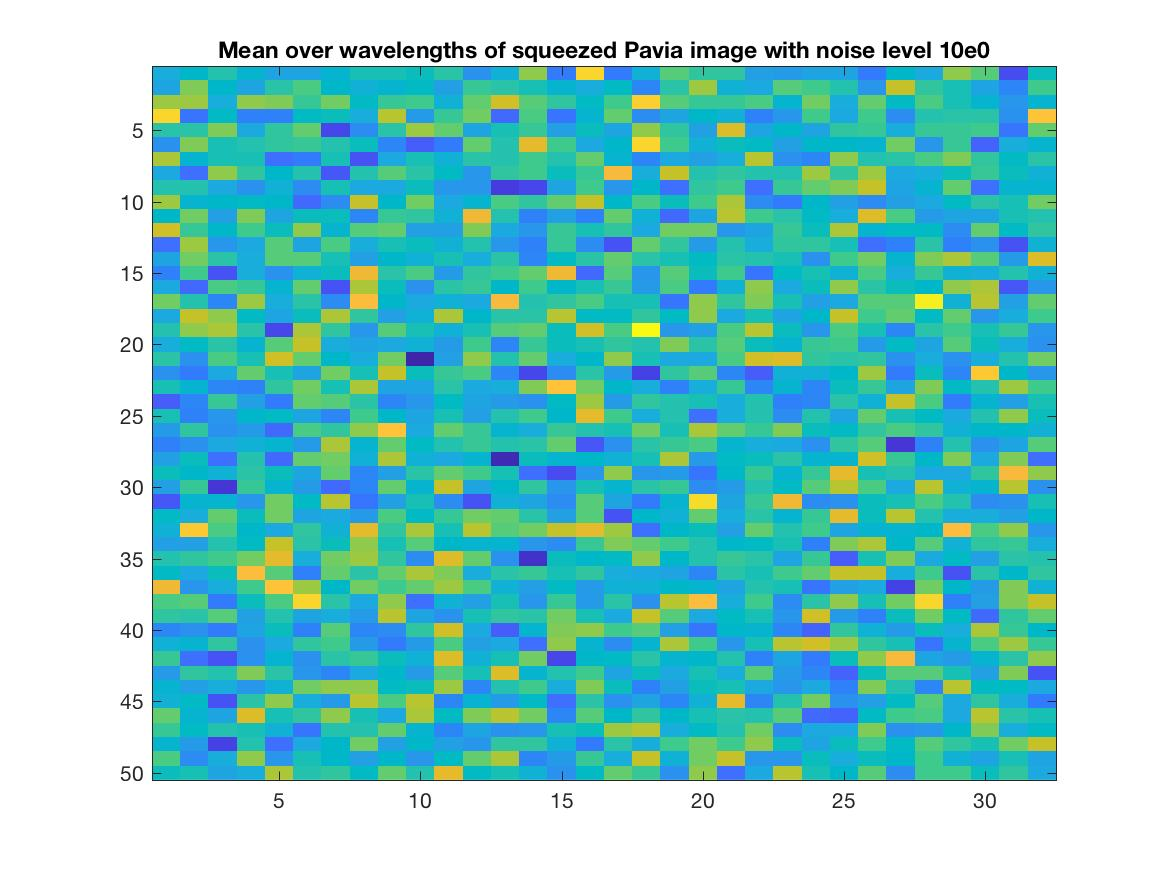
\includegraphics[width=.18\linewidth]{meansqueezed0.jpg}}}	
	\subfloat{{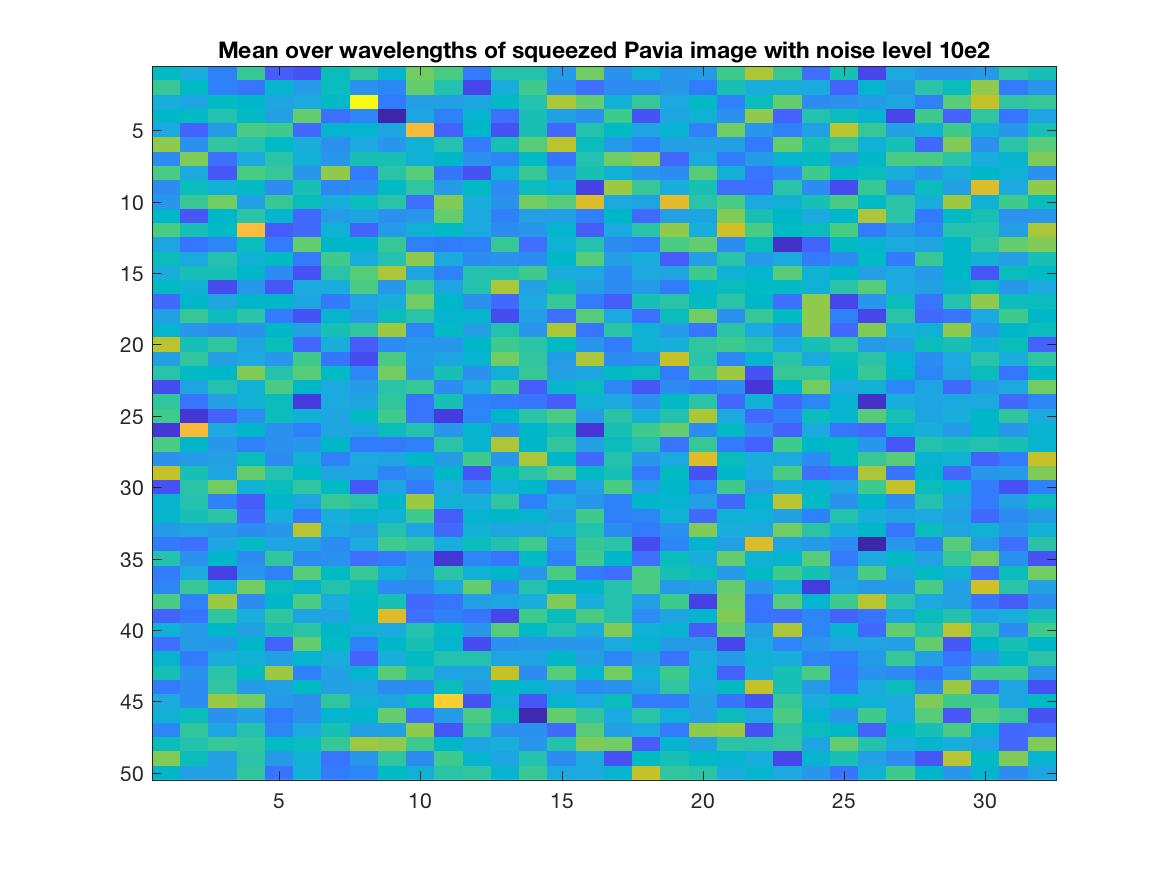
\includegraphics[width=.18\linewidth]{meansqueezed2.jpg}}}	
	\subfloat{{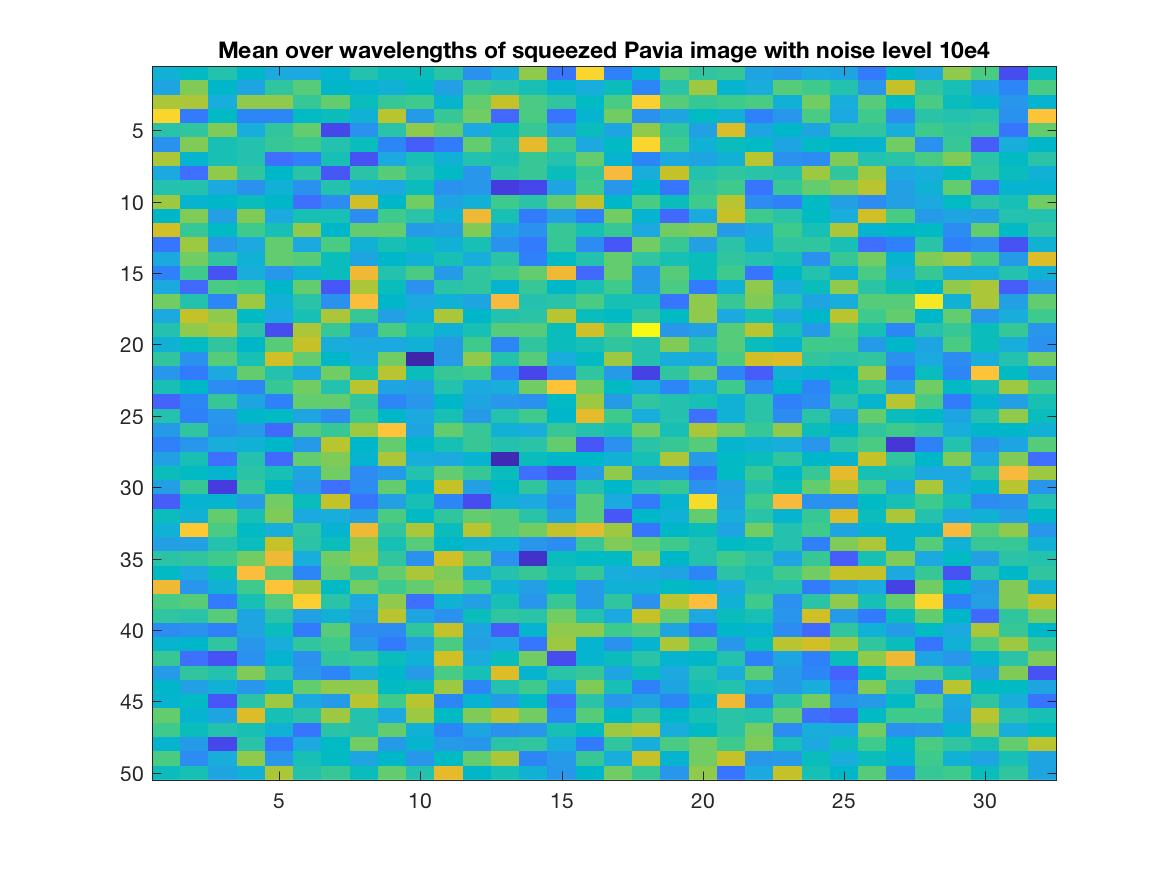
\includegraphics[width=.18\linewidth]{meansqueezed4.jpg}}}	
	\caption{Mean over all bands after adding noise for squeezed fake Pavia image}
	\label{sqPaviamean}
\end{figure}

\begin{figure}[H]
	\centering
	\subfloat{{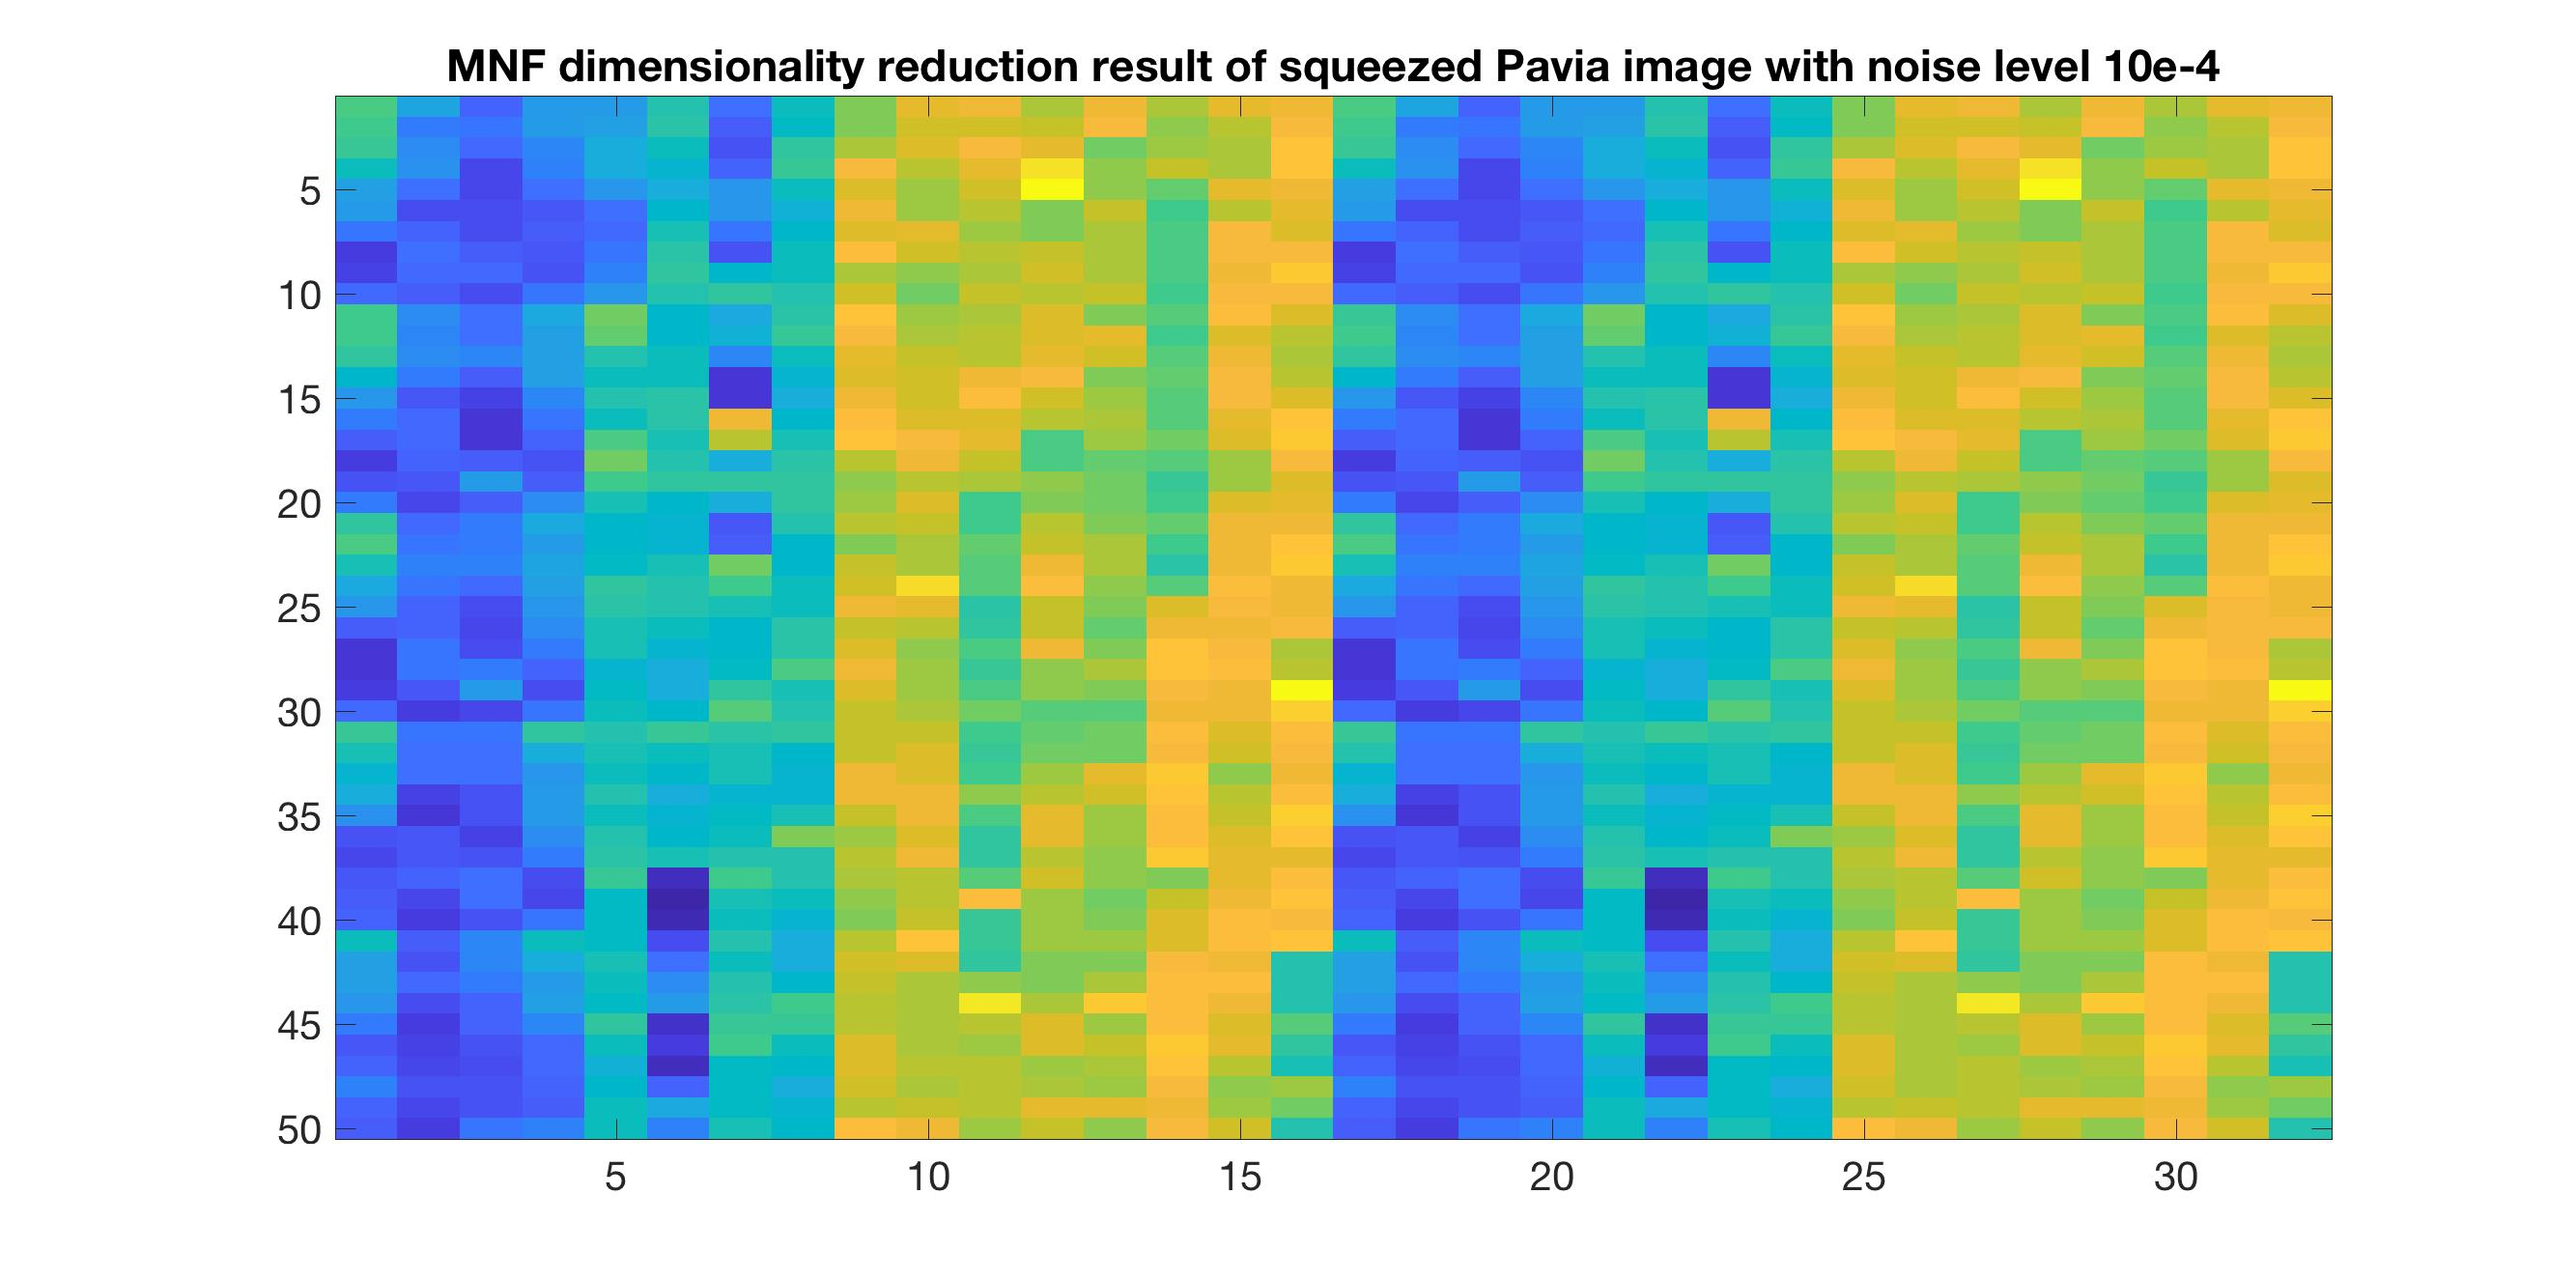
\includegraphics[width=.18\linewidth]{mnfsqueezed-4.jpg}}}
	\subfloat{{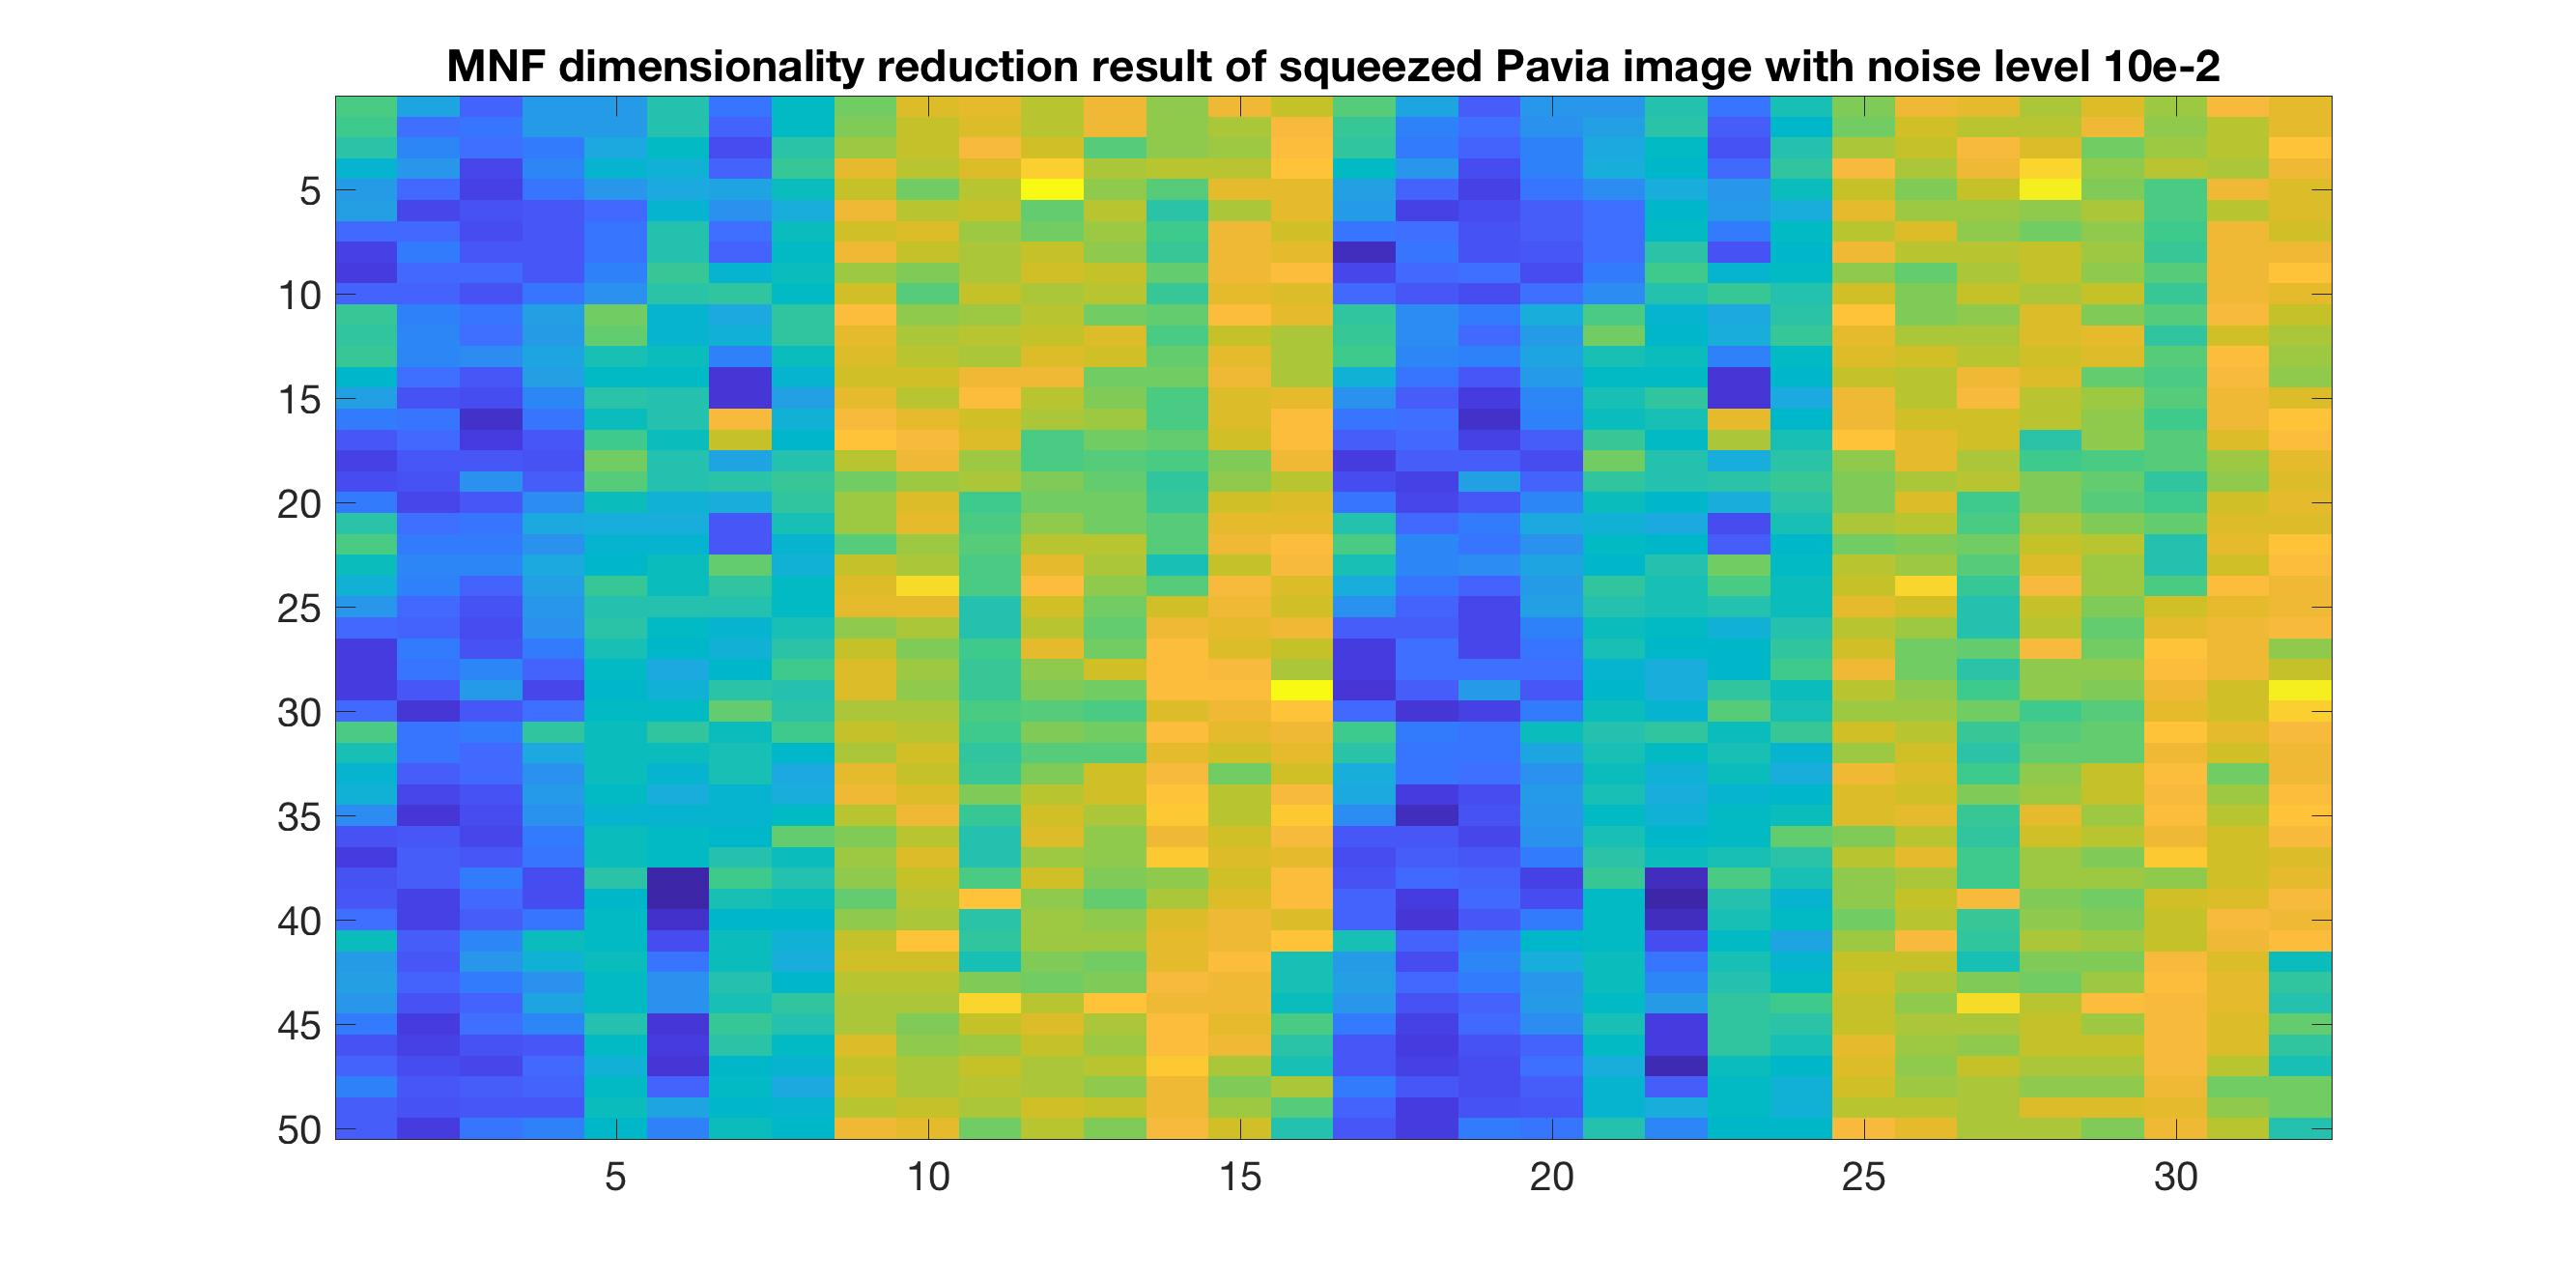
\includegraphics[width=.18\linewidth]{mnfsqueezed-2.jpg}}}	
	\subfloat{{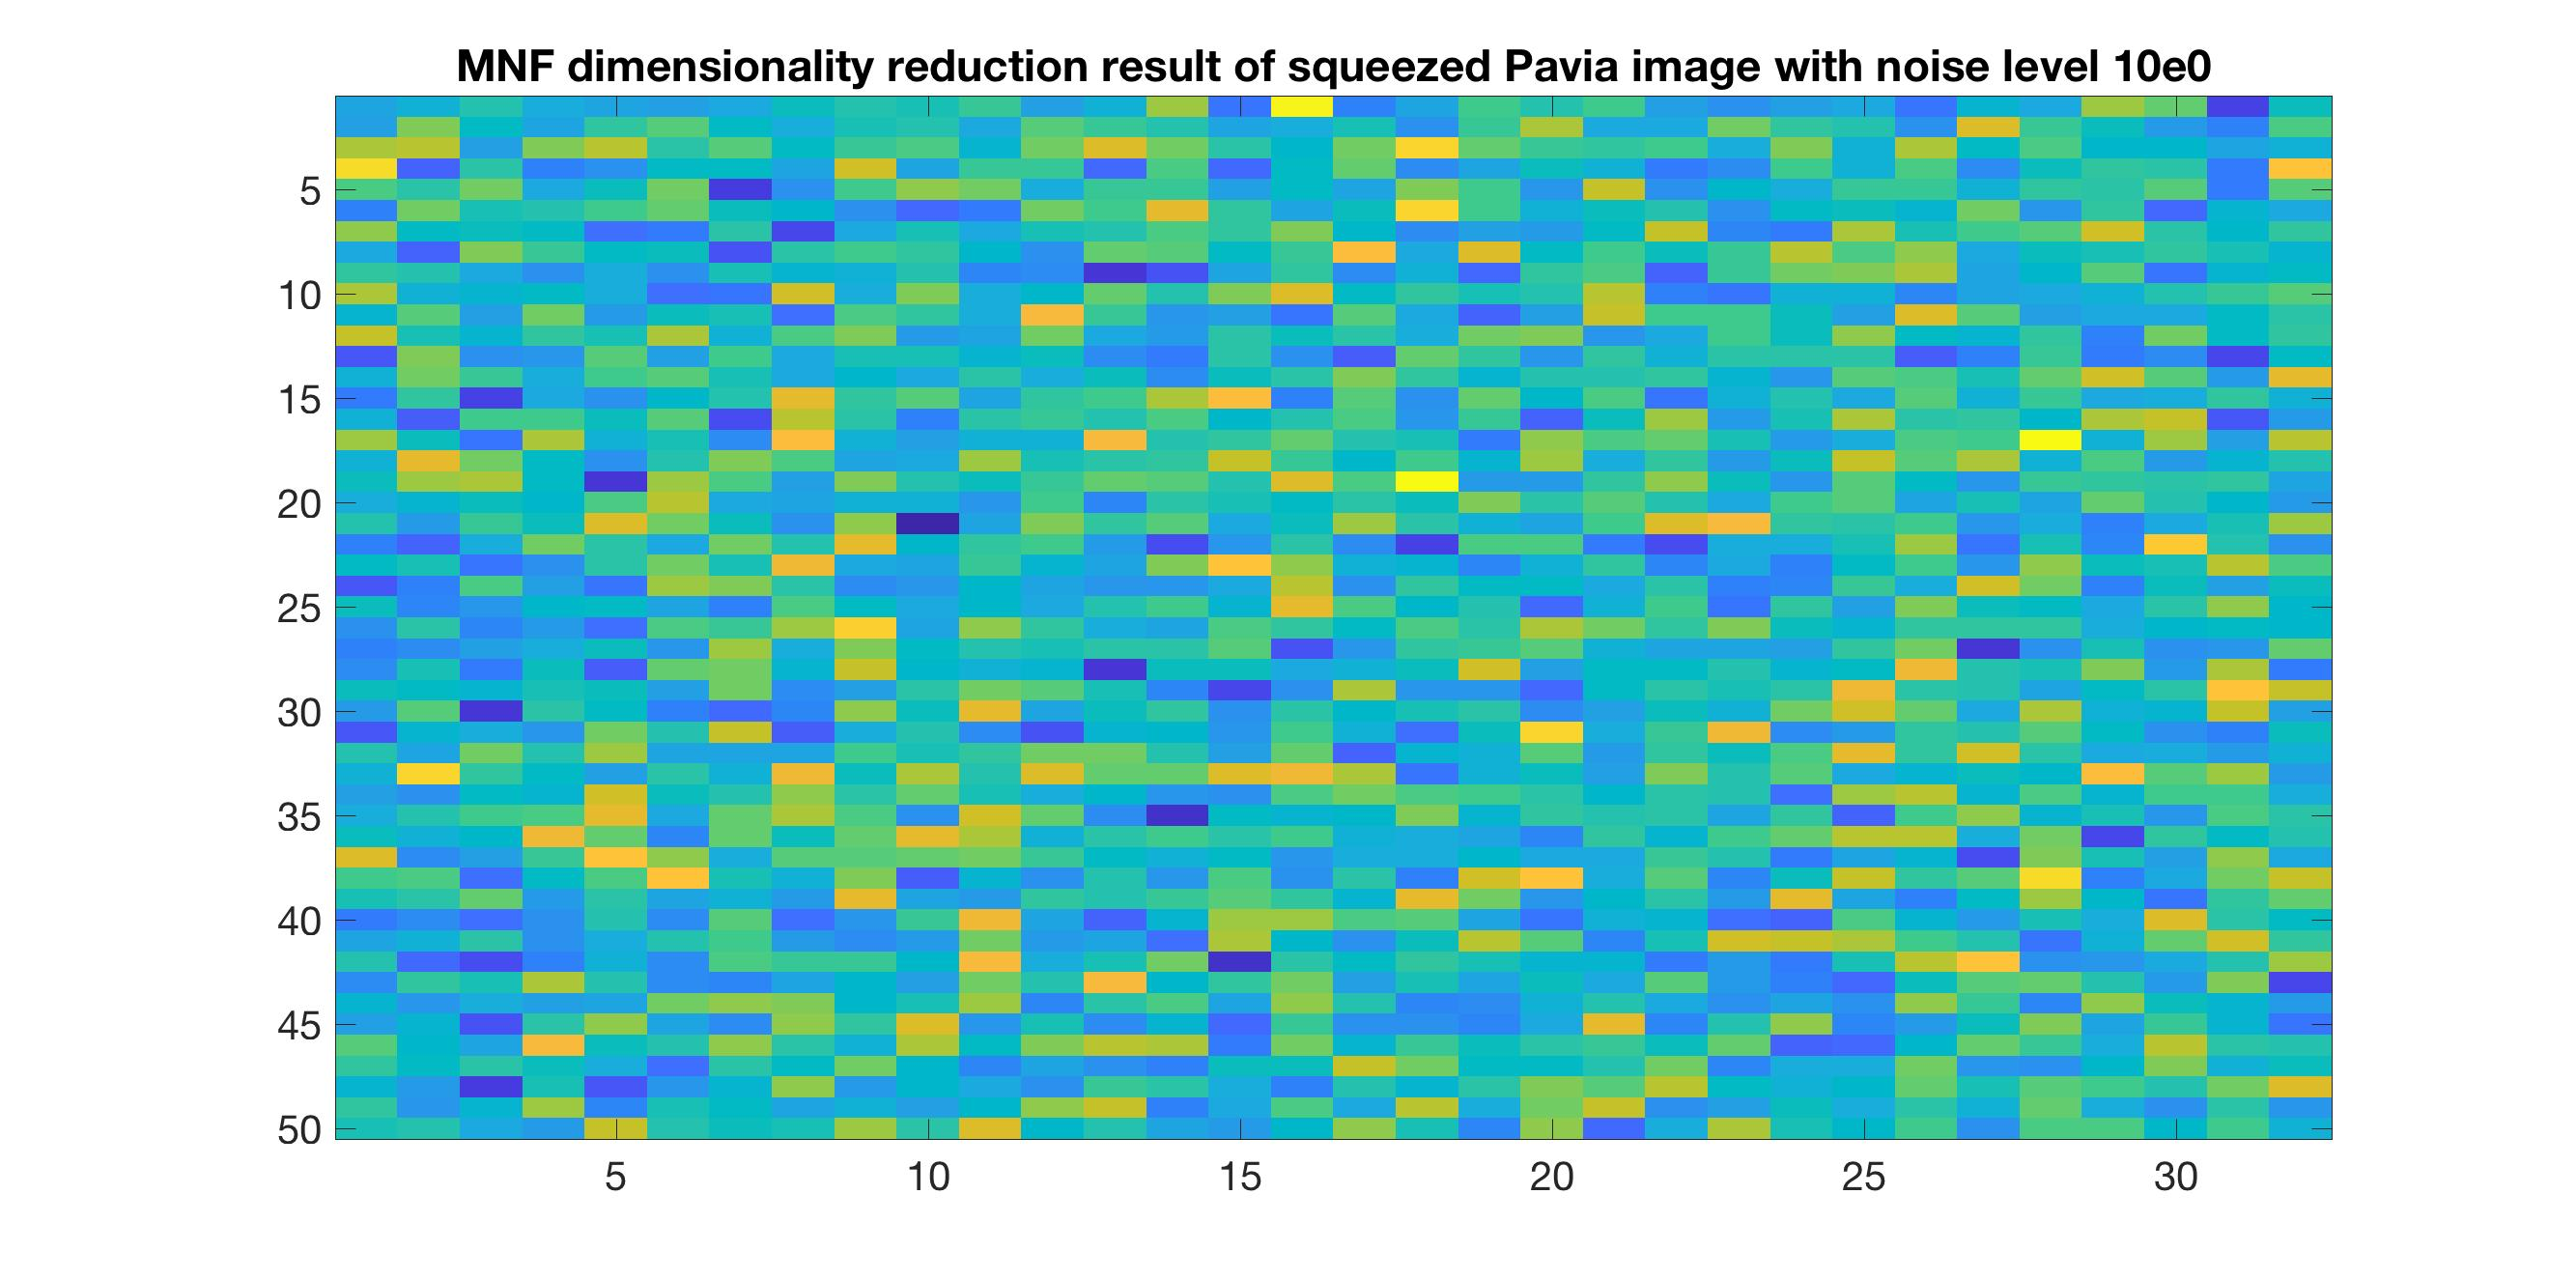
\includegraphics[width=.18\linewidth]{mnfsqueezed0.jpg}}}	
	\subfloat{{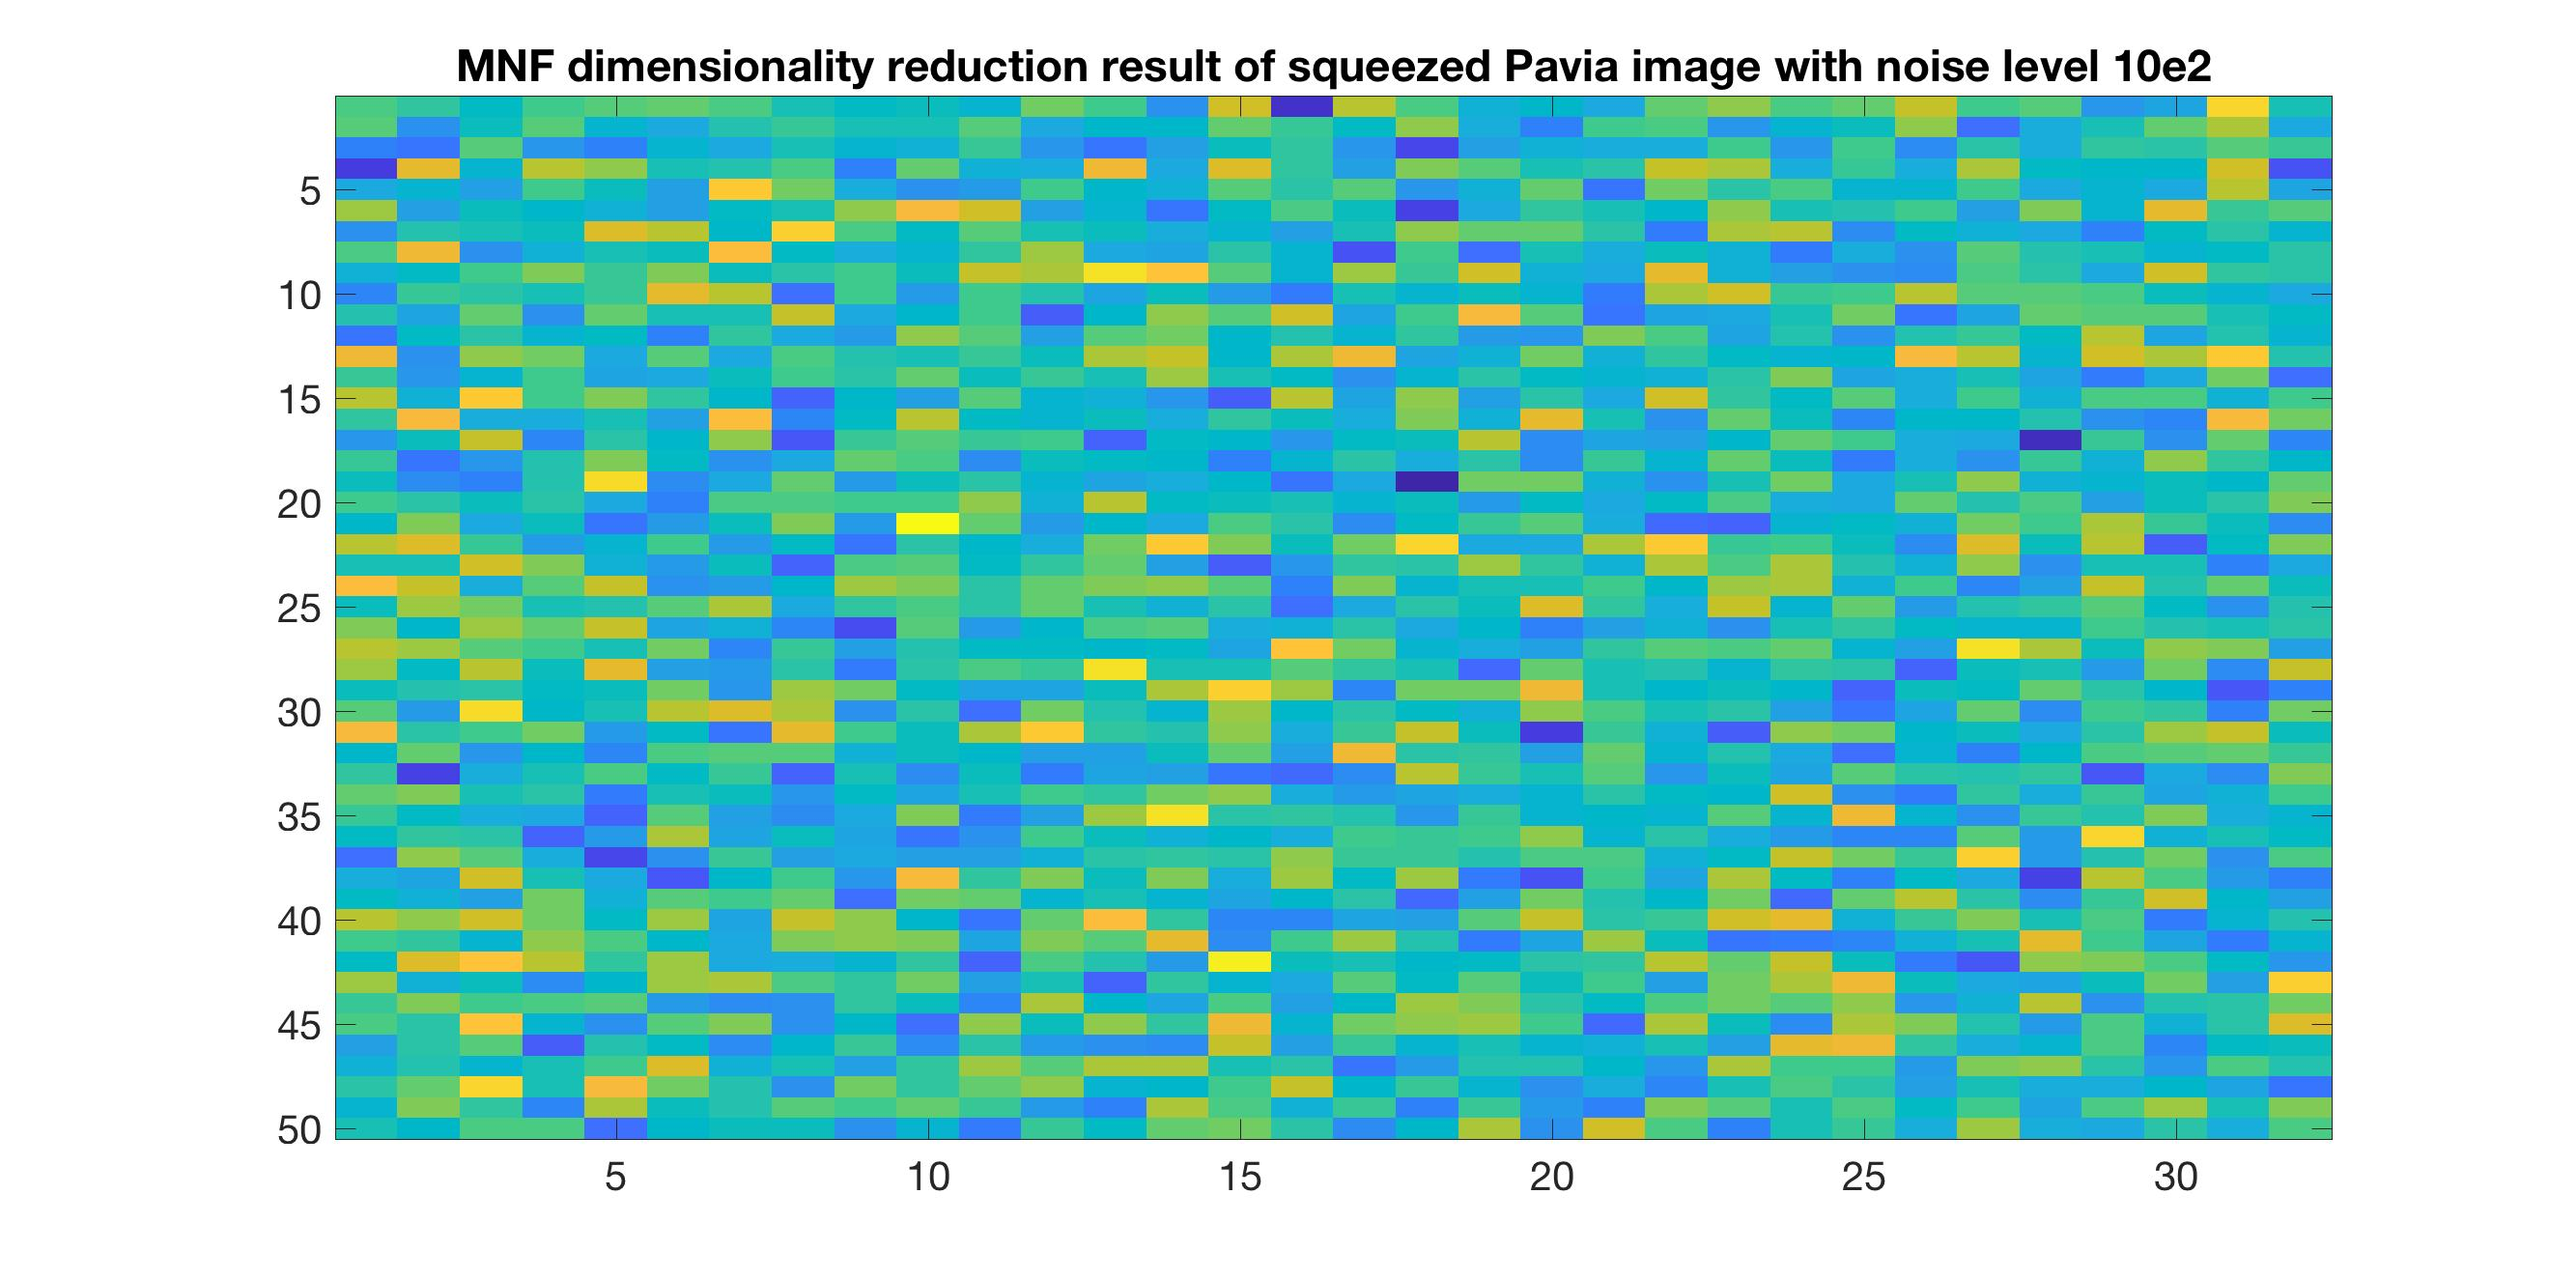
\includegraphics[width=.18\linewidth]{mnfsqueezed2.jpg}}}	
	\subfloat{{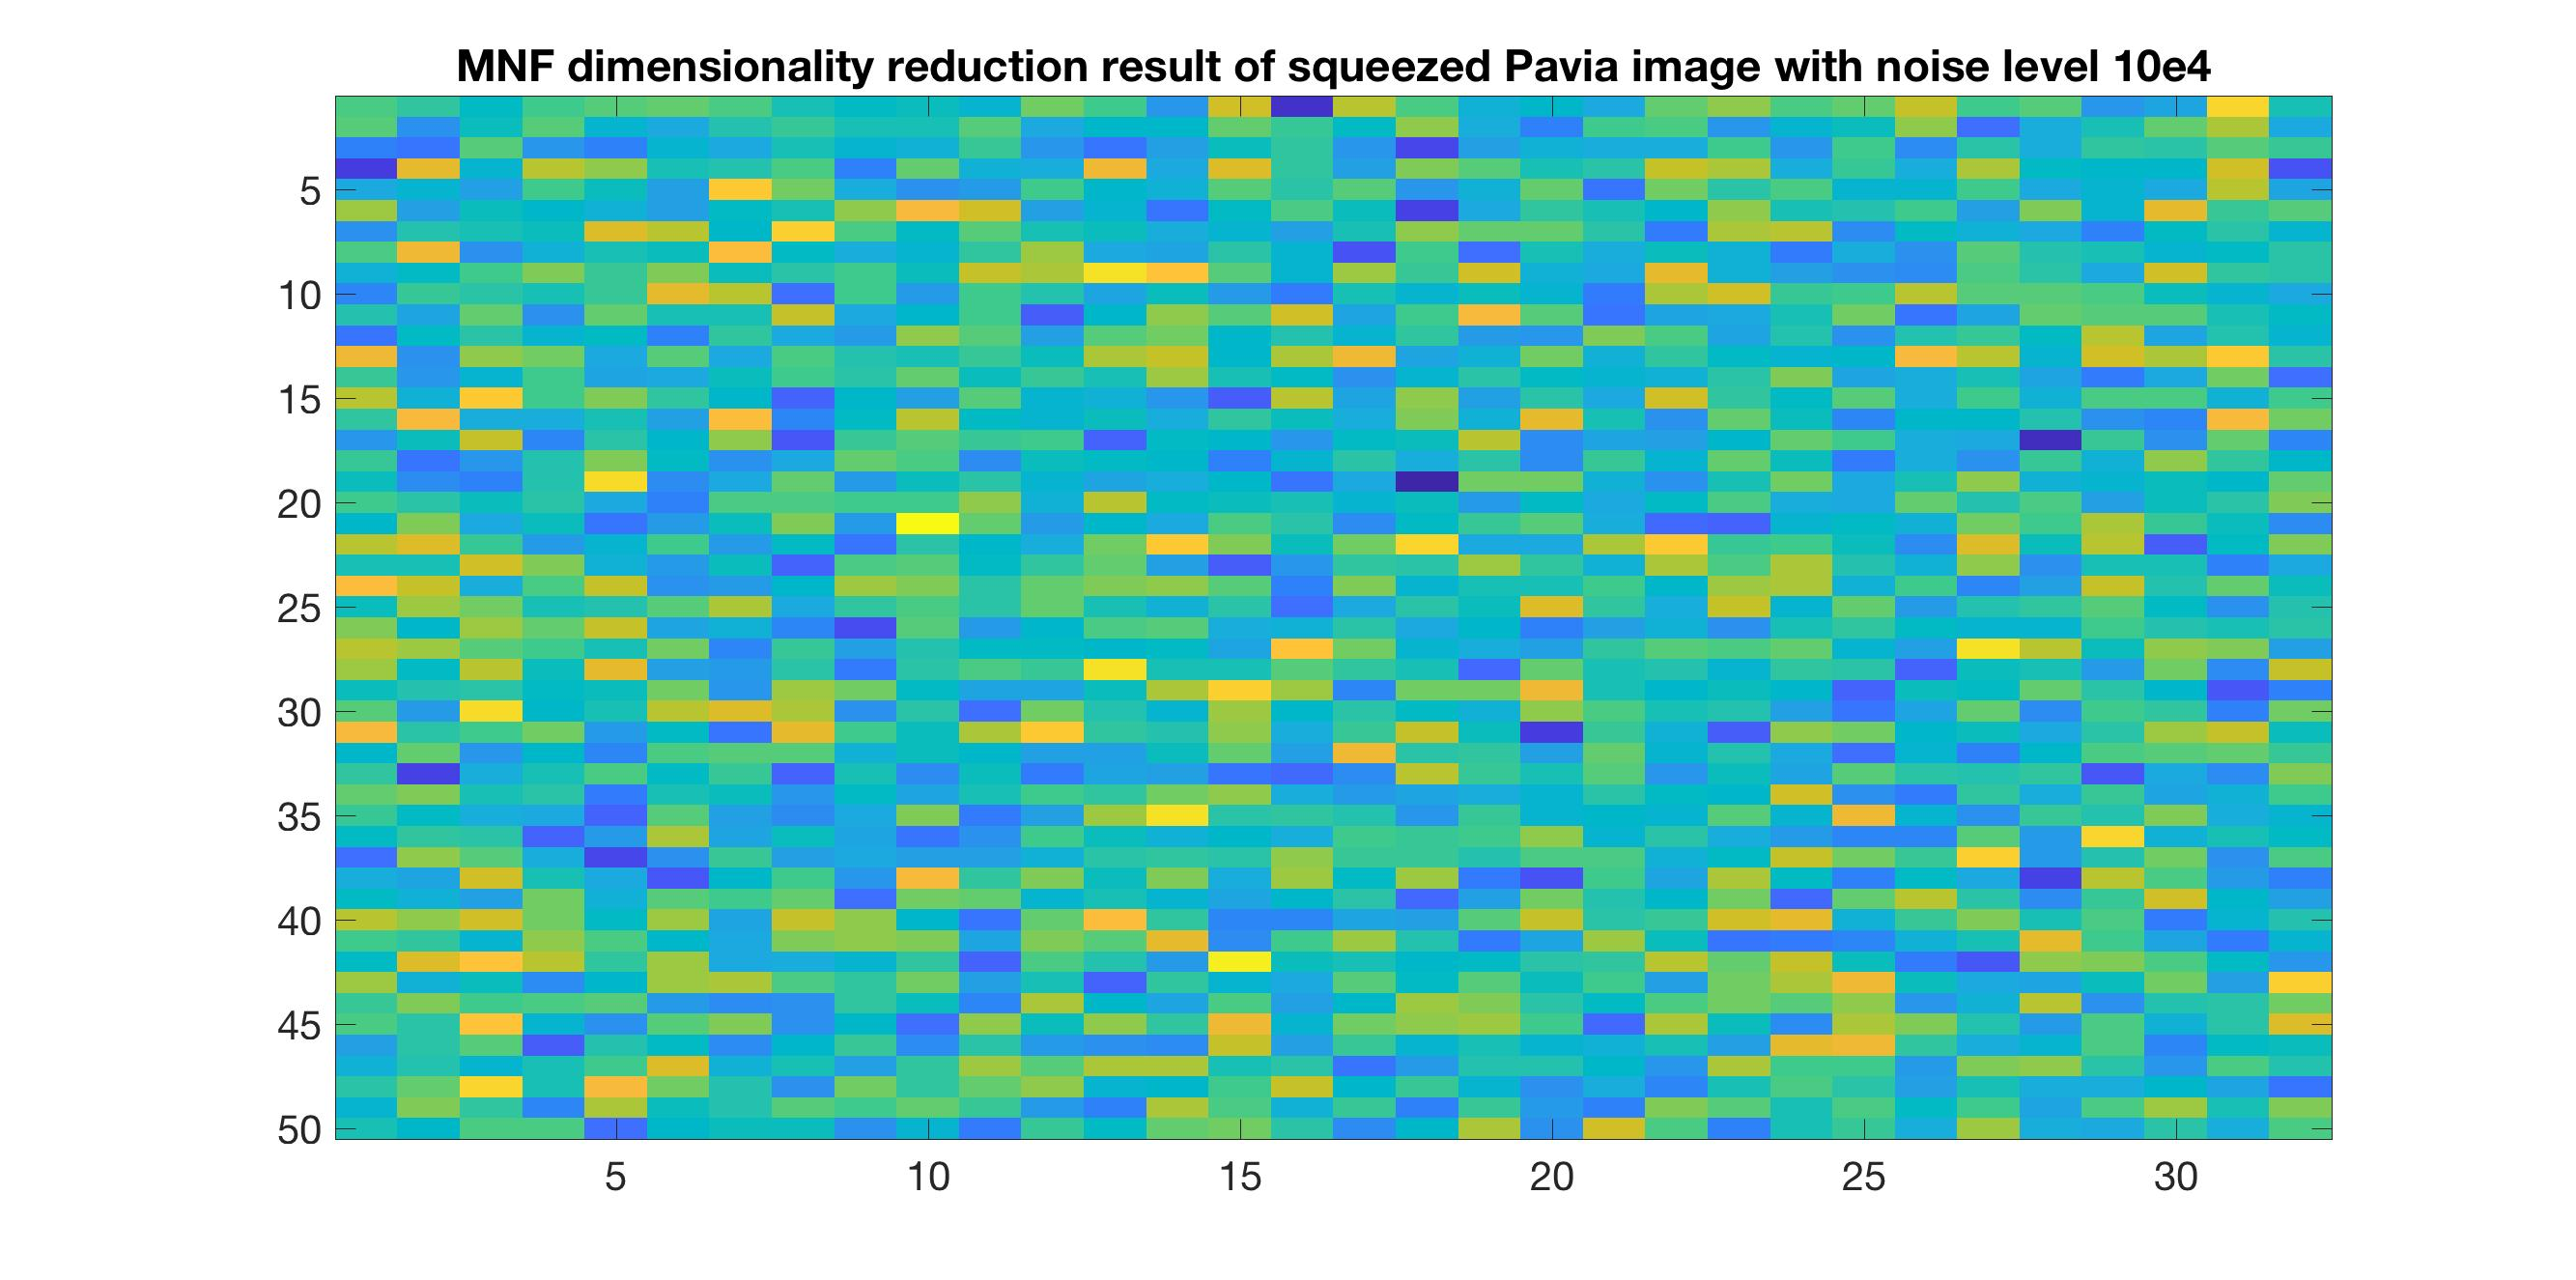
\includegraphics[width=.18\linewidth]{mnfsqueezed4.jpg}}}	
	\caption{Mean over all bands after MNF dimensionality reduction with noise added  to the squeezed fake Pavia image}
	\label{sqPaviamnfmean}
\end{figure}

\begin{figure}[H]
	\centering
	\subfloat{{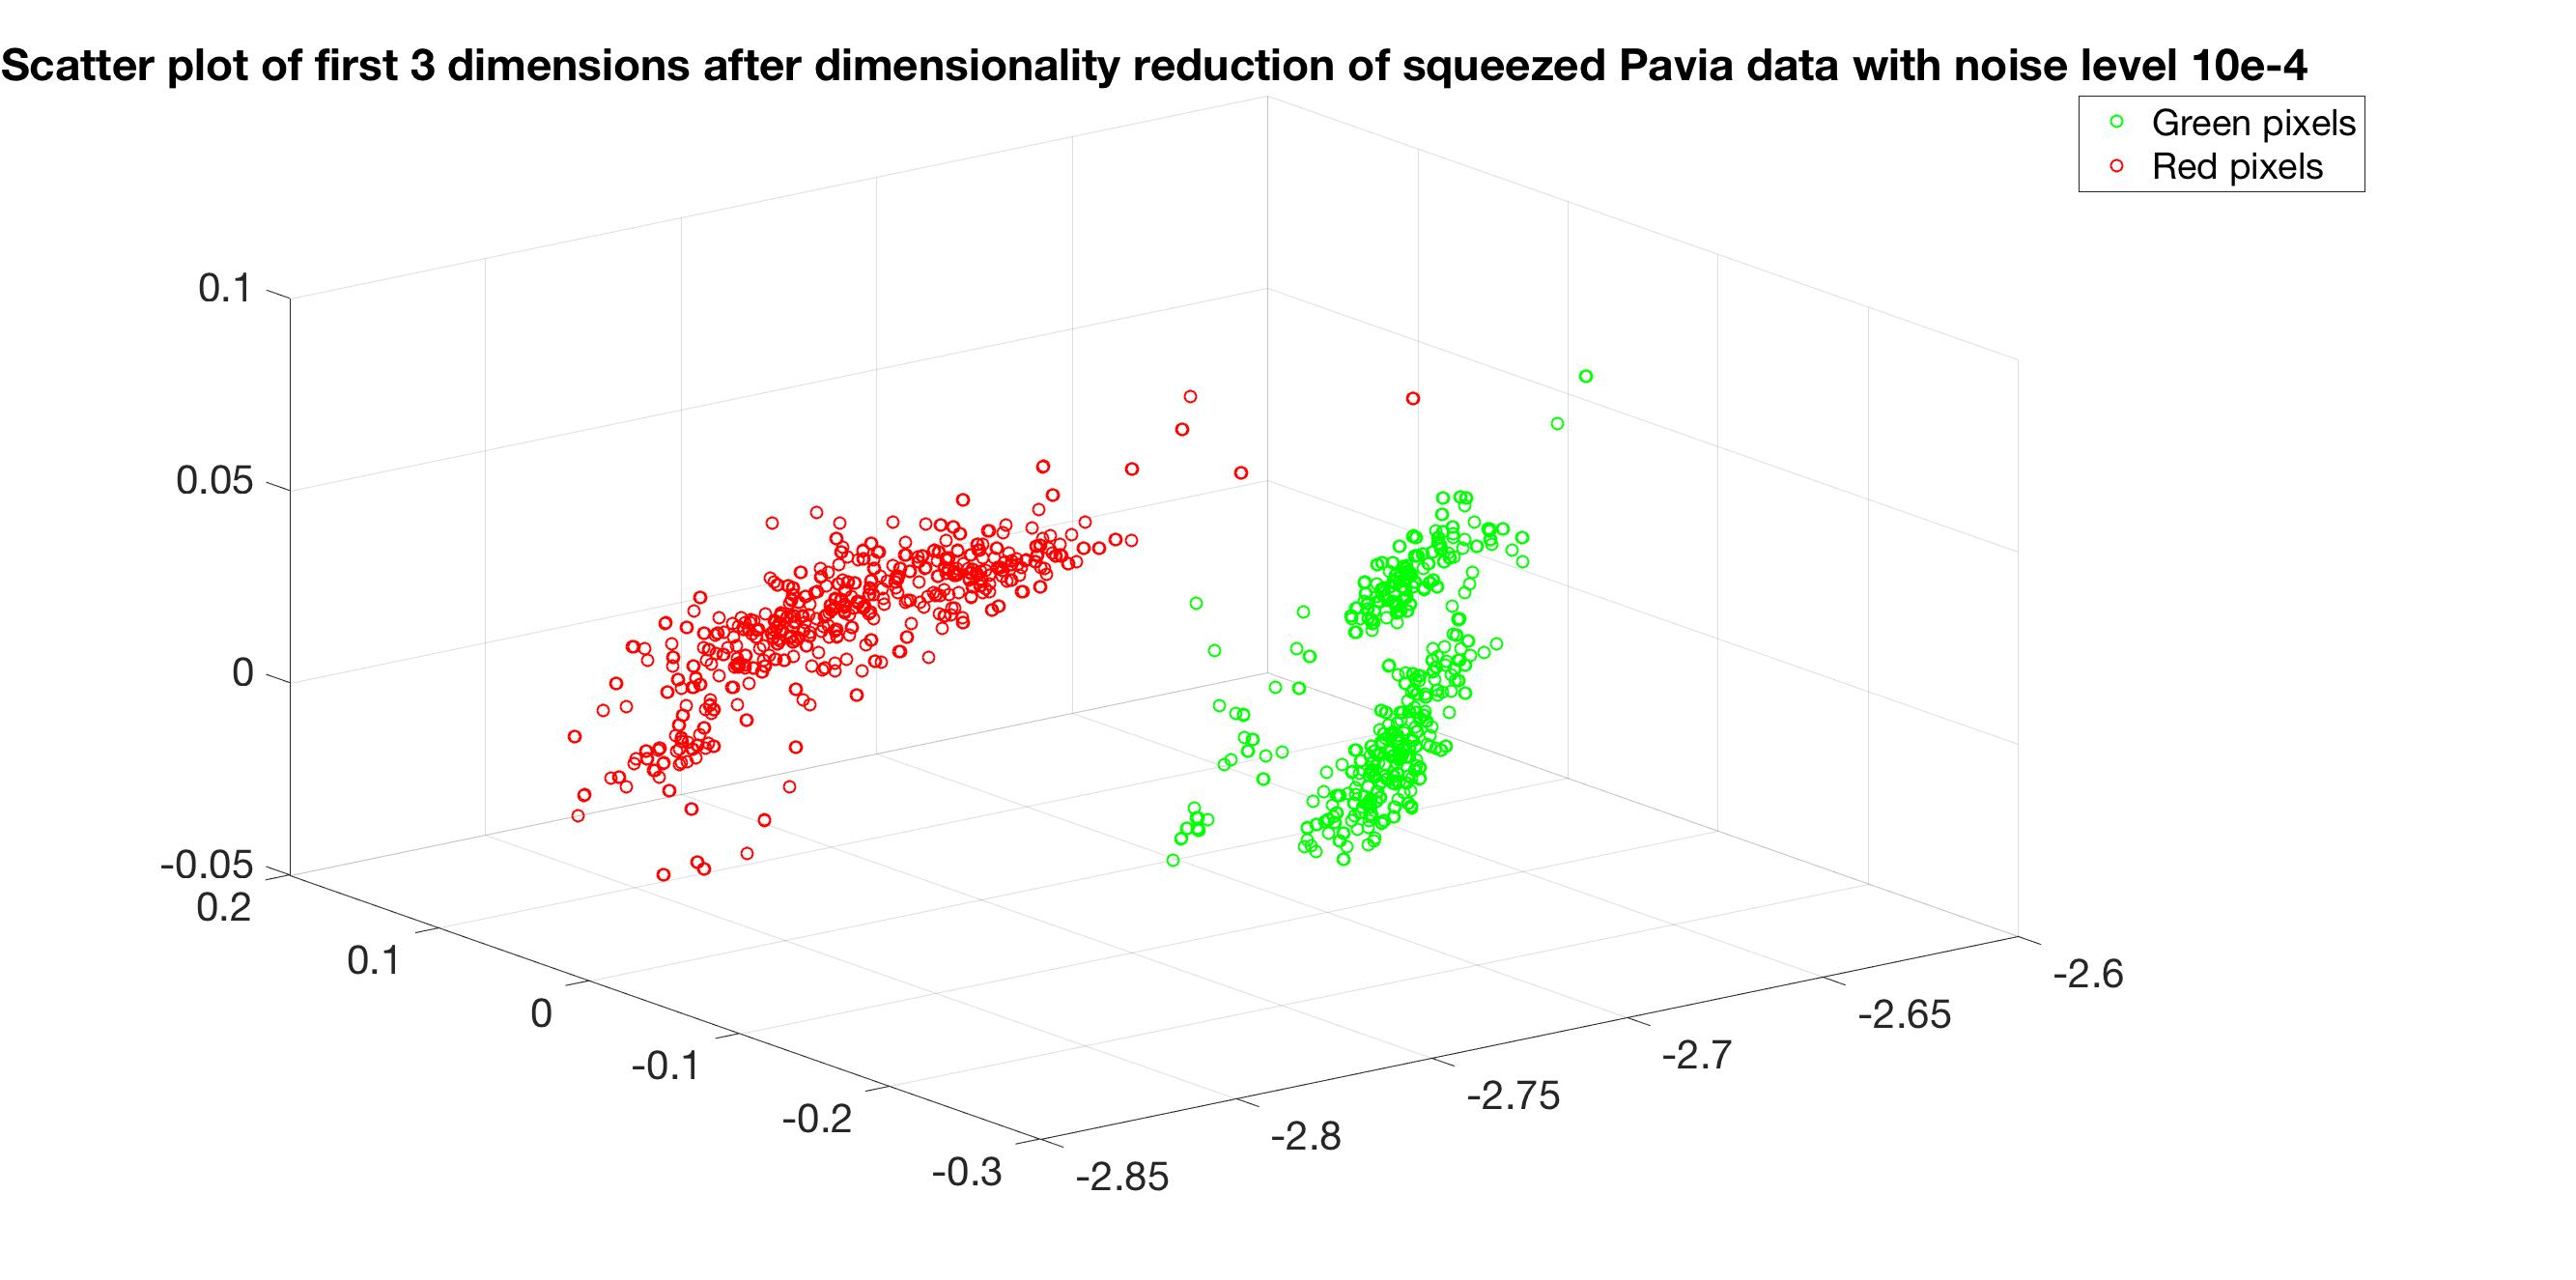
\includegraphics[width=.18\linewidth]{Noisescattermnfsqueezed-4.jpg}}}
	\subfloat{{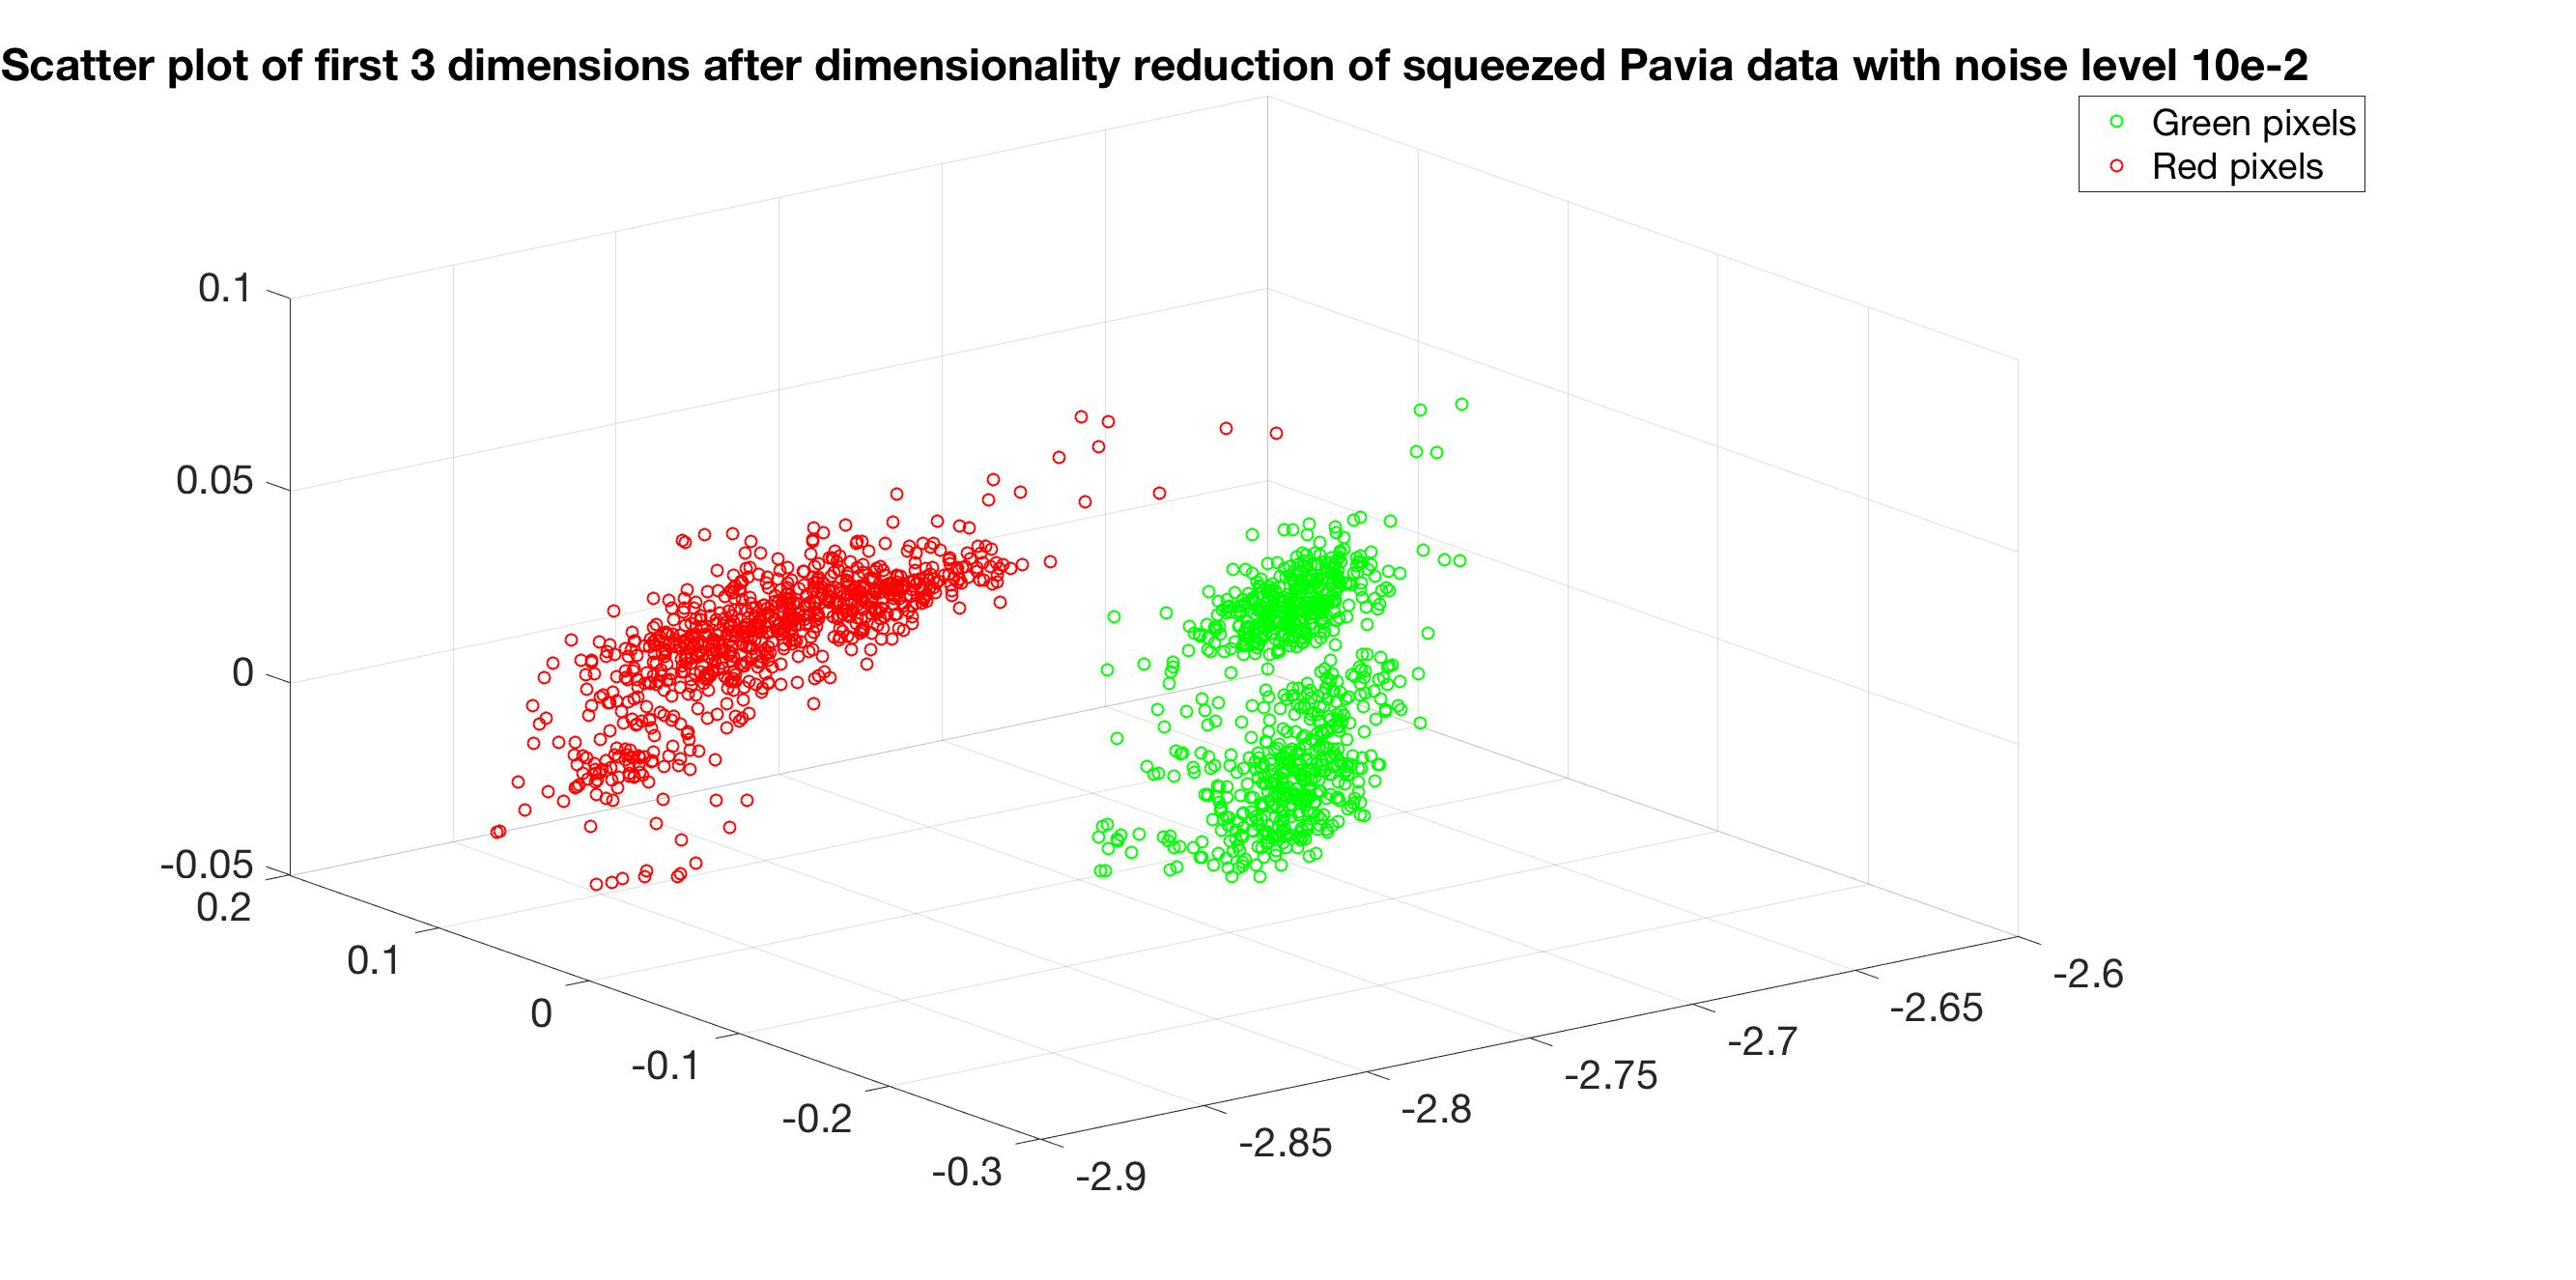
\includegraphics[width=.18\linewidth]{Noisescattermnfsqueezed-2.jpg}}}	
	\subfloat{{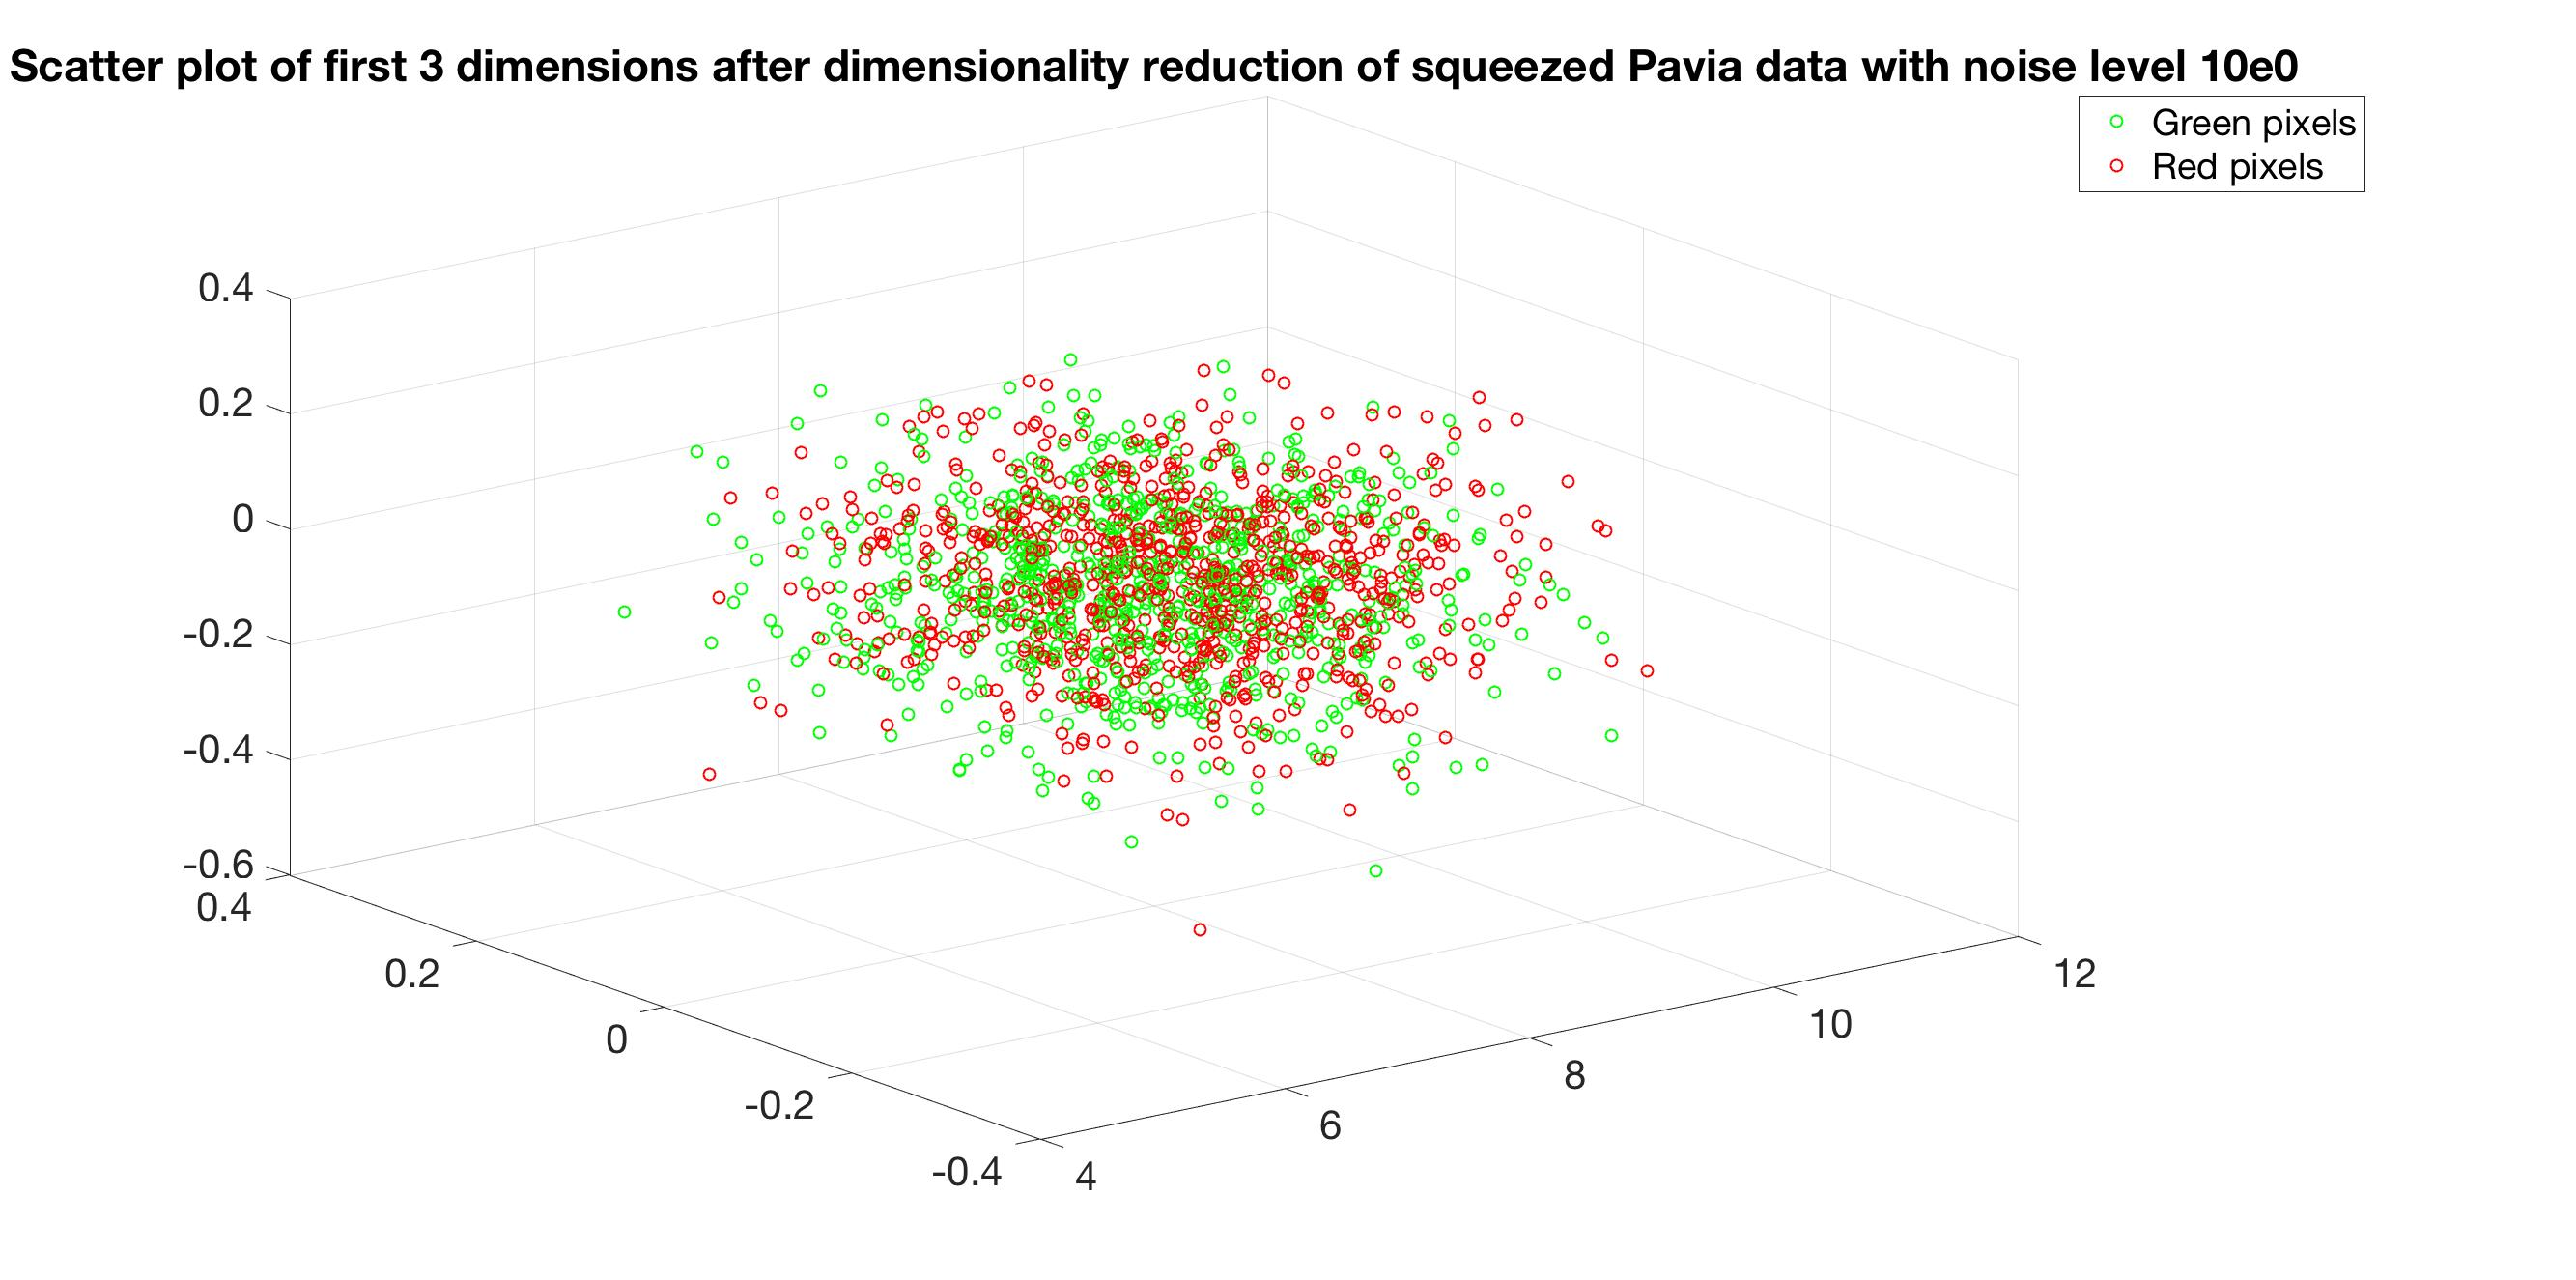
\includegraphics[width=.18\linewidth]{Noisescattermnfsqueezed0.jpg}}}	
	\subfloat{{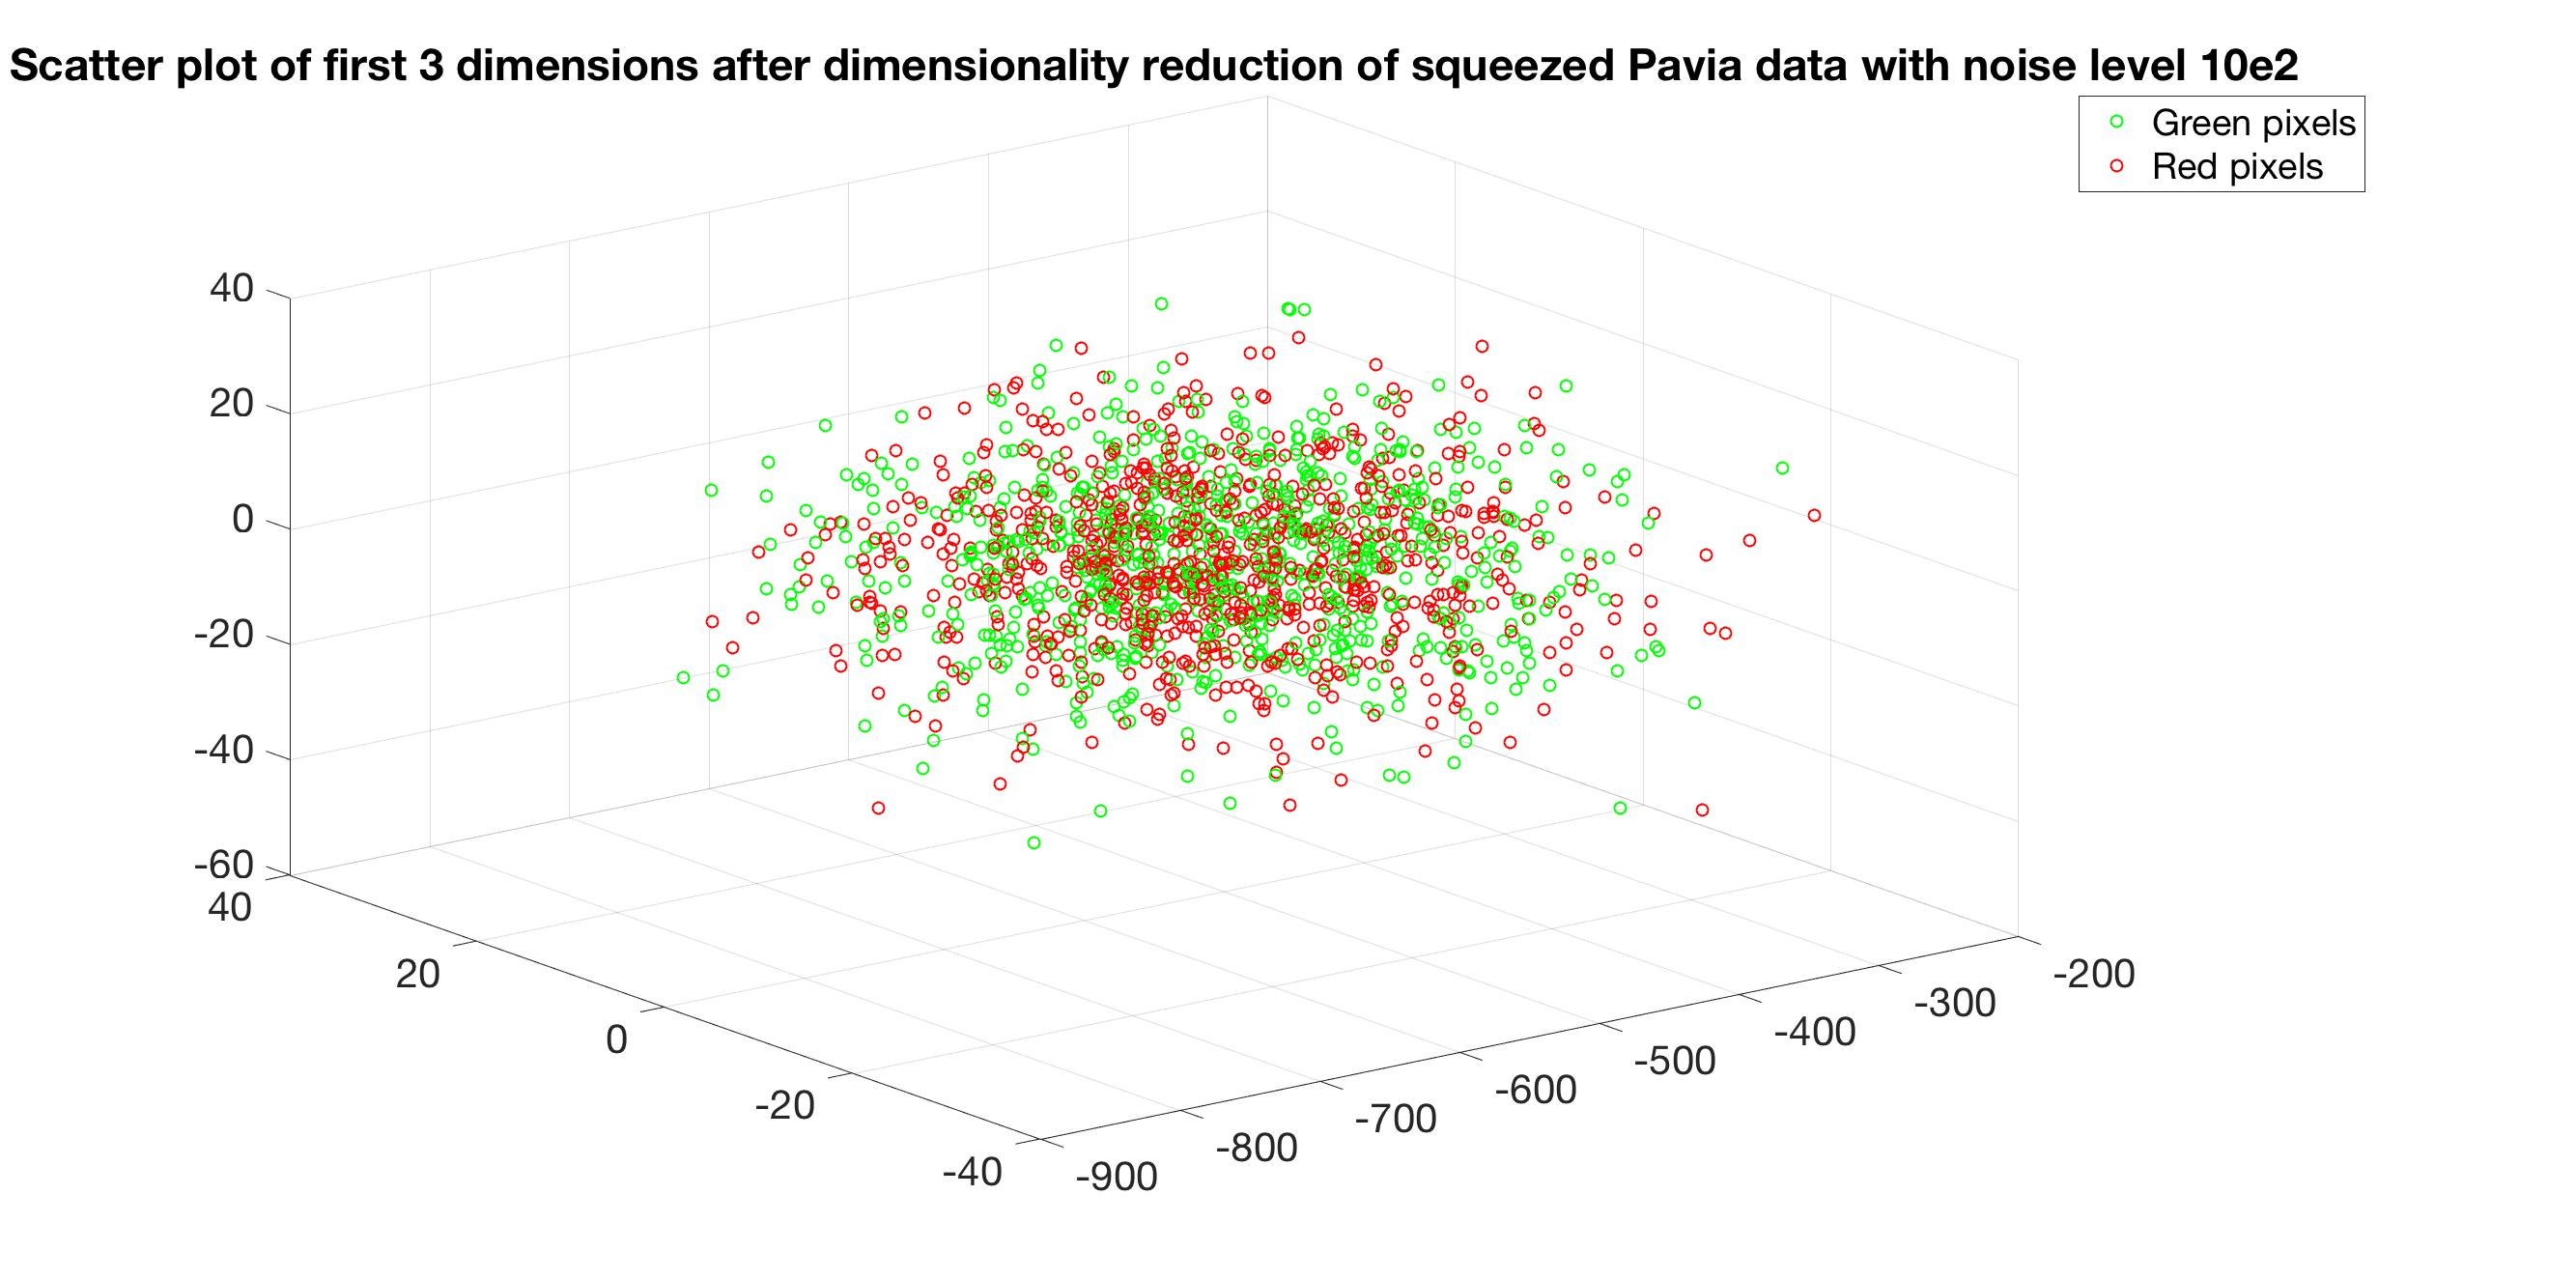
\includegraphics[width=.18\linewidth]{Noisescattermnfsqueezed2.jpg}}}	
	\subfloat{{\includegraphics[width=.18\linewidth]{Noisescattermnfsqueezed4.jpg}}}	
	\caption{Scatter plot of first 3 components after dimensionality using MNF with noise added to the squeezed fake Pavia image}
	\label{sqPaviamnfscatter}
\end{figure}

The diagonal loading factor are changed to be $10^{-4}$, $10^{-2}$, $1$, $10^{2}$, $10^{4}$. The mean over all bands with dimension reduced with fake Pavia image are shown in figure \ref{Paviamnfdiag}; the corresponding scatter plot of first 3 components after dimensionality using MNF are shown in figure  \ref{PaviamnfdiagScatter}. The mean over all bands with dimension reduced with squeezed fake Pavia image are shown in figure \ref{sqPaviamnfdiag}; the corresponding scatter plot of first 3 components after dimensionality using MNF are shown in figure  \ref{sqPaviamnfdiagScatter}.

\begin{figure}[H]
	\centering
	\subfloat{{\includegraphics[width=.18\linewidth]{mnfdiag-4.jpg}}}
	\subfloat{{\includegraphics[width=.18\linewidth]{mnfdiag-2.jpg}}}	
	\subfloat{{\includegraphics[width=.18\linewidth]{mnfdiag0.jpg}}}	
	\subfloat{{\includegraphics[width=.18\linewidth]{mnfdiag2.jpg}}}	
	\subfloat{{\includegraphics[width=.18\linewidth]{mnfdiag4.jpg}}}	
	\caption{Scatter plot of first 3 components after dimensionality with different diagonal loading factors on fake Pavia image}
	\label{Paviamnfdiag}
\end{figure}

\begin{figure}[H]
	\centering
	\subfloat{{\includegraphics[width=.18\linewidth]{scattermnf-4.jpg}}}
	\subfloat{{\includegraphics[width=.18\linewidth]{scattermnf-2.jpg}}}	
	\subfloat{{\includegraphics[width=.18\linewidth]{scattermnf0.jpg}}}	
	\subfloat{{\includegraphics[width=.18\linewidth]{scattermnf2.jpg}}}	
	\subfloat{{\includegraphics[width=.18\linewidth]{scattermnf4.jpg}}}	
	\caption{Scatter plot of first 3 components after dimensionality using MNF with different diagonal loading factors on fake Pavia image}
	\label{PaviamnfdiagScatter}
\end{figure}

\begin{figure}[H]
	\centering
	\subfloat{{\includegraphics[width=.18\linewidth]{mnfdiagsqueezed-4.jpg}}}
	\subfloat{{\includegraphics[width=.18\linewidth]{mnfdiagsqueezed-2.jpg}}}	
	\subfloat{{\includegraphics[width=.18\linewidth]{mnfdiagsqueezed0.jpg}}}	
	\subfloat{{\includegraphics[width=.18\linewidth]{mnfdiagsqueezed2.jpg}}}	
	\subfloat{{\includegraphics[width=.18\linewidth]{mnfdiagsqueezed4.jpg}}}	
	\caption{Scatter plot of first 3 components after dimensionality with different diagonal loading factors on squeezed fake Pavia image}
	\label{sqPaviamnfdiag}
\end{figure}

\begin{figure}[H]
	\centering
	\subfloat{{\includegraphics[width=.18\linewidth]{scattermnfsqueezed-4.jpg}}}
	\subfloat{{\includegraphics[width=.18\linewidth]{scattermnfsqueezed-2.jpg}}}	
	\subfloat{{\includegraphics[width=.18\linewidth]{scattermnfsqueezed0.jpg}}}	
	\subfloat{{\includegraphics[width=.18\linewidth]{scattermnfsqueezed2.jpg}}}	
	\subfloat{{\includegraphics[width=.18\linewidth]{scattermnfsqueezed4.jpg}}}	
	\caption{Scatter plot of first 3 components after dimensionality using MNF with different diagonal loading factors on squeezed fake Pavia image}
	\label{sqPaviamnfdiagScatter}
\end{figure}

\section{Discussion}
Before discussing each individual experiment it is important to note a few main factors that effect all testing results. All parameters for our testing results were selected directly from our cross-validated training results. It is also important to recall our removal of bad bands. Each dimensionality reduction method depends upon the data given to it, if there are any errors in our bad band removal step as described in section A of the methodology, these will be passed through to the rest of the experiments. Lastly, due to spectral down sampling needing to be passed a number at least or lower than half of the amount of features originally used, we did not experiment with dimensionality greater than half the original dimensionality after removing bad bands.

Within our investigation into PCA, we noticed that training on a per class basis was more successful than the entire image for higher numbers of principal components as seen in figure \ref{fig:PCAEXPCval}. In our view, this occurs because of what PCA aims to do in the first place - project the data in directions of decreasing variance. When a single transform is used (full image plot), the data is projected into directions that represent the most variance for the entire image and not on a class by class basis. It is fairly intuitive that by building a transformation that maximizes variance specifically for each class, performance should be improved. Each class should have a unique transformation that helps to separate it from others. Another interesting plot shown in figure \ref{fig:PCAEXPVar} demonstrates that although we have many many features, variance can be maximized in around 10-20 principal components. This does not mean that only 10-20 of our features are useful or contain variance. This merely states that based on a single experiment from the training data, the data can be projected into a new space where 10-20 principal components contain almost all of the variance. At around 3 principal components, $97\%$ of the variance is preserved. Does this mean that those 3 components that contain most of the variance can also separate the data? Not necessarily. As seen in figure \ref{PCAEXP3D}, although the top 3 principal components contain $>95\%$ of the variance, these 3 components do not separate the classes. We included the plot of the bottom 3 components to show that neither maximum nor minimum variance in the PCA space can separate these classes. 

For the method of Maximum Noise Fraction, a fake image is used to add noise. The performance of it, however, is worst, mainly result from the fact that MNF need spatial information, which is not exist in the fake image. When we look at the first and last three MNF components after dimensionality reduction, we can see that the magnitude of the reflectance of the first three bands are much larger than the last three, which is true that MNF is able to order components in terms of image quality. Another thing we looked at is the effects of the levels for both noise covariance as well as the diagonal loading factor. It is obvious that with increasing level of noise, the performance of classification would decrease. As it makes a lot sense since higher level of noise would make the problem harder. As for the diagonal loading factor, no obvious influence is observed regarding the final result of classification.

Before a deeper investigation into Hierarchical Clustering, we verified the computation of KL-divergence as seen in figure \ref{fig:HDRMostSim}. In figure \ref{HDREXP}, there are slight differences in classification accuracy, however it is important to remember this is for 10 experiments. Random initializations of the training data can cause slight variations in the features chosen during HDR and consequently the classification accuracy. Overall HDR performs relatively robustly with small changes in classification accuracy when removing small numbers of features. The largest change in performance happens between 10 and 20 features and this drop can be seen in other methods. As a result of this trend over all other methods we consider this to be inherent to the data chosen and the difficulty of separating the two classes.

Lastly, we investigated down sampling by simply averaging bands. This is by far the most intuitive method and it shows some interesting results when compared with the other methods on the training data in a cross-validation scheme. In both full and per class training methods, down sampling has comparable performance with HDR until around 60 features. This leads to an interesting question that can not be answered given the time allotted for this investigation: could a combined down sampling and HDR method be used to quickly reduce dimensionality of data for a classification approach? As can be easily understood, HDR relies on a square similarity matrix. Instead of computing this large matrix from the beginning, maybe some bands can be initially averaged and then a much smaller similarity matrix can be constructed to enhance the speed of computation? This is outside of the scope of our problem, but an interesting question nevertheless.

For the Pavia dataset, we look closely to the effects of noise level as well as diagonal loading level to dimensionality reduction performance using MNF. It is clearly shown that when the noise level increases, the image becomes hard to recognize. However it is interesting to find that with dimension reduced, the image becomes clear. Also, it is obvious that with increasing level of noise added, the classes become less separable. When we change the value for the diagonal loading factor, no obvious changes is observed.

\bibliography{DimRedPaper}
\bibliographystyle{ieeetr}



\end{document}
